%*******************************************************************
%   Project: DysLex-Probe Thesis (BRAC University CSE400)
%   
%   Supervisor: Dr. Farig Sadeque
%   Build with XeLaTeX (Bangla characters require fontspec, not inputenc)
%*******************************************************************

\documentclass[12pt,oneside,openany]{report}

% ====================================================================
%  DRAFT / FAST-COMPILE SWITCH  (helps avoid Overleaf compile timeouts)
%
%  \draftmodefalse  = FINAL build: full thesis, all images, bibliography
%                     and Appendix B included. USE THIS FOR SUBMISSION.
%  \draftmodetrue   = FAST build: images render as empty boxes, and the
%                     bibliography and the heavy Bangla Appendix B are
%                     skipped, so the document compiles in a fraction of
%                     the time while you edit. Citations will show as [?]
%                     and references to Appendix B stay unresolved; this
%                     is expected in draft mode. Switch back to
%                     \draftmodefalse before producing the final PDF.
% ====================================================================
\newif\ifdraftmode
\draftmodefalse   % <-- set to \draftmodetrue to fast-compile while editing

\usepackage[a4paper,width=150mm,top=25mm,bottom=25mm]{geometry}
\usepackage{fontspec}
\usepackage{csquotes}
\usepackage{amsmath}
\usepackage{amssymb}
\usepackage{bm}
\usepackage{booktabs}
\usepackage{multirow}
\usepackage{longtable}
\usepackage{xcolor}
\pagestyle{plain}

\ifdraftmode
  \usepackage[draft]{graphicx}  % draft: skip image loading -> boxes only (fast)
\else
  \usepackage{graphicx}
\fi
\graphicspath{{images/}}
\usepackage{caption}
\usepackage{subcaption}
\usepackage{array}
\usepackage{float}
\usepackage{adjustbox}     % provides max width=... for tables
\usepackage{tabularx}      % full-block tables that fill \textwidth and wrap
% Full-block column types: Y = centred wrapping, L = left wrapping, R = right wrapping
\newcolumntype{Y}{>{\centering\arraybackslash}X}
\newcolumntype{L}{>{\raggedright\arraybackslash}X}
\newcolumntype{R}{>{\raggedleft\arraybackslash}X}

\usepackage[nottoc]{tocbibind}

\PassOptionsToPackage{hyphens}{url}  % allow long URLs to break at slashes/hyphens
\usepackage{hyperref}
\hypersetup{
    colorlinks=true,
    linkcolor=black,
    filecolor=magenta,
    urlcolor=black,
    citecolor=black,
}
\urlstyle{same}

\setlength{\parindent}{0em}
\setlength{\parskip}{0.6em}

% --- Prevent text from running outside the right margin (overfull \hbox) ---
% Let TeX stretch tight lines a little instead of overflowing the margin.
\setlength{\emergencystretch}{3em}
% Long file/identifier names in \texttt{...} contain \_ which cannot break by
% default; allow an invisible break opportunity after each underscore so paths
% such as results\_mt5\_localization\_depth\_scan.csv wrap instead of overflowing.
\renewcommand{\_}{\textunderscore\allowbreak}

% Bangla font: Noto Serif Bengali has full conjunct (yuktoborno) coverage;
% FreeSerif renders conjuncts as missing glyphs (the ??? problem). XeLaTeX's
% native shaper handles Bengali ligatures with Script=Bengali. On Overleaf and TeX Live.
\newfontfamily\banglafont[Script=Bengali]{Noto Serif Bengali}

\usepackage{nomencl}
\renewcommand{\nompreamble}{The next list describes symbols and abbreviations used in the body of this thesis.}
\makenomenclature

% Plain BibTeX (faster than biblatex+biber)
\let\cleardoublepage=\clearpage

\begin{document}

\thispagestyle{empty}
\begin{titlepage}
\renewcommand*{\thepage}{Title}

    \begin{center}
        \vspace*{2cm}

        {\fontsize{18pt}{24pt}\selectfont\textbf{Probing Cross-Lingual Lexical Representations in Multilingual Large Language Models for Low-Resource Dyslexia Screening}}

        \vspace{1.5cm}

        \text{by}

        \vspace{0.5cm}

            Ayesha Siddika\\
            24341144\\
            Miss Nazmoon Nahar Aka\\
            22101649\\
            Mashrafi Rahman\\
            24341197\\
            Hasan Mohammad Sayem\\
            22101116

        \vspace{1.5cm}

            A thesis submitted to the Department of Computer Science and Engineering\\
            in partial fulfillment of the requirements for the degree of\\
            B.Sc. in Computer Science and Engineering

        \vspace{2.5cm}

            Department of Computer Science and Engineering\\
            BRAC University\\
            May 2026.

        \vspace{3cm}

            \copyright\ 2026. BRAC University\\
            All rights reserved.

    \end{center}

\end{titlepage}

\cleardoublepage

\pagenumbering{roman}

\phantomsection
\addcontentsline{toc}{chapter}{Declaration}
\newcommand*\wildcard[2][6cm]{\vspace{2cm}\parbox{#1}{\hrulefill\par#2}}

\section*{Declaration}

It is hereby declared that

\begin{enumerate}
  \item The thesis submitted is our own original work while completing the degree at BRAC University.
  \item The thesis does not contain material previously published or written by a third party, except where this is appropriately cited through full and accurate referencing.
  \item The thesis does not contain material which has been accepted, or submitted, for any other degree or diploma at a university or other institution.
  \item We have acknowledged all main sources of help.
\end{enumerate}

\vspace{1cm}
\textbf{Students' Full Name \& Signature:}

\begingroup

    \begin{center}
        \wildcard{\centerline{Ayesha Siddika} ~\\ \centerline{24341144}}
        \hspace{2cm}
        \wildcard{\centerline{Miss Nazmoon Nahar Aka} ~\\ \centerline{22101649}}

        \wildcard{\centerline{Mashrafi Rahman} ~\\ \centerline{24341197}}
        \hspace{2cm}
        \wildcard{\centerline{Hasan Mohammad Sayem} ~\\ \centerline{22101116}}
    \end{center}

\endgroup

\pagebreak


\phantomsection
\addcontentsline{toc}{chapter}{Approval}
\section*{Approval}

The thesis titled ``Probing Cross-Lingual Lexical Representations in Multilingual Large Language Models for Low-Resource Dyslexia Screening'' submitted by
\begin{enumerate}
  \item Ayesha Siddika (24341144)
  \item Miss Nazmoon Nahar Aka (22101649)
  \item Mashrafi Rahman (24341197)
  \item Hasan Mohammad Sayem (22101116)
\end{enumerate}

of Spring 2026 has been accepted as satisfactory in partial fulfillment of the requirement for the degree of B.Sc. in Computer Science and Engineering in Spring 2026.

\vspace{0.5cm}
\textbf{Examining Committee:}

\vspace{1cm}

Supervisor:\\
(Member)
\begin{center}
    \hspace{7cm} \wildcard{\centerline{Dr. Farig Yousuf Sadeque} ~\\ \centerline{Assistant Professor}~\\ \centerline{Department of Computer Science and Engineering}~\\ \centerline{BRAC University} } \hspace{1cm}
\end{center}

Co-Supervisor:\\
(Member)
\begin{center}
    \hspace{7cm} \wildcard{\centerline{Mr. Md. Tanzim Reza} ~\\ \centerline{Lecturer}~\\ \centerline{Department of Computer Science and Engineering}~\\ \centerline{BRAC University} } \hspace{1cm}
\end{center}

Program Coordinator:\\
(Member)
\begin{center}
    \hspace{7cm} \wildcard{\centerline{Name of Program Coordinator} ~\\ \centerline{Designation}~\\ \centerline{Department of Computer Science and Engineering}~\\ \centerline{BRAC University} } \hspace{1cm}
\end{center}

Head of Department:\\
(Chair)
\begin{center}
    \hspace{7cm} \wildcard{\centerline{Name of Head of Department} ~\\ \centerline{Professor and Chairperson}~\\ \centerline{Department of Computer Science and Engineering}~\\ \centerline{BRAC University} } \hspace{1cm}
\end{center}

\pagebreak


\phantomsection
\addcontentsline{toc}{chapter}{Ethics Statement}
\section*{Ethics Statement}

This study used no human participants, no clinical data and no personally identifying information. The stimulus dataset comprises 440 isolated English and Bangla words and short phrases generated and verified by the author. Bangla items were checked by a native speaker for orthographic validity. All linguistic resources are publicly available or generated for this work.

All model weights probed in this thesis (XLM-RoBERTa large, Llama 3.1 8B, BLOOM 7B1 and mT5 XL) are publicly released by their respective providers and were used in a frozen, read-only manner; no fine-tuning, no parameter updates and no redistribution of weights occurred. Use complied with each model's published license. No clinical claim is made; the work is a methodological and mechanistic study and the screening application is positioned as future, supervised clinical research.

\pagebreak


\phantomsection
\addcontentsline{toc}{chapter}{Abstract}
\section*{Abstract}

Dyslexia screening in low-resource languages is constrained by the scarcity of expert clinicians, validated test batteries and labelled corpora. Multilingual large language models (LLMs) are an attractive substrate because their pretraining already encodes substantial cross-lingual structure, but it is not known which architectures actually carry lexical and phonological information that transfers from a high-resource source (English) to a low-resource target (Bangla), nor where in the network such information lives. This thesis probes four publicly released multilingual LLMs that span the four dominant pretraining recipes -- XLM-RoBERTa large (multilingual masked encoder, 0.56B), Llama 3.1 8B (English-heavy causal decoder), BLOOM 7B1 (46-language causal decoder) and mT5 XL (multilingual span-corruption encoder-decoder, 3.7B). A curated set of 440 stimuli (220 English + 220 Bangla) spanning seven phonological task families is fed through each frozen model, and per-layer linear probes are trained for voicing, real-versus-pseudo word, orthographic transparency and syllable count.

A central methodological finding is that three of these four standard tasks fail surface-feature sanity checks: voicing labels are recoverable from the first character alone, orthographic and syllable probes do not improve over a five-feature character-statistic baseline, and the apparent cross-lingual signal in prior work largely reflects character statistics or token identity rather than phonological structure. After length-matched stimulus reconstruction, only real-versus-pseudo word discrimination survives. On this surviving task, BLOOM reaches 0.92 F1 on Bangla zero-shot transfer and XLM-R reaches 0.86 F1 with only 0.56B parameters, while Llama (0.63 F1) and mT5 (0.60 F1) collapse to surface-baseline level for cross-lingual transfer. Representational Similarity Analysis (RSA) and causal forward-hook ablation confirm that BLOOM and XLM-R distribute cross-lingual lexical information widely, whereas mT5 alone localises it: zeroing ten ranked units in the encoder selectively impairs Bangla transfer by 0.11--0.14 F1 across all probed encoder depths, and two units (782 and 1880) persist as a backbone across more than half of those depths. The thesis concludes with a paired recommendation -- BLOOM 7B1 for practical low-resource Bangla screening prototypes and mT5 XL for interpretable, mechanism-revealing analyses -- and with a methodology contribution: surface-matched stimuli plus native-verified labels are the minimum standard for any future clinical probing of multilingual LLMs.

\vspace{1cm}
\textbf{Keywords:} dyslexia screening; multilingual large language models; cross-lingual transfer; probing; representational similarity analysis; causal ablation; low-resource Bangla NLP; mechanistic interpretability.
\pagebreak


\phantomsection
\addcontentsline{toc}{chapter}{Dedication}
\section*{Dedication}

To the children whose reading difficulties remain invisible only because no test exists in their language, and to the families and teachers who notice anyway.

\pagebreak


\phantomsection
\addcontentsline{toc}{chapter}{Acknowledgment}
\section*{Acknowledgement}

We are deeply grateful to our supervisor, Dr.~Farig Yousuf Sadeque, and our co-supervisor, Mr.~Md.~Tanzim Reza, for the latitude to chase a methodological question to its uncomfortable conclusion and for steady, sharp feedback when the surface-feature sanity checks reframed the entire study halfway through. We thank the Department of Computer Science and Engineering at BRAC University for compute access, and the maintainers of the Hugging Face ecosystem, PyTorch, scikit-learn, Unsloth and the model providers behind XLM-RoBERTa, Llama, BLOOM and mT5 for making frozen-model probing technically possible without institutional resources. A native-speaker reviewer kindly verified the Bangla stimulus set; remaining errors are ours. Finally, to our families, who tolerated months of GPU-fan noise and absent dinners: thank you.

\pagebreak


\renewcommand{\contentsname}{Table of Contents}
\cleardoublepage
\phantomsection
\addcontentsline{toc}{chapter}{Table of Contents}
\tableofcontents

\listoffigures
\listoftables

\printnomenclature
\addcontentsline{toc}{chapter}{Nomenclature}
\cleardoublepage

\pagenumbering{arabic}

\chapter{Introduction}
\section{Background}

Developmental dyslexia is a specific learning difficulty that impairs accurate and fluent word reading, decoding and spelling despite adequate intelligence, schooling and sensory function \cite{snowling2020dyslexia,peterson2012developmental}. Estimated prevalence in school-age populations ranges from five to twelve percent depending on language, diagnostic threshold and writing system, with deeper, less transparent orthographies such as English producing higher functional impairment than shallow orthographies such as Spanish or Finnish \cite{ziegler2005reading,wagner2020prevalence}. The dominant cognitive account is the \emph{phonological deficit hypothesis}: dyslexic readers show weakness in representing, retrieving and manipulating speech sounds, which propagates into slower and less accurate grapheme-to-phoneme mapping during reading acquisition \cite{snowling2020dyslexia,goswami2011temporal}.

The clinical pathway depends on standardised, language-specific test batteries (e.g.\ CTOPP-2 \cite{wagner2013ctopp}, TOWRE-2, the Bangla-language tools described by Nag and colleagues \cite{nag2014dyslexia,nag2017indian}). These instruments require trained psychometricians, take 30--90 minutes to administer and are not available in most of the world's languages. Bangla, with more than 270 million speakers, has no widely deployed normative dyslexia screening tool and no consensus diagnostic battery; suspected cases are routinely identified only at the secondary-school level or not at all \cite{nag2014dyslexia,nag2017indian,badsha2024mall}. The cost of this gap is conservatively counted in millions of children whose reading failure is interpreted as low ability or low motivation.

In parallel, multilingual large language models (LLMs) have crossed a capability threshold at which their hidden representations encode rich, transferable linguistic structure across the languages in their pretraining mix \cite{conneau2020xlmr,scao2022bloom,dubey2024llama3,xue2021mt5}. The same models that drive translation, search and dialogue systems are also accumulating, as a by-product, the kind of lexical and sub-lexical structure that clinical screening tools probe explicitly. If that structure can be \emph{transferred} from a resource-rich language (English, where validated probes and labelled corpora exist) to a low-resource language (Bangla, where they do not), then a single multilingual model could in principle anchor a family of screening prototypes across many languages at once.

\section{Rationale of the Study or Motivation}

Two recent observations motivate the study. First, prior probing work on multilingual LLMs reports striking cross-lingual transfer of phonological and lexical features \cite{conneau2020xlmr,pires2019mbert,wu2020emerging}, but most of that work uses unmatched stimuli: surface confounds such as character length, byte length and orthographic baseline frequencies are not controlled. A probe that ``recovers voicing'' may, on inspection, be reading the first character of the word rather than any phonological feature. The first motivation is therefore to apply tight surface-feature sanity controls to standard phonological probing tasks and test whether the reported cross-lingual effects survive.

Second, low-resource clinical applications of LLMs are constrained by both data and compute. A useful screening prototype must (i) work zero-shot from a high-resource source language because labelled Bangla data are scarce; (ii) be interpretable, because clinical deployment cannot rely on opaque scoring; and (iii) be parameter-efficient, because Bangladesh-region deployments often run on consumer hardware. No prior study compares the four canonical pretraining recipes -- multilingual masked encoder, English causal decoder, multilingual causal decoder and multilingual span-corruption encoder-decoder -- on the same surface-controlled cross-lingual lexical task with the same stimuli, on the same hardware. This thesis closes that gap.

\section{Problem Statement}
\label{sec:rqs}

Despite repeated claims that multilingual LLMs encode transferable phonological and lexical structure, no published study (i) verifies these claims under surface-feature sanity controls, (ii) compares across the four dominant pretraining recipes with shared stimuli and shared metrics, and (iii) localises the cross-lingual lexical signal causally in the network. The practical consequence is that a clinician or NLP engineer asked to build a Bangla dyslexia screening prototype has no principled basis for choosing a model family, no estimate of expected transfer once surface confounds are removed, and no map of where the relevant computation lives. The problem this thesis addresses is therefore: \emph{which multilingual LLM family carries cross-lingual lexical information that survives surface-feature controls, how much information transfers from English to Bangla, and where in the network does it reside?}

\textbf{Research questions.} The problem above is decomposed into four research questions that structure the empirical work and map one-to-one onto the result sections of Chapter~5.

\begin{description}
    \item[RQ1 (in-language encoding).] Can a frozen multilingual LLM encode phonological and lexical features (voicing, real vs.\ pseudo word, orthographic transparency, syllable count) such that those features are linearly recoverable from per-layer hidden states on English stimuli, and at which layers do they emerge?

    \item[RQ2 (cross-lingual transfer).] Does the encoding measured in RQ1 transfer zero-shot from English to Bangla once stimulus-level surface confounds (first-character identity, character-statistic baselines and 1:1 character-length matching) are controlled?

    \item[RQ3 (mechanism and localisation).] For models that exhibit cross-lingual transfer in RQ2, is the responsible information distributed across many hidden units or causally localised to a small subset, and if localised, does the subset persist across encoder depth?

    \item[RQ4 (architecture and model selection).] Which combination of pretraining objective (masked encoder, causal decoder, span-corruption encoder-decoder) and pretraining language coverage (English-heavy vs.\ multilingual with explicit Bangla coverage) best supports surface-controlled cross-lingual lexical transfer at consumer-GPU parameter scale, and what is the resulting principled recommendation for downstream low-resource Bangla screening prototypes?
\end{description}

\section{Objective}

The general objective is to identify which publicly available multilingual LLM is the best substrate for a low-resource Bangla dyslexia-screening prototype and to expose, at the unit level, how cross-lingual lexical representations are organised. The specific objectives are:

\begin{enumerate}
    \item Curate a 440-stimulus phonological dataset (220 English + 220 Bangla) spanning seven dyslexia-relevant task categories and verify Bangla items with a native speaker (Appendix~B).
    \item Probe four publicly released multilingual LLMs -- XLM-RoBERTa large, Llama 3.1 8B, BLOOM 7B1 and mT5 XL -- using frozen per-layer linear probes on four phonological tasks: voicing, real vs.\ pseudo word, orthographic transparency and syllable count.
    \item Apply surface-feature sanity controls (first-character lookup baseline, five-feature character-statistic baseline, character-length matching) and determine which tasks reflect genuine phonological coding versus surface artefacts.
    \item Measure zero-shot cross-lingual transfer from English to Bangla on the surviving task using length-matched stimuli, and quantify per-model transfer gain above surface baselines.
    \item Use Representational Similarity Analysis (RSA) and causal forward-hook ablation to characterise whether cross-lingual lexical information is distributed or localised in each model, and to identify persistent units across encoder depth where applicable.
    \item Issue a model-selection recommendation grounded in surface-controlled performance, interpretability and parameter efficiency.
\end{enumerate}

\section{Methodology in Brief}

Four publicly released multilingual LLMs are loaded in their official pretrained form and frozen. The 440-stimulus dataset is fed through each model with a single forward pass per item; hidden states are collected at every layer (or every encoder layer for the encoder-decoder model). For each phonological task, a per-layer linear probe (logistic regression for classification, ridge regression for syllable count) is trained on English and evaluated on English (in-language) and on Bangla (zero-shot cross-lingual). Surface-feature baselines are trained on the same labels using only character statistics. After length matching, the surviving task is re-probed and used to score Representational Similarity Analysis (RSA) and a forward-hook causal ablation that zeroes the top-$K$ probe-ranked hidden units and remeasures transfer. The mT5 encoder is re-ablated at five depths with random-unit controls to test whether localisation is layer-specific or persistent. Figure~\ref{fig:methodology-pipeline} (Chapter~4) summarises the pipeline.

\section{Scopes and Challenges}

The scope is bounded to (i) four multilingual LLM families released as of 2024, (ii) two languages (English and Bangla), (iii) word-level stimuli with sentence-level items reserved for descriptive use, and (iv) frozen, read-only probing -- no fine-tuning, no continual pretraining and no clinical deployment. The four main challenges encountered were: (1) 8B-parameter causal models do not fit in a single consumer GPU with full-precision activations across 32 layers; this is mitigated with 4-bit weight quantisation via Unsloth/BitsAndBytes \cite{dettmers2022bnb} for the Llama and BLOOM passes, while keeping probes trained on the resulting hidden states. (2) Bangla orthography includes conjuncts (\textit{yuktoborno}) whose tokenisation varies across model families, biasing surface metrics; this is addressed by computing length statistics from the original Unicode string, not the tokeniser output. (3) Most Bangla phonological labels are not publicly available; we generate them from phonotactic rules and verify with a native speaker, but discover during sanity checking that the voicing label set is fully recoverable from the first character -- a finding that reframes part of the original research question. (4) Causal ablation specificity requires a random-unit control with multiple seeds; the encoder-decoder localisation analysis is therefore the most compute-intensive part of the pipeline and is run on the smaller mT5 encoder.


\chapter{Literature Review}
\section{Preliminaries}

This chapter reviews the body of work on which the thesis builds. It is organised in three parts. The \emph{Preliminaries} introduce the cognitive science of dyslexia, the linguistic notion of orthographic depth, the architecture of multilingual large language models (LLMs), and the interpretability methods (probing, representational similarity analysis and causal ablation) that the thesis applies. The \emph{Review of Existing Research} surveys the empirical literature on cross-lingual transfer, phonological probing, automated dyslexia screening and mechanistic interpretability, and closes by positioning the thesis against this literature along six dimensions to make the research gap explicit. The \emph{Summary of Key Findings} distils the three observations from prior work that motivate the experiments of Chapters~4 and~5.

\subsection{Developmental dyslexia: definition, prevalence and diagnostic criteria}

Developmental dyslexia is a specific learning difficulty of neurobiological origin, characterised by unexpected difficulty in accurate or fluent word recognition and by poor spelling and decoding, despite adequate instruction, intelligence and sensory acuity \cite{lyon2003definition,snowling2020dyslexia,peterson2012developmental}. The widely cited consensus definition of Lyon, Shaywitz and Shaywitz \cite{lyon2003definition} frames these difficulties as a consequence of a deficit in the phonological component of language, and stresses that the difficulty is \emph{unexpected} relative to other cognitive abilities. Vellutino and colleagues, in their four-decade review of specific reading disability \cite{vellutino2004specific}, reinforce this view and argue against earlier perceptual and visual accounts, locating the core impairment in language rather than in vision.

Estimates of prevalence vary with the language, the severity threshold and the cut-off convention adopted, but reading difficulty consistent with dyslexia is commonly reported in a substantial minority of school-age children \cite{vellutino2004specific,wagner2020prevalence}. Wagner and colleagues \cite{wagner2020prevalence} note that prevalence figures are highly sensitive to the operational definition used, which complicates cross-study and cross-language comparison. Diagnosis in clinical practice rests on standardised batteries that contrast reading and reading-related skills against age and grade norms; the absence of such norms for many languages, including Bangla, is itself a barrier to identification and is one of the motivations for the present work.

\subsection{The phonological deficit hypothesis and competing accounts}

The most strongly supported cognitive account of dyslexia is the \emph{phonological deficit hypothesis}: dyslexic readers under-represent or slowly access the speech-sound structure of language, which compromises the learning of grapheme-to-phoneme correspondences and slows reading acquisition \cite{snowling2020dyslexia,goswami2011temporal,wagner1987nature}. Wagner and Torgesen \cite{wagner1987nature} laid early groundwork by showing that phonological processing abilities are causally implicated in the acquisition of reading skills rather than being a mere by-product of reading experience. Share \cite{share1995phonological} extended this into the self-teaching hypothesis, in which phonological recoding is the mechanism by which children build up orthographic knowledge: each successful decoding of a novel word provides an opportunity to learn its spelling, so a phonological weakness compounds over time into an orthographic one.

The phonological account is not the only one on offer. Ramus and colleagues \cite{ramus2003theories}, in a multiple-case study of dyslexic adults, evaluate the phonological theory alongside auditory, visual-magnocellular and cerebellar theories, and conclude that a phonological deficit is present in the great majority of cases, while sensorimotor difficulties, where they occur, are neither necessary nor sufficient to explain the reading impairment. The temporal-processing account of Goswami \cite{goswami2011temporal} situates the phonological deficit within a broader difficulty in tracking the temporal structure of the speech signal, linking low-level auditory rhythm perception to the development of phonological representations. For the purposes of this thesis the relevant point is that, across these competing accounts, phonological representation is the common locus of impairment, which is why a study that asks whether language models encode phonological structure is well aligned with the dominant theory of the disorder.

\subsection{Subdomains of phonological processing and their clinical assessment}

Phonological processing is conventionally decomposed into three subdomains \cite{wagner2013ctopp,kirby2010ran,wagner1987nature}. \emph{Phonological awareness} is the ability to detect and manipulate sound units such as phonemes, syllables and rhymes. \emph{Phonological short-term memory} is the ability to hold sound sequences in working memory, as probed by non-word repetition and digit-span tasks. \emph{Rapid automatised naming} (RAN) is the speed of retrieving phonological codes for visually presented stimuli such as letters, digits, colours or objects; Kirby and colleagues \cite{kirby2010ran} review the predictive relationship between naming speed and later reading and discuss its instructional implications.

These subdomains are operationalised in standardised clinical batteries. The Comprehensive Test of Phonological Processing (CTOPP-2) is the dominant instrument for English \cite{wagner2013ctopp}, probing awareness, memory and naming with subtests built from real words, pseudo-words, sound blending and elision. For South-Asian languages, Nag and colleagues \cite{nag2014dyslexia,nag2017indian} have argued that assessment cannot simply be transplanted from alphabetic English because the akshara-based writing systems of the region place different demands on the learner, and they propose assessment approaches sensitive to syllabic and akshara structure. The stimulus design used in this thesis (Chapter~4) draws its task formats from this clinical tradition: minimal-pair discrimination, real-word and pseudo-word contrasts, and syllable-level manipulations, recast as inputs whose representations can be probed in a language model.

\subsection{Computational models of word recognition}

A parallel tradition models the reading process computationally, and these models clarify what it means for a system to encode phonological versus orthographic structure. The distributed, developmental model of Seidenberg and McClelland \cite{seidenberg1989distributed} treats word recognition as the settling of a connectionist network that maps orthography to phonology through distributed hidden representations, without explicit rules or a lexicon. The dual-route cascaded (DRC) model of Coltheart and colleagues \cite{coltheart2001drc} instead posits two routes, a lexical route for known words and a non-lexical grapheme-to-phoneme route for novel strings, and accounts for the differing behaviour of regular words, irregular words and pseudo-words. These models matter for the present thesis in two ways. First, they make precise the distinction between a representation that captures the surface form of a string and one that captures its phonological realisation, which is exactly the distinction the surface-control experiments of Chapter~5 are designed to separate. Second, they motivate the use of pseudo-words as stimuli: a system that genuinely recodes orthography to phonology, rather than memorising lexical entries, should generalise to well-formed pseudo-words, and probing for phonological structure on such items tests for a recoding-like capacity in the model.

\subsection{Orthographic depth and cross-linguistic variation}

The functional impact of a phonological deficit depends on \emph{orthographic depth}: the degree of one-to-one mapping between graphemes and phonemes \cite{ziegler2005reading,katz1992reading}. The orthographic depth hypothesis of Katz and Frost \cite{katz1992reading} states that readers of shallow (transparent) orthographies can rely more heavily on a sub-lexical grapheme-to-phoneme route, whereas readers of deep (opaque) orthographies must lean more on lexical and morphological information because the surface form under-determines the pronunciation. English is opaque: one grapheme can map to many phonemes and vice versa. Shallow orthographies such as Finnish, Italian and Spanish are close to one-to-one. Bangla is intermediate: most consonants and vowels map transparently, but the script makes extensive use of conjunct characters (\textit{yuktoborno}) whose surface form does not transparently decompose into their phonological constituents, and uses the \textit{matra} headline and a range of vowel diacritics that complicate the surface-to-sound mapping.

The cross-linguistic literature reports that, at a fixed severity threshold, the apparent prevalence of dyslexia is lower in shallow orthographies, because transparent mappings make decoding easier to acquire, yet the underlying phonological deficit is comparable across orthographies \cite{ziegler2005reading,wagner2020prevalence}. Ziegler and Goswami \cite{ziegler2005reading} frame this within a psycholinguistic grain-size theory, in which readers of different orthographies converge on different optimal units of analysis (phoneme, rime, syllable, whole word) as a function of the consistency and granularity of their writing system. This body of work directly motivates the cross-lingual design of the thesis: any model representation that genuinely encodes phonological structure should generalise across orthographies of differing depth, while one that merely captures language-specific surface statistics should not, and a contrast between an opaque language (English) and an intermediate one (Bangla) is a natural setting in which to test this.

\subsection{Bangla orthography and reading acquisition}

Bangla (Bengali) is written in an abugida (alphasyllabary) in which the consonant carries an inherent vowel that is overridden by explicit vowel signs. Reading acquisition in such systems is shaped by the akshara as the functional orthographic unit, and by the visual and phonological complexity of conjunct consonants, as emphasised in the South-Asian reading-development literature \cite{nag2014dyslexia,nag2017indian}. For Bangla specifically, the most directly relevant grounding for this thesis is the dissertation of Badsha \cite{badsha2024mall}, which documents the phonological difficulty patterns of dyslexic Bangla-speaking primary-school children, including confusions of voiced and unvoiced stop pairs, errors on multisyllabic words and confusions involving the \textit{matra}. These clinician-observed patterns are adopted directly as the foundation of the stimulus design in Chapter~4: the voicing minimal pairs, the multisyllabic real-word and pseudo-word contrasts, and the \textit{matra}-sensitive items all trace back to documented Bangla difficulty categories rather than to a generic English template. Because no validated, normed automated screener exists for Bangla, and because the test infrastructure available for English has no Bangla counterpart, the language is a representative low-resource setting in which to ask whether multilingual models carry transferable phonological structure.

\subsection{The Transformer architecture and its core operations}
\label{sec:transformer-core}

Modern language models are built on the Transformer architecture of Vaswani and colleagues \cite{vaswani2017attention}, which replaced recurrence with self-attention and made it possible to train very large models on very large corpora in parallel. Because all four models studied in this thesis share this substrate, it is worth stating its core operations precisely; the architectural differences between the models, described below, are best understood as variations on these same building blocks.

A Transformer represents a sequence of tokens as a matrix of vectors and refines it through a stack of identical layers. The central operation is \emph{scaled dot-product attention}, in which each position forms a query that is compared against the keys of all positions to produce a weighted sum of their values,
\begin{equation}
\label{eq:attention}
\mathrm{Attention}(Q,K,V) = \mathrm{softmax}\!\left(\frac{QK^{\top}}{\sqrt{d_k}}\right)V,
\end{equation}
where $Q$, $K$ and $V$ are the query, key and value matrices obtained by linear projection of the layer input and $d_k$ is the key dimension; the factor $1/\sqrt{d_k}$ keeps the dot products from growing too large as dimension increases. Rather than attending once, the model attends in $h$ parallel subspaces (heads) and concatenates the results,
\begin{equation}
\label{eq:multihead}
\begin{aligned}
\mathrm{MultiHead}(Q,K,V) &= \mathrm{Concat}(\mathrm{head}_1,\dots,\mathrm{head}_h)\,W^{O}, \\
\mathrm{head}_i &= \mathrm{Attention}\!\left(QW_i^{Q},\, KW_i^{K},\, VW_i^{V}\right),
\end{aligned}
\end{equation}
with learned projections $W_i^{Q}, W_i^{K}, W_i^{V}$ and output projection $W^{O}$. Each layer follows attention with a position-wise feed-forward network applied identically at every position,
\begin{equation}
\label{eq:ffn}
\mathrm{FFN}(x) = \max(0,\, xW_1 + b_1)\,W_2 + b_2 ,
\end{equation}
and wraps each sub-layer in a residual connection followed by layer normalisation \cite{ba2016layernorm},
\begin{equation}
\label{eq:resnorm}
\mathrm{output} = \mathrm{LayerNorm}\!\left(x + \mathrm{Sublayer}(x)\right).
\end{equation}
Because attention is order-invariant, positional information must be injected separately, originally through fixed sinusoidal position encodings added to the token embeddings \cite{vaswani2017attention}. The variations that distinguish the four models, which are described per model below, lie largely in three places: how position is encoded (sinusoidal, rotary, relative bias or linear bias), which normalisation and activation the feed-forward block uses, and whether the layer stack is configured as an encoder, a decoder, or both.

\subsection{Pretraining objectives}
\label{sec:pretraining-objectives}

From this common substrate, three pretraining objectives have emerged, and they correspond to the three architectural configurations used in this thesis. \emph{Masked language modelling} (MLM), introduced at scale by BERT \cite{devlin2019bert}, corrupts a random subset $M$ of input positions and trains a bidirectional encoder to recover them from both left and right context,
\begin{equation}
\label{eq:mlm}
\mathcal{L}_{\mathrm{MLM}}(\theta) = -\,\mathbb{E}_{x}\sum_{i\in M}\log P_\theta\!\left(x_i \mid x_{\setminus M}\right),
\end{equation}
where $x_{\setminus M}$ is the sequence with the masked positions hidden. This objective yields representations optimised for understanding rather than generation. \emph{Autoregressive (causal) language modelling} (CLM), exemplified by the GPT line \cite{radford2019gpt2}, factorises the joint probability of a sequence left to right and trains a decoder to predict each token from its predecessors,
\begin{equation}
\label{eq:clm}
\begin{aligned}
P_\theta(x) &= \prod_{t=1}^{T} P_\theta\!\left(x_t \mid x_{<t}\right), \\
\mathcal{L}_{\mathrm{CLM}}(\theta) &= -\sum_{t=1}^{T}\log P_\theta\!\left(x_t \mid x_{<t}\right).
\end{aligned}
\end{equation}
\emph{Span-corruption sequence-to-sequence} pretraining, introduced by T5 \cite{raffel2020t5}, casts every task as text-to-text: contiguous spans of the input are replaced by sentinel tokens and an encoder-decoder is trained to reconstruct the dropped spans, so that for a corrupted input $\tilde{x}$ and target $y$ (the concatenation of the removed spans),
\begin{equation}
\label{eq:span}
\mathcal{L}_{\mathrm{span}}(\theta) = -\sum_{t=1}^{|y|}\log P_\theta\!\left(y_t \mid y_{<t},\, \tilde{x}\right).
\end{equation}
A further consideration specific to multilingual pretraining is corpus balancing. Because raw web corpora are dominated by high-resource languages, multilingual models up-sample low-resource languages by exponentiating the empirical language distribution with a smoothing exponent $\alpha\in(0,1)$,
\begin{equation}
\label{eq:smoothing}
q_i = \frac{p_i^{\alpha}}{\sum_j p_j^{\alpha}},
\qquad
p_i = \frac{n_i}{\sum_j n_j},
\end{equation}
where $n_i$ is the token count of language $i$; smaller $\alpha$ flattens the distribution and gives low-resource languages such as Bangla more weight. Both XLM-RoBERTa and mT5 adopt this kind of smoothing during pretraining \cite{conneau2020xlmr,xue2021mt5}.

\subsection{The four models studied}
\label{sec:four-models}

The thesis compares four publicly available multilingual models, chosen so that each instantiates a different combination of architecture and objective; contrasting them on shared stimuli isolates the effect of the pretraining recipe from that of any single model, and this cross-architecture comparison is the structural backbone of Chapter~5. Tokenisation in all four rests on subword segmentation, either byte-pair encoding \cite{sennrich2016bpe} or the SentencePiece unigram model \cite{kudo2018sentencepiece}, which matters here because it determines how a Bangla word is split before it ever reaches the network. The purpose of this section is to introduce each model at the level of its architecture and pretraining objective; the exact configuration of each checkpoint used in the experiments, including its parameter count, layer count, hidden size, tokeniser and pretraining corpus, is tabulated with the experimental setup in Chapter~4 and is not repeated here.

\subsubsection{XLM-RoBERTa (multilingual masked encoder)}

XLM-RoBERTa \cite{conneau2020xlmr} is an encoder-only Transformer trained with the masked language modelling objective of Equation~\eqref{eq:mlm} on a large multilingual corpus that includes Bangla. It follows the RoBERTa recipe, dropping BERT's next-sentence-prediction task and relying on MLM alone with a shared SentencePiece vocabulary, and it uses learned absolute position embeddings together with the GELU activation \cite{hendrycks2016gelu} in its feed-forward blocks. Because the objective is bidirectional, the hidden state at each position integrates both left and right context, which makes its representations a natural fit for the token-level probing carried out in this thesis. Its low-resource balance is governed by the corpus smoothing of Equation~\eqref{eq:smoothing}, which up-samples lower-resource languages such as Bangla.

\subsubsection{Llama 3.1 8B (English-heavy causal decoder)}

Llama 3.1 8B \cite{dubey2024llama3} is a decoder-only Transformer trained with the causal objective of Equation~\eqref{eq:clm} on a corpus that is predominantly English with comparatively little explicit multilingual coverage, which makes it the natural test of whether competence transfers to Bangla without deliberate multilingual training. It departs from the original Transformer in three architectural choices that are now standard in the Llama family. First, it normalises with RMSNorm \cite{zhang2019rmsnorm}, which rescales by the root-mean-square of the activations without subtracting the mean,
\begin{equation}
\label{eq:rmsnorm}
\mathrm{RMSNorm}(x) = \frac{x}{\sqrt{\frac{1}{d}\sum_{i=1}^{d} x_i^{2} + \epsilon}}\,\odot\, g,
\end{equation}
with a learned gain vector $g$. Second, its feed-forward block uses the SwiGLU gated activation \cite{shazeer2020glu},
\begin{equation}
\label{eq:swiglu}
\begin{aligned}
\mathrm{FFN}_{\mathrm{SwiGLU}}(x) &= \big(\mathrm{SiLU}(xW_1)\,\odot\,xW_3\big)\,W_2, \\
\mathrm{SiLU}(z) &= z\,\sigma(z),
\end{aligned}
\end{equation}
where $\sigma$ is the logistic sigmoid and $\odot$ is the elementwise product. Third, it encodes position with rotary position embeddings (RoPE) \cite{su2021roformer}, which rotate the query and key vectors by a position-dependent angle so that their inner product depends only on the relative offset,
\begin{equation}
\label{eq:rope}
\langle R_m\,q,\; R_n\,k\rangle = \langle q,\; R_{n-m}\,k\rangle,
\end{equation}
with $R_m$ a block-diagonal rotation matrix for position $m$. Its attention additionally adopts grouped-query attention, in which several query heads share a single key/value projection so as to reduce the memory cost of inference, and its subword vocabulary is built with byte-level BPE so that any Bangla string is representable even though the model is English-heavy.

\subsubsection{BLOOM 7B1 (multilingual causal decoder)}

BLOOM 7B1 \cite{scao2022bloom} is also a decoder-only model trained with the causal objective of Equation~\eqref{eq:clm}, but unlike Llama it is deliberately multilingual, pretrained on a corpus with explicit Bangla coverage; it is therefore the multilingual counterpart to Llama in the comparison. Its two distinctive architectural features are an additional layer normalisation applied immediately after the token embeddings, which stabilises training, and the use of attention with linear biases (ALiBi) \cite{press2022alibi} in place of explicit position embeddings. ALiBi adds a static, head-specific penalty to the attention logits that grows linearly with the distance between positions,
\begin{equation}
\label{eq:alibi}
\begin{aligned}
\mathrm{Attention}_{\mathrm{ALiBi}} &= \mathrm{softmax}\!\left(\frac{QK^{\top}}{\sqrt{d_k}} + m\cdot B\right)V, \\
B_{ij} &= -(i-j)\ \ \text{for}\ \ j\le i,
\end{aligned}
\end{equation}
where $m$ is a fixed slope assigned per head. Its feed-forward blocks use the GELU activation \cite{hendrycks2016gelu}.

\subsubsection{mT5 XL (multilingual span-corruption encoder-decoder)}

mT5 \cite{xue2021mt5} is the multilingual version of T5 and the only encoder-decoder among the four. It is trained with the span-corruption objective of Equation~\eqref{eq:span} on a large multilingual web corpus with explicit Bangla coverage, using the same low-resource smoothing of Equation~\eqref{eq:smoothing}. Architecturally it follows the T5.1.1 recipe: it normalises with RMSNorm \cite{zhang2019rmsnorm}, its feed-forward blocks use the GeGLU gated activation \cite{shazeer2020glu},
\begin{equation}
\label{eq:geglu}
\mathrm{FFN}_{\mathrm{GeGLU}}(x) = \big(\mathrm{GELU}(xW_1)\,\odot\,xW_3\big)\,W_2,
\end{equation}
and rather than adding positional vectors it injects \emph{relative position bias}, a learned scalar added to the attention logits as a function of the relative distance between key and query, with the bias parameters shared across all layers. Because it has a dedicated bidirectional encoder distinct from its decoder, the representations probed in this thesis are taken from the encoder stack, where, as Chapter~5 reports, the cross-lingual lexical signal turns out to be unusually concentrated.

These four models exhaust the dominant pretraining recipes in use at the time of writing -- a multilingual masked encoder, an English-heavy causal decoder, a multilingual causal decoder and a multilingual encoder-decoder -- and their controlled comparison is what allows the thesis to attribute differences in phonological encoding to the pretraining recipe rather than to incidental properties of one model.

\subsection{Subword tokenisation and its consequences for Bangla}
\label{sec:tokenisation}

None of the four models reads characters or whole words directly; each first segments text into subword units, and because this segmentation decides what the network ever ``sees'' of a Bangla word, it is worth describing the two segmentation schemes the models use and their specific consequences for an akshara-based script. The older scheme, byte-pair encoding (BPE) \cite{sennrich2016bpe}, begins with a base vocabulary of characters (or, in the byte-level variant used by Llama and BLOOM, of the 256 possible bytes) and greedily merges the most frequent adjacent pair of symbols, repeating until a target vocabulary size is reached. Writing $\mathrm{count}(a,b)$ for the corpus frequency of the adjacent pair $(a,b)$, each BPE step adds the merge
\begin{equation}
\label{eq:bpe}
(a,b)^{\ast} = \arg\max_{(a,b)}\ \mathrm{count}(a,b),
\end{equation}
so the resulting vocabulary is purely frequency-driven and contains no notion of linguistic unit. The newer scheme, the SentencePiece unigram language model \cite{kudo2018sentencepiece} used by XLM-RoBERTa and mT5, instead treats segmentation as probabilistic: it maintains a vocabulary of candidate pieces, each with a probability $p(s)$, models a tokenised sentence $\mathbf{x}=(s_1,\dots,s_M)$ as a product of piece probabilities, and selects the segmentation of highest likelihood,
\begin{equation}
\label{eq:unigram}
\begin{aligned}
P(\mathbf{x}) &= \prod_{i=1}^{M} p(s_i), \\
\mathbf{s}^{\ast} &= \arg\max_{\mathbf{s}\in \mathcal{S}(\mathbf{x})} \prod_{i=1}^{M} p(s_i),
\end{aligned}
\end{equation}
where $\mathcal{S}(\mathbf{x})$ is the set of all segmentations of the string. Neither scheme is aware of phonology or of the akshara as a unit. For Bangla this has two concrete effects that matter for the experiments. First, a conjunct character (\textit{yuktoborno}) or a vowel-diacritic-bearing akshara is frequently split across several pieces, or, under byte-level BPE, across several sub-character byte fragments, so the orthographic unit a linguist would recognise has no single corresponding vector. Second, because the first piece of a word may be a byte fragment rather than a meaningful sub-unit, a probe that keyed on the ``first token'' could be exploiting an artefact of segmentation rather than a phonological property. These two effects are exactly why the thesis pools representations across the subword pieces of each stimulus and why it includes the first-character control of Section~\ref{sec:sanity}: the tokeniser, not the model, would otherwise be a hidden confound.

\subsection{Probing as a method}

Probing trains a small supervised classifier (a ``probe'') on the frozen hidden states of a pretrained model to test whether a target linguistic property is linearly recoverable from those states \cite{conneau2018probing,hewitt2019structural}. Conneau and colleagues \cite{conneau2018probing} introduced a suite of probing tasks for sentence representations spanning surface, syntactic and semantic properties, and Hewitt and Manning \cite{hewitt2019structural} showed that syntactic tree structure is linearly recoverable from contextual word representations via a learned distance metric. The probing programme has since been used to map where and to what degree different properties are encoded; Tenney and colleagues \cite{tenney2019bert} found that the layers of BERT recapitulate the classical NLP pipeline, with lower layers carrying more local, surface and syntactic information and higher layers carrying more semantic information.

A probe that achieves above-chance accuracy is taken as evidence that the model encodes the property, while a probe at chance is taken as evidence that the property is not linearly accessible at that layer. Probing requires no model fine-tuning and isolates representational content from task-specific generation behaviour, which is why it is the central method of this thesis: the four models differ in size, objective and tokenisation, and a frozen-representation probe is the only method that compares them on a common footing without the confound of differential fine-tuning.

\subsection{Surface confounds, control tasks and information-theoretic probing}

The probing method has well-known caveats, and the literature that articulates them shapes the experimental design of this thesis. A sufficiently expressive probe can extract patterns that the model does not in fact ``use,'' so high probe accuracy does not by itself establish that a property is salient to the model \cite{belinkov2022probing}. Hewitt and Liang \cite{hewitt2019control} formalise this with \emph{control tasks}: a probe should be evaluated not only on the target task but also on a random-label control with the same input distribution, and the gap between the two (selectivity) indicates how much of the probe's success reflects the representation rather than the probe's own capacity. Pimentel and colleagues \cite{pimentel2020information} reframe probing in information-theoretic terms, arguing that probing estimates mutual information between representations and labels, and Voita and Titov \cite{voita2020mdl} propose minimum-description-length probing, which measures not just the accuracy a probe can reach but the effort (description length) needed to reach it, giving a more robust signal of how readily a property is encoded.

A distinct concern is that a probe that appears to recover a phonological target may in fact be reading a confounded surface feature, such as the first character of the string or simple character-frequency statistics, rather than the phonological property of interest \cite{belinkov2022probing,pimentel2020information}. This is the specific risk that the sanity-check experiments of this thesis are designed to address: in Section~\ref{sec:sanity} the phonological probe is compared against first-character lookup and character-statistic baselines, so that any reported phonological signal is the increment over what a trivial surface feature would already provide. To our knowledge this first-character control has not been applied in prior phonological probing of LLMs, which makes it a methodological contribution as well as a safeguard.

\subsection{Quantifying probe performance: accuracy, chance and selectivity}
\label{sec:probe-metrics}

The interpretive cautions above translate into concrete quantities that a probing study must report, and it is useful to fix the ones used throughout this thesis. The primary measure is classification accuracy, the fraction of held-out stimuli the probe labels correctly,
\begin{equation}
\label{eq:accuracy}
\mathrm{Acc} = \frac{1}{N}\sum_{i=1}^{N} \mathbf{1}\!\left[\hat{y}_i = y_i\right],
\end{equation}
where $\hat{y}_i$ is the predicted label, $y_i$ the true label and $\mathbf{1}[\cdot]$ the indicator function. Accuracy is meaningful only against a baseline: for a balanced binary distinction such as the voiced/unvoiced contrast the chance level is $0.5$, and for a $C$-way balanced task it is $1/C$, so the thesis always reports accuracy relative to chance rather than in absolute terms. To separate genuine representational content from the probe's own capacity, Hewitt and Liang \cite{hewitt2019control} define \emph{selectivity} as the gap between accuracy on the real task and accuracy on a control task that assigns the same inputs random labels,
\begin{equation}
\label{eq:selectivity}
\mathrm{Selectivity} = \mathrm{Acc}_{\mathrm{task}} - \mathrm{Acc}_{\mathrm{control}},
\end{equation}
so that a probe which scores highly only because it is expressive enough to memorise arbitrary labels is exposed by a low selectivity. The surface-control logic of this thesis is the same comparison applied to a different baseline: the reported phonological signal is the increment of the probe over a surface predictor,
\begin{equation}
\label{eq:increment}
\Delta = \mathrm{Acc}_{\mathrm{probe}} - \mathrm{Acc}_{\mathrm{surface}},
\end{equation}
where $\mathrm{Acc}_{\mathrm{surface}}$ is the accuracy of a first-character or character-statistic lookup on the same stimuli. A positive $\Delta$ is the quantity that licenses a claim about phonological encoding. Finally, the minimum-description-length view of Voita and Titov \cite{voita2020mdl} reframes the question from ``what accuracy is reachable'' to ``how compactly can the labels be described given the representation,'' reporting a code length in which a shorter description indicates a property that is more readily and robustly encoded; the thesis treats this as complementary evidence to the accuracy-based measures above.

\subsection{Representational similarity analysis and causal ablation}

Two further methods complement probing. \textbf{Representational similarity analysis (RSA)} \cite{kriegeskorte2008rsa}, imported from systems neuroscience, computes the pairwise distance matrix of model hidden states across stimuli (a representational dissimilarity matrix, or RDM) and correlates it with a reference RDM, here the RDM of the same stimuli in another language. A high cross-lingual Spearman correlation at a given layer indicates that the geometry of stimulus representations is preserved across languages, independent of any downstream probe, and so provides probe-free corroboration of cross-lingual structure. \textbf{Causal forward-hook ablation} \cite{geiger2021causal,vig2020investigating} intervenes on the forward pass by setting a chosen subset of hidden units to zero and measuring the resulting drop in probe accuracy. Vig and colleagues \cite{vig2020investigating} use such causal mediation analysis to localise where a behaviour is carried, and Geiger and colleagues \cite{geiger2021causal} develop the more general framework of causal abstraction for identifying the variables a network actually computes with. If zeroing a small ``top-$K$'' set of probe-ranked units reduces accuracy more than zeroing a random set of the same size, the information is interpreted as causally concentrated in those units; if not, it is interpreted as distributed. The thesis uses RSA in Section~\ref{sec:rq3} and causal ablation in the localisation analysis to move from correlational evidence (a probe can read the property) towards mechanistic evidence (specific units carry it).

\section{Review of Existing Research}

\subsection{Cross-lingual transfer in multilingual LLMs}

A large body of work establishes that multilingual models transfer non-trivially across languages without any explicit cross-lingual supervision. Pires and colleagues \cite{pires2019mbert} first showed that multilingual BERT achieves strong zero-shot cross-lingual transfer on part-of-speech tagging and named-entity recognition, including between languages that do not share a script, suggesting that the model learns representations that are at least partly language-neutral. Wu and Dredze \cite{wu2020emerging} surveyed mBERT across 39 languages and found that the quality of transfer is uneven and correlates with factors such as pretraining corpus size and subword overlap. Conneau and colleagues \cite{conneau2020xlmr} scaled this recipe up with XLM-RoBERTa, demonstrating that a larger model trained on more balanced multilingual data substantially improves cross-lingual natural-language inference, named-entity recognition and question answering, and that there is a transfer-interference trade-off as more languages are packed into a fixed capacity. These studies establish that multilingual masked encoders carry transferable information, but they operate at the sentence or token-label level and do not control for surface confounds at the lexical level, which is the level at which the present thesis works.

A consistent secondary finding of this literature is that the ease of transfer depends on how close the source and target languages are, whether measured by shared script, shared subword vocabulary, or typological similarity \cite{pires2019mbert,wu2020emerging}. Transfer between languages that share a script and have overlapping vocabularies is comparatively easy, whereas transfer across scripts is harder and varies widely by language pair. The English-Bangla pair studied in this thesis falls firmly on the difficult side of this divide: the two languages use entirely different scripts, share little surface vocabulary, and are typologically distant, so any cross-lingual signal recovered here cannot be attributed to the script or vocabulary overlap that makes many published transfer results easy. This makes the pair a demanding test case rather than a favourable one, and it strengthens the interpretation of a positive result while making a negative result unsurprising for the more English-centric models.

\subsection{What drives cross-lingual transfer?}

A second strand asks \emph{why} transfer happens, and its answers inform the interpretation of the thesis results. K and colleagues \cite{k2020crosslingual} dissected the cross-lingual ability of mBERT and found, perhaps counter-intuitively, that lexical (subword) overlap between languages is not the primary driver of transfer; rather, the depth of the network and the sharing of structural parameters matter more, which implies that the model learns abstractions that are not tied to shared surface forms. Artetxe and colleagues \cite{artetxe2020crosslingual} reinforced this by showing that monolingual representations can be transferred to new languages by learning only new embeddings while freezing the body of the network, demonstrating that much of what transfers lives in language-agnostic parameters rather than in a shared vocabulary. Taken together, these results suggest that a multilingual model can in principle carry abstract, surface-independent structure across languages, which is precisely the kind of structure a phonological probe with surface controls is designed to detect. They also provide a theoretical reason to expect that, if any of the four model families encodes transferable phonological structure, it need not depend on shared Bangla-English surface forms.

\subsection{Layer-wise organisation of linguistic information}

A recurring finding across the probing literature is that linguistic information is not distributed uniformly through a network but is organised by depth, which bears directly on a study that probes every layer rather than a single one. Tenney and colleagues \cite{tenney2019bert} showed that the layers of BERT recapitulate a classical natural-language-processing order, with local and surface information concentrated in lower layers, syntactic information in the middle, and more abstract, semantic information emerging higher up; they further observed that the model tends to resolve these levels in an interpretable sequence rather than all at once. Hewitt and Manning \cite{hewitt2019structural} demonstrated that this organisation is geometric as well as informational, in that syntactic tree distance is approximately recoverable as a distance in a learned subspace of the hidden states, so that the location of a property and the shape it takes jointly characterise how it is encoded. A related theme in the multilingual setting is that intermediate layers often carry the most transferable, comparatively language-neutral information, while the uppermost layers re-specialise towards the pretraining objective \cite{k2020crosslingual}. These observations motivate the layer-by-layer scan adopted in this thesis: because phonological structure could in principle surface at any depth, and because the depth at which it peaks is itself informative about how a model treats sub-lexical form, reporting a single layer would risk both missing the signal and mischaracterising it. The mT5 localisation analysis of Chapter~5, which scans depth before isolating individual units, is a direct application of this principle and is the reason the analysis reports a depth profile rather than a single headline number.

\subsection{Phonological and sub-lexical probing of LLMs}

A separate line of work probes specifically for phonological and sub-lexical content. Kann and colleagues \cite{kann2018phonological} and Chrupa\l{}a \cite{chrupala2019phonological} report that recurrent and Transformer encoders carry sub-lexical phonological structure to varying degrees, depending on the task and the layer. Hofmann and colleagues \cite{hofmann2021superbizarre} show that subword tokenisation interacts with morphology in ways that cause LLMs to encode morphological boundaries inconsistently, which is relevant because the same tokenisation pressures that distort morphology can distort the recoverability of phonological units. Soulos and colleagues \cite{soulos2021structural} probe for compositional structure in vector representations using role-learning networks, asking whether the geometry of a representation reflects a decomposable structure rather than an unanalysed whole. None of these studies tests cross-lingual transfer of phonological structure to a low-resource South-Asian language, and none applies a first-character or character-statistic control of the kind reported in Chapter~5; the present thesis is, to our knowledge, the first to bring phonological probing, cross-lingual transfer and surface controls together for Bangla.

\subsection{Critiques of probing and the move to controls}

The maturation of the probing literature has been accompanied by an internal critique that this thesis takes seriously. Belinkov \cite{belinkov2022probing}, in a survey of probing classifiers, catalogues the method's pitfalls and recommends controls and selectivity measures as standard practice. The control-task proposal of Hewitt and Liang \cite{hewitt2019control}, the information-theoretic reframing of Pimentel and colleagues \cite{pimentel2020information}, and the minimum-description-length method of Voita and Titov \cite{voita2020mdl} together represent a shift from ``can a probe recover the property'' towards ``how much of that recovery is attributable to the representation rather than the probe, and how confidently.'' The design of this thesis is squarely within this corrective tradition: it pairs every phonological probe with surface-feature baselines, it reports the increment over those baselines rather than raw accuracy alone, and it corroborates probe results with probe-free RSA and with causal ablation, so that no single methodological weakness carries the conclusion.

\subsection{Computational and automated dyslexia screening}

Direct applications of language-model representations to dyslexia screening remain rare in the published literature. The closest non-LLM precedent is the Dytective system of Rello and colleagues \cite{rello2016dytective}, which uses a feature-engineered classifier over game-play interaction data in Spanish to estimate the risk of dyslexia, reaching accuracy in the region of eighty per cent on their cohort. Dytective is significant as a demonstration that automated screening is feasible, but it is built on hand-engineered behavioural features in a shallow orthography with substantial test infrastructure, rather than on learned linguistic representations, and it does not transfer to a low-resource language without re-engineering. To the best of our knowledge no comparable surface-controlled probing study has been published for Bangla, and no validated automated dyslexia screener exists for Bangla-language settings; the broader observation that South-Asian languages lack the normative test infrastructure available for English is consistent with the reading-development literature surveyed by Nag and colleagues \cite{nag2014dyslexia,nag2017indian}. The present thesis does not claim a deployable screener; rather, it asks the prior representational question of whether multilingual models encode the phonological structure on which such a screener would have to rely, which is a necessary precondition that has not previously been established for Bangla.

\subsection{Reading resources for low-resource and South-Asian languages}

The scarcity of resources for Bangla is an instance of a general pattern. The akshara-based scripts of South Asia differ structurally from the alphabetic systems on which most reading research and most assessment instruments are based, and Nag and colleagues \cite{nag2014dyslexia,nag2017indian} argue that both theory and assessment must be adapted rather than imported. At the representational level, the closest published work to this thesis is that of Beinborn and Choenni \cite{beinborn2019semantic}, who study how multilingual contextual representations drift in semantic space across languages; their work establishes that cross-lingual representational analysis at the lexical level is informative, but it concerns semantics rather than phonology and does not address dyslexia or surface controls. The combination the thesis targets, namely rigorous probing methodology, surface-controlled stimuli grounded in a clinician-observed Bangla difficulty taxonomy, and a four-model architectural comparison at the lexical level for a low-resource South-Asian language, has not previously been assembled.

\subsection{Mechanistic interpretability of multilingual models}

Mechanistic interpretability of multilingual representations is the most active recent strand and is where the localisation result of this thesis is situated. Sta\'nczak and colleagues \cite{stanczak2022neurons} identify language-neutral and language-specific neurons in multilingual models and show that some morphosyntactic information is carried by overlapping sets of neurons across languages. Vig and colleagues \cite{vig2020investigating} and Geiger and colleagues \cite{geiger2021causal} provide the causal-mediation and causal-abstraction machinery for attributing a behaviour to specific components rather than merely correlating it with them. From the decoder-only direction, Bricken and colleagues \cite{bricken2023monosemanticity} and the broader sparse-autoencoder literature search for monosemantic features in language models, decomposing representations into interpretable directions, though this work does not target cross-lingual lexical content. A central motivation for that line of work is the observation that individual neurons in large models are frequently polysemantic and that features appear to be stored in superposition, spread across many units rather than aligned with single ones; this makes \emph{distributed} coding the default expectation, and it is the backdrop against which any claim of concentrated coding has to be argued. It is precisely for this reason that the localisation analysis in this thesis does not rest on probe weights alone but uses causal ablation, contrasting the effect of zeroing a probe-ranked top-$K$ set of units against zeroing a random set of equal size, so that concentration is demonstrated by intervention rather than merely asserted from a ranking. The mT5 localisation result reported here, in which a small number of units (and in particular two persistent backbone units) carry a disproportionate share of the cross-lingual lexical signal, sits within this strand and is, to our knowledge, the first demonstration of concentrated cross-lingual lexical coding in an encoder-decoder model.

\subsection{Comparative Analysis and Research Gap}

Table~\ref{tab:gap-analysis} positions the most directly comparable prior work against the present thesis along six dimensions: whether the work targets phonological structure, whether it tests cross-lingual transfer, whether it addresses a low-resource language such as Bangla, whether it applies surface-feature controls, whether it compares multiple model architectures, and whether it offers a mechanistic (causal or localisation) account rather than a purely correlational one. No prior entry satisfies all six. The cross-lingual transfer literature \cite{pires2019mbert,wu2020emerging,conneau2020xlmr,k2020crosslingual,artetxe2020crosslingual} is strong on transfer and on multi-language scope but does not target phonology, works above the lexical level, and rarely applies surface controls. The phonological probing literature \cite{kann2018phonological,chrupala2019phonological,soulos2021structural} targets phonology but is overwhelmingly monolingual English and predates the move to first-character controls. The dyslexia-screening literature \cite{rello2016dytective} addresses the application but uses engineered features in a shallow, well-resourced orthography. The interpretability literature \cite{stanczak2022neurons,bricken2023monosemanticity,vig2020investigating} offers mechanism but not a phonological, cross-lingual, low-resource focus. The gap the thesis fills is the intersection of all six dimensions.

\begin{table}[ht]
\centering
\caption{Positioning of representative prior work against this thesis along six dimensions. A check (\checkmark) indicates the dimension is addressed, a cross ($\times$) that it is not, and a tilde ($\sim$) that it is addressed partially.}
\label{tab:gap-analysis}
\resizebox{\textwidth}{!}{%
\begin{tabular}{lcccccc}
\hline
\textbf{Work} & \textbf{Phonology} & \textbf{Cross-lingual} & \textbf{Low-resource} & \textbf{Surface} & \textbf{Multi-arch.} & \textbf{Mechanism} \\
 & & & \textbf{(Bangla)} & \textbf{controls} & \textbf{comparison} & \\
\hline
Cross-lingual transfer \cite{pires2019mbert,conneau2020xlmr,k2020crosslingual} & $\times$ & \checkmark & $\sim$ & $\times$ & $\sim$ & $\times$ \\
Phonological probing \cite{kann2018phonological,chrupala2019phonological,soulos2021structural} & \checkmark & $\times$ & $\times$ & $\times$ & $\sim$ & $\times$ \\
Probing critiques / controls \cite{hewitt2019control,pimentel2020information,voita2020mdl} & $\times$ & $\times$ & $\times$ & \checkmark & $\times$ & $\times$ \\
Dyslexia screening \cite{rello2016dytective} & \checkmark & $\times$ & $\times$ & $\times$ & $\times$ & $\times$ \\
Multilingual interpretability \cite{stanczak2022neurons,bricken2023monosemanticity} & $\times$ & \checkmark & $\times$ & $\times$ & $\sim$ & \checkmark \\
Bangla reading / clinical \cite{nag2014dyslexia,badsha2024mall} & \checkmark & $\times$ & \checkmark & $\times$ & $\times$ & $\times$ \\
\textbf{This thesis} & \checkmark & \checkmark & \checkmark & \checkmark & \checkmark & \checkmark \\
\hline
\end{tabular}%
}
\end{table}

\section{Summary of Key Findings}

The existing literature establishes three things relevant to this thesis. First, multilingual LLMs transfer non-trivially across languages, and the transfer appears to rest on abstract, surface-independent structure rather than on shared vocabulary \cite{pires2019mbert,conneau2020xlmr,k2020crosslingual,artetxe2020crosslingual}; yet most of this evidence is gathered at the sentence or token-label level and does not control for surface features at the lexical level. Second, phonological probing of LLMs has been performed primarily on English, primarily on masked encoders, and primarily without sanity checks against first-character or character-statistic baselines \cite{kann2018phonological,chrupala2019phonological,soulos2021structural}, even as the methodological literature has converged on controls and information-theoretic measures as necessary safeguards \cite{hewitt2019control,pimentel2020information,voita2020mdl,belinkov2022probing}. Third, automated dyslexia screening with learned representations is essentially absent for low-resource South-Asian languages, and no published study compares the four canonical pretraining recipes on shared, surface-controlled stimuli grounded in a clinician-observed Bangla difficulty taxonomy. The remainder of this thesis fills these gaps: surface-controlled stimuli (Chapter~4), four-model probing with first-character and character-statistic sanity checks (Section~\ref{sec:sanity}), length-matched cross-lingual transfer (Section~\ref{sec:rq2}), RSA and causal ablation (Sections~\ref{sec:rq3}--\ref{sec:mt5-localisation}), and a model-selection recommendation (Chapter~6).


\chapter{Requirements, Impacts and Constraints}
\section{Final Specifications and Requirements}

The study is implemented as a frozen-model probing pipeline. The functional and technical requirements are as follows.

\textbf{Data requirements.} A bilingual stimulus dataset of 440 items (220 English + 220 Bangla), distributed across seven phonological task categories (minimal pair, multisyllabic, pseudoword, real word, phoneme-grapheme, rhyme, sentence) with 18 metadata columns per row (Appendix~B, Table~\ref{tab:stim-distribution}). Bangla orthographic validity verified by a native speaker.

\textbf{Model requirements.} Four publicly released multilingual LLMs loaded in their official pretrained form and frozen, with no parameter update: XLM-RoBERTa large (\texttt{xlm-roberta-large}), Llama 3.1 8B (\texttt{meta-llama/Llama-3.1-8B}), BLOOM 7B1 (\texttt{bigscience/bloom-7b1}) and mT5 XL (\texttt{google/mt5-xl}). The two 7--8B decoders require 4-bit quantised inference to fit a single consumer GPU, while XLM-R and the mT5 encoder run in 16-bit (see hardware requirements below). The full per-checkpoint configuration -- parameter count, layer count, hidden size, tokeniser and Bangla coverage -- is tabulated with the experimental setup in Chapter~4 (Table~\ref{tab:model-specs}) and is not repeated here.

\textbf{Software requirements.} Python 3.10, PyTorch $\geq$ 2.1, Hugging Face \texttt{transformers} $\geq$ 4.40, \texttt{scikit-learn} for probes, \texttt{Unsloth} + \texttt{bitsandbytes} for 4-bit quantised inference on the 7--8B decoders, \texttt{sentence-transformers} for tokeniser utilities, \texttt{matplotlib} for plots, \texttt{pandas} and \texttt{numpy} for tabular ops. Full pinned versions in Appendix~A.

\textbf{Hardware requirements.} One NVIDIA GPU with at least 24~GB VRAM for the 7--8B decoders under 4-bit quantisation; 16~GB VRAM is sufficient for XLM-R and mT5 encoder probing in 16-bit. All experiments in this thesis were run on a single RTX-class GPU; full hardware listing in Appendix~A.

\textbf{Output / reproducibility requirements.} Every result table in Chapter~5 corresponds to a deterministic CSV file in the per-model results directory (\texttt{results\_*.csv}); every figure to a PNG file (\texttt{plots\_*.png}). Random seeds are fixed for probe training (\texttt{random\_state=42}) and ablation random-unit controls (three seeds). The 4-model comparison tables in Chapter~5 are emitted by \texttt{comparison\_four\_models.md} and its companion XLSX in the mT5 directory; the 3-model comparison is emitted by \texttt{comparison\_three\_models.md} in the BLOOM directory.

\subsection*{Non-functional requirements}

Beyond the functional requirements above, the pipeline is bound by four non-functional requirements. \textbf{Reproducibility:} every reported number must be regenerable from a committed CSV with a fixed seed, so the study is deterministic end to end. \textbf{Parameter and compute efficiency:} the method must run on a single consumer GPU without any model training, so that a low-resource setting can replicate it. \textbf{Methodological honesty:} every probe score must be reported against a surface-feature baseline (first-character lookup, character-length, character-statistic) so that gain-over-surface, not gain-over-chance, is the unit of evidence. \textbf{Portability:} the design must apply unchanged across all four model families and both languages from one shared 440-item stimulus set, so the comparison is controlled.

\subsection*{Constraints}

The study operates under four constraints. \textbf{Hardware:} a single 24~GB consumer GPU caps the 7--8B decoders to 4-bit quantised inference; no multi-GPU or full-precision run is available. \textbf{No training budget:} all models are used frozen and read-only under their published licences, so no fine-tuning, instruction-tuning or weight redistribution is possible. \textbf{Data scale:} the length-matched real-versus-pseudo word subset is small ($n = 50$ per language), which bounds the statistical resolution to point estimates rather than confidence intervals. \textbf{Label validity:} the original Bangla \texttt{voiced\_unvoiced} labels are recoverable from the first character, which constrains the voicing task to a surface readout and is the central sanity-check finding carried forward into Chapter~5.

\section{Societal Impact}

\subsection*{Intended societal benefit}

The intended societal impact is to reduce the diagnostic gap for developmental dyslexia in low-resource languages. Bangla has more than 270 million speakers and no widely deployed normative dyslexia screener; the same gap exists for most of the world's languages. A surface-controlled probing study that identifies which multilingual LLM families carry transferable lexical structure is a precondition for building deployment prototypes that can flag children for clinical referral earlier and more equitably, without requiring per-language clinician hours. The recommendation that BLOOM 7B1 is the best practical substrate gives downstream builders a concrete starting point; the recommendation that mT5 is the best interpretability substrate gives researchers a concrete model in which the cross-lingual lexical mechanism is recoverable.

The negative-societal-risk side requires care. A probing study \emph{is not} a clinical instrument. A model that achieves 0.92 F1 on length-matched real-versus-pseudo word discrimination cannot diagnose dyslexia; deploying it as if it could would produce false positives that stigmatise children and false negatives that delay support. The thesis is positioned explicitly as a methodological and mechanistic foundation, and Chapter~6 (Conclusion) specifies the supervised clinical follow-up required before any prototype is used on children.

\subsection*{Health and safety implications}

The health-and-safety implications follow directly from the bounded-claim discipline above. A misused screening prototype carries two distinct safety risks. First, a false-positive screening result can stigmatise a child, divert family and school resources to an unnecessary clinical referral, and create a labelling effect that depresses subsequent academic performance independent of any true reading difficulty. Second, a false-negative result can delay clinical attention by years; the developmental literature consistently finds that early intervention before age eight produces materially better long-term reading outcomes than later intervention, so a missed early flag translates into reduced lifelong literacy. The thesis is designed to mitigate both risks by (i) refusing to make a clinical claim and explicitly framing the deliverable as a substrate for downstream supervised prototypes, (ii) embedding the honest sanity-check failure of three of four standard tasks in the body of the work so that any downstream builder is forced to confront the surface-confound problem before deploying, and (iii) requiring a clinician-supervised validation pipeline before contact with children (specified in Chapter~6).

\subsection*{Legal and regulatory considerations}

No regulated medical-device claim is made or implied by this thesis. In Bangladesh, software intended for clinical screening of developmental disorders would fall under the Directorate General of Drug Administration (DGDA) regulatory remit if deployed as a diagnostic tool; the present work explicitly remains a pre-clinical methodology study and is therefore outside that scope. All probed models are used under their published licences (MIT/Apache 2.0 for XLM-R, Apache 2.0 for mT5, the Meta Llama 3.1 Community License Agreement for Llama 3.1 and the BigScience OpenRAIL-M License for BLOOM) in a read-only frozen-inference mode, and no model weights are redistributed. The 440-stimulus dataset is original and contains no participant data, no clinical records and no personally identifying information, so neither the Bangladesh Personal Data Protection Act nor the EU GDPR is triggered. Should the recommended BLOOM-based prototype be advanced toward clinical deployment in future work, a separate regulatory and IRB review will be required at that point.

\subsection*{Cultural context}

Bangla orthography is intermediate in depth: most consonant graphemes map regularly to their phonemes, but the writing system also relies heavily on conjunct characters (\textit{yuktoborno}) that combine two or three consonants into a single glyph in ways that do not transparently decompose to their phonological constituents. This produces a culturally specific reading-acquisition profile that is different from both the deep orthography of English and the shallow orthographies of European Romance languages. Any screening tool intended for Bangla children must respect this profile: in particular, conjunct handling, dialectal pronunciation differences between Standard Colloquial Bengali, Dhaka dialect and Kolkata dialect, and the cultural status of code-switching with English must all enter the design of stimulus items. The stimulus dataset built for this thesis (Appendix~B) is designed with native-speaker review specifically to respect these factors, and the recommendation in Chapter~6 that any clinical follow-up must be clinician- and clinician-supervised in Bangladesh is grounded in the cultural-specificity argument.

\section{Environmental Impact}

The compute footprint of this study is modest by current LLM standards. All models are frozen; no pretraining, no fine-tuning and no instruction tuning is performed. The dominant compute cost is the single forward pass per stimulus per model (440 items $\times$ four models), totalling under 30 GPU-hours on a single consumer GPU. The four-language coverage of the recommended substrate (BLOOM 7B1) is achieved without additional training, which is the central environmental argument for frozen multilingual probing over per-language fine-tuning: a single set of pretrained weights amortises the embodied carbon cost across many downstream languages and tasks. The methodology contribution -- surface-feature sanity checks that invalidate three of four standard tasks -- has a second-order environmental implication: future studies that adopt the checks will avoid spending compute on artefactual probes.

\section{Ethical Issues}

Four ethical considerations apply.

\textbf{No human participants, no clinical data.} The 440-stimulus dataset is generated and verified for orthographic validity by the author and one native Bangla speaker. No participant data, no diagnostic record and no personally identifying information enters the pipeline.

\textbf{Use of pretrained model weights.} All four model families are publicly released. Each was used in a frozen, read-only manner, with no redistribution of weights, in compliance with each model's published license (the individual licences are listed under ``Legal and regulatory considerations'' above).

\textbf{Clinical-claim discipline.} No clinical claim is made in this thesis. The recommendation language in Chapter~6 is explicitly bounded to ``substrate for downstream supervised prototypes'' and never to ``diagnostic tool.''

\textbf{Methodological transparency about the sanity-check finding.} Three of the four standard phonological probing tasks reported in prior work are shown to fail surface-feature controls in this thesis. The honest reporting of this negative result -- including the unflattering observation that 100\% of Bangla voicing labels in the original stimulus set are recoverable from the first character alone -- is itself an ethical requirement of the discipline and is preserved in Section~\ref{sec:sanity}.

\section{Standards}

The probing methodology follows the conventions of the probing-classifier literature \cite{conneau2018probing,belinkov2022probing,pimentel2020information}, including (i) per-layer linear probes with fixed train/test splits, (ii) chance baselines (majority-class for classification, mean predictor for regression), (iii) surface-feature baselines, (iv) random-unit ablation controls for causal-localisation claims. The IPA transcriptions in the stimulus dataset follow standard Bangla phonological conventions \cite{nag2014dyslexia}. The bibliography uses the IEEE numeric style. The codebase follows PEP-8 for Python and includes deterministic seeds and pinned dependency versions (Appendix~A).

\section{Project Management Plan}

The thesis was planned and executed over a one-year (two-semester) programme, organised into seven phases. Table~\ref{tab:timeline} gives the phase-by-phase timeline across the twelve months.

\begin{table}[H]
\centering
\caption{One-year thesis timeline. Phases overlap at their boundaries; writing runs in parallel with the final analysis phases.}
\label{tab:timeline}
\small
\resizebox{\textwidth}{!}{%
\renewcommand{\arraystretch}{1.6}
\begin{tabular}{|>{\centering\arraybackslash}p{1.6cm}|>{\centering\arraybackslash}p{2.4cm}|>{\raggedright\arraybackslash}p{9.5cm}|}
\hline
\textbf{Phase} & \textbf{Timeline} & \textbf{Key activities} \\
\hline
Phase 1 & Months 1--2 & Literature review, problem formulation and definition of the four research questions. \\
\hline
Phase 2 & Months 2--3 & Stimulus design and native-speaker verification of the 440-item English/Bangla dataset. \\
\hline
Phase 3 & Months 3--5 & Representation extraction across the four model families (frozen forward passes, per-layer hidden-state caching). \\
\hline
Phase 4 & Months 5--7 & Per-layer probing across the four tasks; English-only and cross-lingual evaluation; first result tables and plots. \\
\hline
Phase 5 & Months 7--8 & Surface-feature sanity checks; reframing of three of the four tasks; length-matched stimulus reconstruction and re-probing. \\
\hline
Phase 6 & Months 8--10 & Representational Similarity Analysis, causal forward-hook ablation, and the mT5 depth-and-overlap analysis. \\
\hline
Phase 7 & Months 10--12 & Thesis writing, figure preparation, internal review and defence preparation. \\
\hline
\end{tabular}%
}
\end{table}

Resources: one supervisor (Dr.\ Farig Yousuf Sadeque), one co-supervisor (Mr.\ Md.\ Tanzim Reza), four student investigators, one consumer GPU, and one native Bangla reviewer (for stimulus verification, $\sim$4 hours).

\subsection*{Budget}

Because the methodology relies on frozen on-device probing rather than model training or paid cloud APIs, the marginal compute cost of the study is negligible (BDT 120 in electricity; see the Economic Analysis in Section~\ref{sec:economic}). The remaining budget is dominated by student-side overheads typical of a one-year thesis. Table~\ref{tab:budget} itemises the estimated total budget in Bangladeshi Taka (BDT).

\begin{table}[H]
\centering
\caption{Estimated one-year thesis budget (BDT). Compute is the smallest line item; the budget is dominated by connectivity and thesis-production overheads.}
\label{tab:budget}
\small
\resizebox{\textwidth}{!}{%
\renewcommand{\arraystretch}{1.6}
\begin{tabular}{|>{\raggedright\arraybackslash}p{5.5cm}|>{\raggedright\arraybackslash}p{5.5cm}|>{\centering\arraybackslash}p{2.6cm}|}
\hline
\textbf{Item} & \textbf{Basis} & \textbf{Cost (BDT)} \\
\hline
GPU compute (electricity)        & 30 GPU-hours @ 350~W, BDT 11.5/kWh & 120 \\
\hline
Consumer GPU (amortised share)   & single 24~GB card, project share   & 5{,}000 \\
\hline
Native Bangla reviewer honorarium & $\sim$4 hours stimulus verification & 2{,}000 \\
\hline
Internet and connectivity        & 12 months                          & 6{,}000 \\
\hline
Literature and paper access      & reference materials                & 1{,}000 \\
\hline
Thesis printing and binding      & 3 hard copies                      & 3{,}000 \\
\hline
Miscellaneous and contingency    & $\sim$10\%                          & 1{,}880 \\
\hline
\textbf{Total}                   &                                    & \textbf{$\sim$19{,}000} \\
\hline
\end{tabular}%
}
\end{table}

The budget confirms the central economic claim of this thesis: surface-controlled frozen probing of shared multilingual substrates makes a credible low-resource study achievable on a student budget, with compute as the smallest single line item.

\section{Risk Management}

Five risks were identified and mitigated.

\begin{enumerate}
    \item \textbf{GPU memory exhaustion on 7--8B decoders.} Mitigated with 4-bit weight quantisation (Unsloth + bitsandbytes) and per-layer hidden-state offload to CPU between batches.
    \item \textbf{Probe over-fitting to small stimulus splits.} Mitigated with L2-regularised logistic regression / ridge regression, fixed random seeds and explicit chance-baseline reporting.
    \item \textbf{Surface confounds invalidating probing claims.} Mitigated by the first-character lookup baseline and the five-feature character-statistic baseline. This risk \emph{materialised} (three of four tasks failed), and the mitigation became the central methodology contribution.
    \item \textbf{Tokeniser bias in Bangla length statistics.} Mitigated at the data-cleaning stage by deriving all length-based controls from the original Unicode string rather than the tokeniser output (Chapter~4).
    \item \textbf{Encoder-decoder confounding in the localisation result.} mT5 is the only encoder-decoder probed; the localisation finding could in principle reflect either the span-corruption objective or the encoder-decoder split. Explicitly flagged in Section~\ref{sec:caveats} as an open architectural confound.
\end{enumerate}

\section{Economic Analysis}
\label{sec:economic}

The economic argument for frozen multilingual probing in low-resource settings is straightforward. The recurring cost of training a per-language dyslexia-screening model from scratch is roughly $O(\text{params} \times \text{tokens})$; the recurring cost of frozen probing on a pretrained multilingual model is roughly $O(\text{params} \times \text{stimuli})$, where stimuli are in the hundreds and tokens are in the trillions. The amortisation factor in favour of frozen probing is therefore on the order of $10^{8}$ for stimulus sets the size used here.

\subsection*{Cost breakdown of this study}

The full set of experiments in this thesis (4 models $\times$ 440 stimuli $\times$ per-layer extraction $\times$ probing $\times$ ablation) was executed at under 30 GPU-hours of consumer-grade compute, with no cloud-API expenditure. Table~\ref{tab:cost-breakdown} itemises the cost in three currencies that are commonly cited in low-resource NLP project planning: GPU-hours, electricity cost in BDT and cloud-API equivalent cost in USD assuming the same workload had been served via Hugging Face inference endpoints.

\begin{table}[H]
\centering
\caption{Cost breakdown of the full DysLex-Probe pipeline. GPU-hours include representation extraction, probing, RSA and ablation across the four models. Electricity assumes 350~W average draw on a single consumer GPU at the Bangladesh residential rate of BDT 11.5/kWh. Cloud-API equivalent uses Hugging Face Inference Endpoints list pricing for comparable model classes.}
\label{tab:cost-breakdown}
\small
\resizebox{\textwidth}{!}{%
\renewcommand{\arraystretch}{1.6}
\begin{tabular}{|>{\raggedright\arraybackslash}p{5.2cm}|>{\centering\arraybackslash}p{2.3cm}|>{\centering\arraybackslash}p{2.6cm}|>{\centering\arraybackslash}p{2.9cm}|}
\hline
\textbf{Pipeline stage} & \textbf{GPU-hours} & \textbf{Electricity (BDT)} & \textbf{Cloud-API equiv.\ (USD)} \\
\hline
Representation extraction (4 models, 440 stim)    & 16  & 64    & 110 \\
\hline
Per-layer probing (4 models, 4 tasks)             & 4   & 16    & --  \\
\hline
Surface-feature sanity checks                     & 1   & 4     & --  \\
\hline
RSA (4 models)                                    & 2   & 8     & --  \\
\hline
Causal ablation (4 models, single \texttt{measure\_L}) & 3 & 12  & --  \\
\hline
mT5 depth-scan ablation (5 depths $\times$ 3 seeds) & 4 & 16    & --  \\
\hline
\textbf{Total}                                    & \textbf{30}  & \textbf{$\sim$120}  & \textbf{$\sim$110} \\
\hline
\end{tabular}%
}
\end{table}

In absolute terms the project's marginal cost is approximately BDT 120 in electricity plus the sunk cost of one consumer GPU (BDT $\sim$200{,}000 amortised across many projects). The cloud-API equivalent for the representation-extraction stage alone (the only stage that has an API analogue) is approximately USD 110, equivalent to roughly BDT 13{,}000. Frozen on-device probing is therefore an order of magnitude cheaper than the API-equivalent path for this specific workload.

\subsection*{Cost-benefit comparison: BLOOM-based prototype vs.\ training from scratch}

Table~\ref{tab:costbenefit-prototype} estimates the cost of building a downstream Bangla dyslexia screening prototype on top of the recommended BLOOM 7B1 substrate (frozen) and compares it against the cost of training a comparable Bangla-only model from scratch.

\begin{table}[H]
\centering
\caption{Cost-benefit comparison: BLOOM-based frozen prototype vs.\ training a comparable Bangla-only model from scratch. All numbers are order-of-magnitude estimates intended for project-planning use.}
\label{tab:costbenefit-prototype}
\small
\resizebox{\textwidth}{!}{%
\renewcommand{\arraystretch}{1.6}
\begin{tabular}{|>{\raggedright\arraybackslash}p{3.6cm}|>{\centering\arraybackslash}p{4.5cm}|>{\centering\arraybackslash}p{4.9cm}|}
\hline
\textbf{Item} & \textbf{BLOOM frozen prototype} & \textbf{Train Bangla model from scratch} \\
\hline
GPU-hours (one-time)         & $\sim$30           & $\sim$50{,}000 \\
\hline
Electricity (BDT, one-time)  & $\sim$120          & $\sim$200{,}000 \\
\hline
Cloud rental equivalent (USD) & $\sim$100          & $\sim$150{,}000 \\
\hline
Annotated training corpus    & not required       & $\geq 10^{10}$ Bangla tokens (not available) \\
\hline
Clinician hours              & required for items \& validation & required for items \& validation \\
\hline
Time to first prototype      & weeks              & months to years \\
\hline
Feasibility for a student team & high             & infeasible \\
\hline
\end{tabular}%
}
\end{table}

The cost-benefit ratio is roughly $10^{3}$ in favour of the frozen-prototype path on direct compute, and qualitatively infinite on data: the labelled Bangla corpus required to train a comparable model from scratch does not exist. The benefits of the frozen-prototype path (BLOOM 0.92 Bangla F1 on the surface-controlled real-versus-pseudo word task; Chapter~5) are obtained at a small fraction of the cost.

\subsection*{Deployment cost}

For a clinical pilot deployment, the BLOOM 7B1 substrate can be served in two ways. (i) On a single consumer-grade GPU ($\sim$BDT 200{,}000 capital cost, $\sim$BDT 30/hour electricity) with 4-bit quantisation, giving roughly 50 stimulus inferences per second. (ii) Via a cloud inference endpoint at roughly USD 0.50 per 1000 stimuli. For a pilot screening protocol of 50 items per child and a target of 1000 children per year, option (i) costs approximately BDT 1500/year in electricity, option (ii) costs approximately USD 25/year in API calls. Both are negligible relative to clinician time, which dominates the deployed cost of any screening programme.

\subsection*{Recommendation}

Low-resource clinical-NLP projects should default to frozen probing on shared multilingual substrates and only invest in fine-tuning or distillation after surface-controlled probing has confirmed that the candidate substrate carries transferable structure. For the Bangla dyslexia screening case specifically, the BLOOM frozen-prototype path dominates the train-from-scratch path on every economic axis examined here and is the recommended route to a first pilot deployment.


\chapter{Proposed Methodology}
\section{Design Process or Methodology Overview}

The pipeline has five stages, run independently per model. Stage 1 loads the frozen pretrained model and tokeniser. Stage 2 feeds the 440-stimulus dataset through the model and caches per-layer hidden states. Stage 3 trains per-layer linear probes (one classifier per task per layer) on English and evaluates on both English (in-language) and Bangla (zero-shot cross-lingual transfer). Stage 4 runs surface-feature baselines and stimulus-level sanity checks. Stage 5 runs Representational Similarity Analysis (RSA) and causal forward-hook ablation on the surviving task, with random-unit controls. The same stages run on XLM-R large, Llama 3.1 8B, BLOOM 7B1 and the mT5 XL encoder. Figure~\ref{fig:methodology-pipeline} schematises the end-to-end pipeline; per-model implementations live in \texttt{Dyslexia-XLM-R/main.ipynb}, \texttt{dyslexia-LLM/main.ipynb}, \texttt{dyslexia-bloom/main.ipynb} and \texttt{dyslexia-mt5/main.ipynb} respectively.

\begin{figure}[H]
\centering
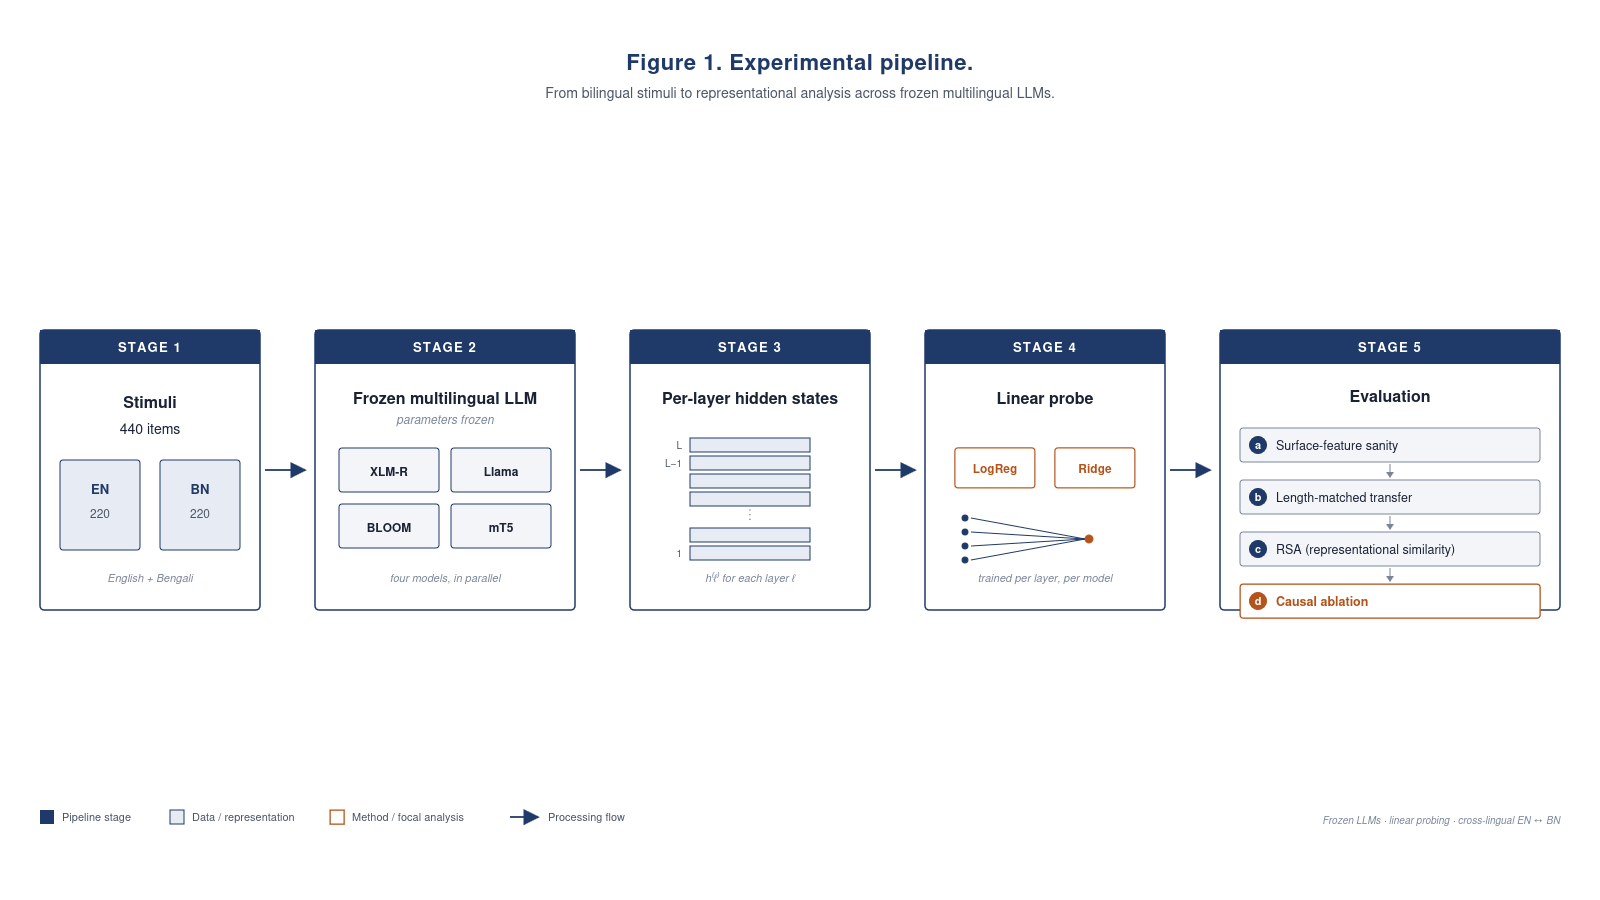
\includegraphics[width=0.95\textwidth]{fig_pipeline.png}
\caption{End-to-end probing pipeline. The 440-stimulus English/Bangla dataset is fed through each frozen multilingual LLM (XLM-R, Llama, BLOOM, mT5); per-layer hidden states are extracted, a linear probe (LogReg/Ridge) is trained, and the resulting representations are evaluated under surface-feature sanity checks, length-matched cross-lingual transfer, Representational Similarity Analysis and causal forward-hook ablation.}
\label{fig:methodology-pipeline}
\end{figure}

\section{Preliminary Design or Design (Model) Specification}

Three design alternatives were considered before settling on frozen per-layer linear probing.

\textbf{Alternative A: Fine-tune each model on each task.} Highest expected performance, but conflates model knowledge with task-specific adaptation, requires large labelled corpora that do not exist for Bangla phonology, and is roughly $10^{6}$ times more expensive in compute than frozen probing. Rejected.

\textbf{Alternative B: Single-layer (final hidden state) probing.} Standard practice in some sentence-level probing studies, but discards information about \emph{where} a feature emerges in the network and prevents the layer-emergence comparison plot (Figure~\ref{fig:layer-emergence}). Rejected.

\textbf{Alternative C (selected): Per-layer linear probing with surface-feature baselines and causal ablation.} Frozen models, linear probes (logistic regression for classification, ridge for regression), per-layer evaluation, length-matched stimulus subsets, RSA and forward-hook ablation. This alternative isolates representational content from model behaviour, exposes layer-wise emergence, and supports causal-localisation claims via random-unit controls. Selected.

\subsection{Models and architectural specification}

Table~\ref{tab:model-specs} summarises the four probed models.

\begin{table}[H]
\centering
\caption{Architectural specification of the four probed multilingual LLMs.}
\label{tab:model-specs}
\small
\resizebox{\textwidth}{!}{%
\setlength{\tabcolsep}{10pt}
\renewcommand{\arraystretch}{2}
\begin{tabular}{|c|c|c|c|c|c|}
\hline
\textbf{Model} & \textbf{Architecture} & \textbf{Tokeniser} & \textbf{Layers} & \textbf{Hidden} & \textbf{Bangla coverage} \\
\hline
XLM-R large    & encoder-only         & SentencePiece     & 24            & 1024 & explicit \\
\hline
Llama 3.1 8B   & decoder-only         & tiktoken BPE      & 32            & 4096 & minimal \\
\hline
BLOOM 7B1      & decoder-only         & BPE               & 30            & 4096 & explicit (ROOTS) \\
\hline
mT5 XL         & encoder-decoder      & SentencePiece     & 24 (encoder)  & 2048 & explicit \\
\hline
\end{tabular}%
}
\end{table}

For mT5 XL only the encoder is probed; the decoder is held frozen and not used for representation extraction. Figure~\ref{fig:model-architectures} compares the four architectures side by side.

\begin{figure}[H]
\centering
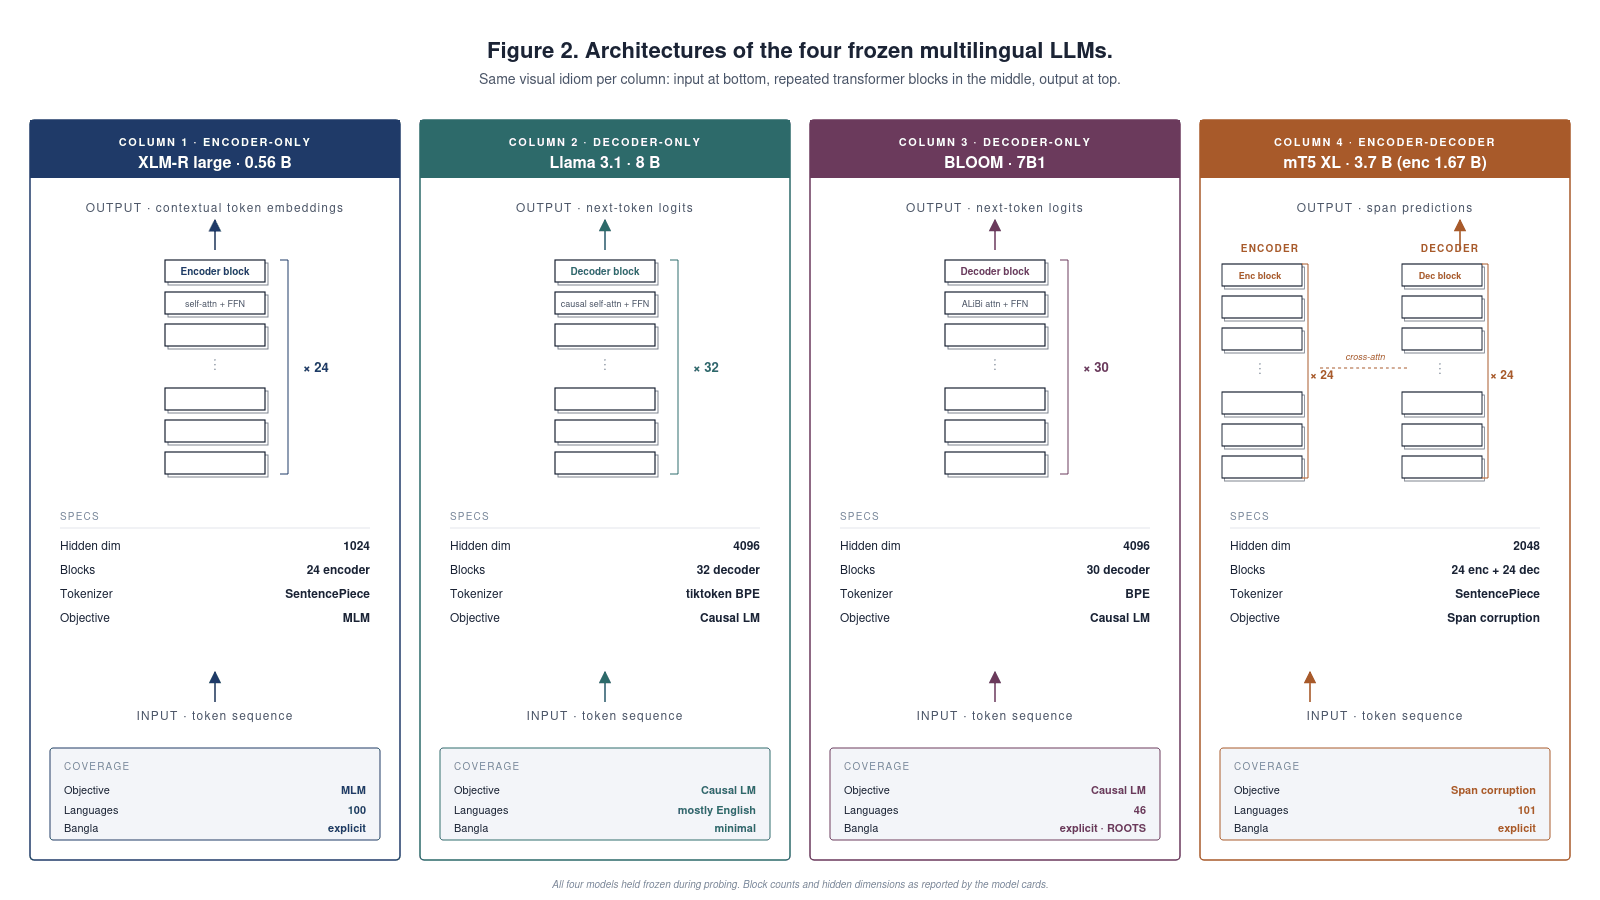
\includegraphics[width=0.98\textwidth]{fig_models.png}
\caption{Side-by-side comparison of the four probed multilingual LLM architectures. XLM-R large is an encoder-only multilingual masked language model; Llama 3.1 8B is an English-heavy causal decoder; BLOOM 7B1 is a 46-language causal decoder with explicit Bangla coverage; mT5 XL is a 101-language span-corruption encoder-decoder. Layer count, hidden size, tokeniser and Bangla coverage are annotated per column.}
\label{fig:model-architectures}
\end{figure}

The four models were selected to exhaust the four canonical pretraining recipes in multilingual NLP as of 2024: a multilingual masked encoder, an English-heavy causal decoder, a multilingual causal decoder, and a multilingual span-corruption encoder-decoder. The following subsections describe each model individually, focusing on the design choices that are most relevant to cross-lingual lexical probing.

\subsection{XLM-RoBERTa large}

XLM-RoBERTa large \cite{conneau2020xlmr} is a 0.56-billion-parameter encoder-only Transformer trained with masked language modelling (MLM) on a 100-language version of the CommonCrawl corpus (CC-100). The model uses a 24-layer encoder stack with hidden dimension 1024 and a SentencePiece tokeniser with a 250{,}000-token vocabulary built jointly across all 100 pretraining languages. Bangla is present in the pretraining mix as an explicitly covered language, and SentencePiece allows Bangla conjunct characters (\textit{yuktoborno}) to be tokenised into subword units rather than discarded. The MLM objective forces the encoder to learn bidirectional contextual representations that integrate information from both left and right context at every position, which is the standard substrate for downstream cross-lingual probing studies \cite{conneau2018probing,hewitt2019structural}. XLM-R large is included here as the representative multilingual MLM-encoder; it is also the smallest model in the comparison, which lets the study quantify how much of cross-lingual lexical transfer can be attributed to multilingual pretraining objective independent of scale.

\textbf{How it works in this study.} Each stimulus (an isolated English or Bangla word) is fed to the model as a single sequence consisting of \texttt{<s>}, the SentencePiece-tokenised word and \texttt{</s>}. A single forward pass in evaluation mode (\texttt{model.eval()}, \texttt{torch.no\_grad()}) returns the 24 layers of hidden states. For each layer the per-token states are mean-pooled across all non-special tokens to a single 1024-dimensional vector, producing a 24-by-1024 representation matrix per stimulus. These vectors are cached to disk under \texttt{Dyslexia-XLM-R/representations/} and consumed by the per-layer probes in the next stage. Because XLM-R is bidirectional, the same forward pass yields representations regardless of token position; no causal-mask correction is needed. The model fits in 16-bit precision on a single 24~GB consumer GPU with no quantisation. Implementation: \texttt{Dyslexia-XLM-R/main.ipynb}.

\subsection{Llama 3.1 8B}

Llama 3.1 8B \cite{dubey2024llama3} is an 8-billion-parameter decoder-only autoregressive Transformer with 32 decoder layers and hidden dimension 4096, trained with a causal language modelling objective on a predominantly English corpus. The tokeniser is a tiktoken-style byte-pair encoding tuned for English with limited explicit coverage of Indic scripts; Bangla characters are handled at the byte level, which is functional but does not group conjuncts as semantic units. Llama 3.1 is the largest and most recent open-weight causal decoder used in this study and represents the dominant industrial recipe of 2024, namely scale-up of a primarily English causal LM. Including it in the comparison is essential precisely because its multilingual coverage is minimal: if any of the cross-lingual lexical signal in this study reflected pure model scale rather than pretraining language coverage, it would surface most clearly in Llama.

\textbf{How it works in this study.} The model is loaded with 4-bit weight quantisation via Unsloth and bitsandbytes \cite{dettmers2022bnb} so that all 32 decoder layers fit on a single 24~GB consumer GPU; activations remain in 16-bit. Each stimulus is fed through the model as a single sequence preceded by the Llama beginning-of-sequence token, with no prompt template. A causal forward pass in evaluation mode yields the 32 layers of hidden states; the causal attention mask means that the state at token position $t$ is conditioned only on tokens up to $t$, so the last token always carries the richest summary in autoregressive use. For consistency with the encoder-based models, however, hidden states for each layer are mean-pooled across all input tokens (excluding the beginning-of-sequence token), producing a 32-by-4096 representation matrix per stimulus. This choice is justified by the probing literature, which finds that mean pooling of decoder hidden states yields more robust linear-probe accuracy than last-token pooling when the downstream task is classification over isolated tokens \cite{conneau2018probing}. Representations are cached under \texttt{dyslexia-LLM/representations/}. Implementation: \texttt{dyslexia-LLM/main.ipynb}.

\subsection{BLOOM 7B1}

BLOOM 7B1 \cite{scao2022bloom} is a 7.1-billion-parameter decoder-only autoregressive Transformer with 30 decoder layers and hidden dimension 4096, trained with a causal language modelling objective on the ROOTS corpus, an explicitly multilingual collection covering 46 natural languages with deliberate over-sampling of low-resource and South-Asian languages including Bangla. The tokeniser is a BPE tokeniser trained jointly across all 46 languages, which means Bangla subword units are first-class citizens of the vocabulary rather than being decomposed at the byte level. BLOOM 7B1 is included as the representative multilingual causal decoder; its pairing with Llama 3.1 8B is the cleanest possible test of whether \emph{multilingual} pretraining of a causal decoder produces transferable cross-lingual lexical structure, because the two models share architecture family and operate at similar parameter scale and differ primarily in pretraining language coverage.

\textbf{How it works in this study.} The pipeline mirrors the Llama pipeline so that any difference in measured cross-lingual transfer is attributable to the pretraining recipe rather than to instrumentation. BLOOM is loaded with 4-bit weight quantisation via Unsloth and bitsandbytes for GPU memory feasibility, with activations in 16-bit. Each stimulus is fed as a single sequence with no prompt template; a single causal forward pass returns the 30 layers of hidden states. Per-layer mean pooling across input tokens (excluding the beginning-of-sequence token) produces a 30-by-4096 representation matrix per stimulus, cached to \texttt{dyslexia-bloom/representations/}. Because BLOOM's BPE tokeniser was trained jointly on Bangla, Bangla input strings decompose into meaningful subword units rather than into raw bytes, and the per-layer mean pool is therefore taken over a smaller and more semantically coherent token sequence than the Llama equivalent. Implementation: \texttt{dyslexia-bloom/main.ipynb}.

\subsection{mT5 XL}

mT5 XL \cite{xue2021mt5} is a 3.7-billion-parameter encoder-decoder Transformer (1.67-billion-parameter encoder) trained with a T5-style span-corruption objective on a 101-language version of the C4 corpus (mC4). The encoder has 24 layers with hidden dimension 2048 and uses a SentencePiece tokeniser shared with the decoder. Bangla is explicitly covered. Span-corruption masks contiguous spans of input tokens and trains the decoder to regenerate them; this objective is qualitatively different from both MLM (which masks individual tokens and reads them off bidirectional context) and causal LM (which never sees right-context at training time), and the resulting encoder representations are organised differently. Critically for this thesis, mT5 is the only encoder-decoder model in the comparison; if the cross-lingual lexical signal turns out to localise differently in mT5 than in the three encoder-only or decoder-only models, the result is interpretable as a property of either the span-corruption objective or the encoder-decoder split, and this is flagged explicitly in the limitations.

\textbf{How it works in this study.} Only the encoder is used. Each stimulus is tokenised with the shared SentencePiece tokeniser and passed through the encoder in evaluation mode; the decoder is loaded but is never invoked during representation extraction. A single forward pass yields the 24 encoder-layer hidden states; per-layer mean pooling over the input tokens produces a 24-by-2048 representation matrix per stimulus, cached to \texttt{dyslexia-mt5/representations/}. The encoder is bidirectional like XLM-R's, so no causal-mask correction is needed. Because the encoder is only 1.67B parameters, mT5 XL fits in 16-bit precision on a single 24~GB consumer GPU without quantisation, which makes mT5 the most expensive but also the highest-fidelity model in the study and is the reason the depth-scan ablation (five \texttt{measure\_L} values, three random-unit seeds each) is run on mT5 specifically and not on the larger BLOOM and Llama decoders. Implementation: \texttt{dyslexia-mt5/main.ipynb}.

\subsection{Why these four}

Each of the four models is the strongest publicly released representative of its pretraining recipe that runs on a single consumer GPU under 4-bit quantisation. Together they span the two-by-two design grid that defines the multilingual LLM landscape in 2024: \{\emph{encoder-only, decoder-only, encoder-decoder}\} crossed with \{\emph{multilingual, English-heavy}\}. Comparing them on the same surface-controlled stimuli with the same probes is the minimal experimental design that lets the thesis make claims about which pretraining recipe carries cross-lingual lexical structure. The four-model comparison is also a precondition for the model-selection recommendation in Chapter~6: without all four families on the same evaluation, it would not be possible to argue that BLOOM is the best practical substrate for a low-resource Bangla screening prototype and that mT5 is the best interpretability substrate.

\section{Data Collection}

\subsection{Stimulus dataset}

The dataset is a single CSV (\texttt{dyslex\_probe\_stimuli\_clean.csv}, 440 rows, 18 columns) committed to each per-model repository. It covers 220 English and 220 Bangla items across seven task categories: minimal pair (60 per language), multisyllabic (30), pseudoword (25), real word (25), phoneme-grapheme (25), rhyme (20) and sentence (15). The detailed per-category counts and the eighteen-column schema are reproduced in Appendix~B.

The Bangla side of the stimulus design is grounded in the Master's dissertation work of Badsha \cite{badsha2024mall}, who documented the phonological difficulty patterns of five dyslexic Bangla-speaking primary-school children at the University of Dhaka and published the consolidated findings in IJFMR (vol.\ 6, no.\ 3, May-June 2024). Three elements of our stimulus design are taken directly from that work: (i) the five voiced/unvoiced stop pairs ({\banglafont ক/গ}, {\banglafont প/ব}, {\banglafont ত/দ}, {\banglafont ট/ড}, {\banglafont চ/জ}) used as the Bangla minimal-pair category, (ii) the multisyllabic-word and \textit{matra} error patterns that informed the multisyllabic category, and (iii) the human difficulty ranking (voicing hardest to syllable-count easiest) against which we later compare the four-model ablation pattern in Chapter~5.

Bangla items are stored in Unicode Bengali script with author-assigned IPA, syllable count, phonological complexity, orthographic transparency, voiced/unvoiced label, real-word flag, consonant-cluster flag and irregular-mapping flag. All Bangla items were inspected by a native Bangla speaker for orthographic validity; flagged items were revised or replaced. Bangla pseudowords were generated to follow Bangla phonotactic patterns and re-checked to remove accidental real words.

\subsection{Probing labels}

For each task the label set is:
\begin{itemize}
    \item \textbf{Voicing}: binary \{voiced, unvoiced\}, used on minimal-pair and real-word items where the leading stop consonant has a clear voicing class.
    \item \textbf{Real vs.\ pseudo word (``realword'')}: binary \{real, pseudo\}, used on the union of the real-word and pseudoword categories.
    \item \textbf{Orthographic transparency (``ortho'')}: binary \{transparent, opaque\}, assigned per item from orthographic-mapping rules.
    \item \textbf{Syllable count}: integer regression target.
\end{itemize}

\subsection{Data Cleaning}

Tokeniser-level normalisation differs across model families. To avoid biasing length-based controls, all length statistics (character length, byte length, unique-character count, vowel ratio, consonant-run length) are computed on the original Unicode string before tokenisation, not on the tokeniser output. Bangla conjunct characters (\textit{yuktoborno}) are preserved in their default Unicode encoding; the surface-feature baseline uses the original-string statistics, not the model's subword decomposition.

\subsection{Data Transformation}

For each stimulus the model returns a per-layer sequence of hidden states. For word-level items the per-token states are mean-pooled across the token sequence to a single fixed-dimensional vector per layer per item; for the encoder-decoder model the mean pool is taken over encoder token states only. No normalisation is applied to the pooled vector; probes are trained on the raw pooled hidden state, which is standard in the probing literature \cite{conneau2018probing}.

\subsection{Data Integration}

The hidden-state cache is stored per model in the \texttt{representations/} subdirectory of each per-model repository (one tensor per layer per language). Results from independent model runs are integrated downstream into the comparison files (\texttt{comparison\_three\_models.md} and \texttt{comparison\_four\_models.md}/.xlsx) by joining on (task, layer) keys.

\subsection{Data Reduction}

For the length-matched probing pass (Section~\ref{sec:rq2}), the real-word and pseudoword subsets are reduced to 50 matched pairs per language by selecting 1:1 character-length matches. Mean character length within the matched English subset is 6.88 characters; within the matched Bangla subset, 5.20 characters. This subset is the only one on which length-matched cross-lingual transfer numbers are reported.

\subsection{Summary of Preprocessed Data}

The final analysis-ready dataset is the 440-item stimulus CSV, the per-layer hidden-state caches (one per model), the four label vectors (voicing, realword, ortho, syllable), the 100-item length-matched realword subset (50 EN + 50 BN), and the five-feature character-statistic baseline matrix used in the sanity-check pass.

\section{Implementation of Selected Design}

The full software stack (Python 3.10, PyTorch, Hugging Face \texttt{transformers}, \texttt{scikit-learn}, Unsloth, bitsandbytes, \texttt{matplotlib}, \texttt{pandas} and the pinned version numbers used in this study) and the full hardware specification (single NVIDIA consumer GPU with 24~GB VRAM; 4-bit quantisation for the 7--8B causal decoders) are enumerated in \textbf{Appendix~A: Tools, Software, Hardware and Reproducibility}. The implementation subsections below describe how the design of Chapter~4 is realised in code; readers seeking the exact tool versions, environment files, random seeds and reproducibility checklist should refer to Appendix~A.

\subsection{Representation extraction}

For each model, a single Python notebook loads the frozen pretrained weights via Hugging Face \texttt{transformers}, performs one forward pass per stimulus and writes per-layer mean-pooled hidden states to disk. The Llama and BLOOM models are loaded in 4-bit precision via Unsloth + bitsandbytes \cite{dettmers2022bnb}; XLM-R large and the mT5 encoder fit in 16-bit on a single 24~GB consumer GPU. No model parameters are updated; \texttt{model.eval()} and \texttt{torch.no\_grad()} are enforced throughout.

\subsection{Per-layer probing}

For each (model, layer, task) tuple a fresh probe is trained: L2-regularised logistic regression (scikit-learn, default $C=1.0$) for the three classification tasks, ridge regression (default $\alpha=1.0$) for syllable count. The English subset is split 80/20 (stratified for classification) with \texttt{random\_state=42}. The English-trained probe is evaluated on the held-out English test split (in-language metric) and on the entire Bangla subset (zero-shot cross-lingual transfer metric). Reported metrics are macro F1 for classification and $R^2$ for regression, both averaged over a 5-fold cross-validation within the English training split for layer-selection robustness. Figure~\ref{fig:probing-schematic} illustrates the per-layer probing setup.

\begin{figure}[H]
\centering
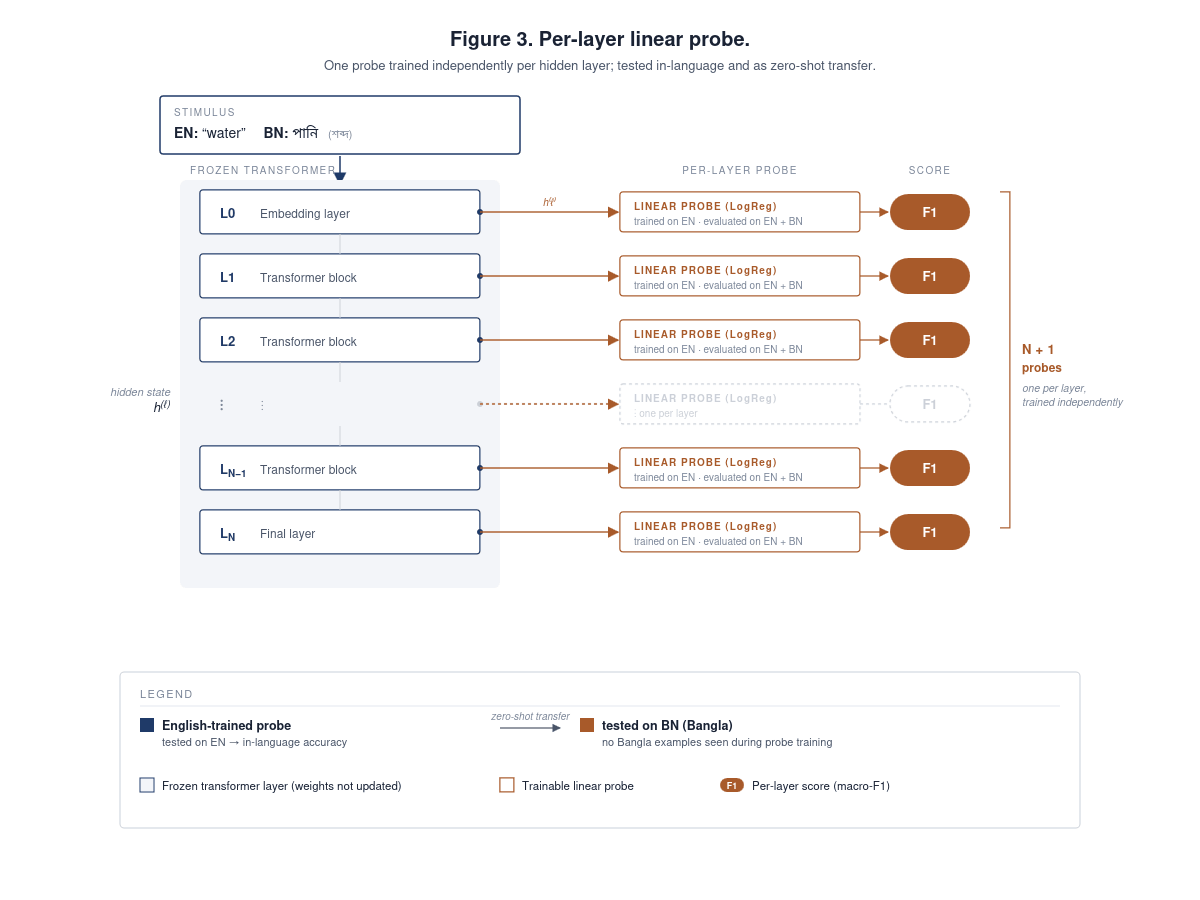
\includegraphics[width=0.85\textwidth]{fig_probing.png}
\caption{Per-layer linear probing schematic. A stimulus passes through the frozen model; each layer's mean-pooled hidden state feeds a separately trained linear probe. The English-trained probe is then evaluated on held-out English (in-language) and on the full Bangla subset (zero-shot cross-lingual transfer).}
\label{fig:probing-schematic}
\end{figure}

\subsection{Surface-feature sanity checks}

Three sanity-check baselines are run.

\textbf{First-character lookup (voicing).} For each Bangla voicing label, the leave-one-out probe is trained on the layer-0 (token-embedding) hidden state with a one-hot encoding of the first character. The resulting F1 quantifies how much voicing information is recoverable from the first character alone (Section~\ref{sec:sanity}, Figure~\ref{fig:bn-voicing-sanity}).

\textbf{Five-feature character-statistic baseline (ortho, syllable).} A logistic / ridge baseline is trained on five hand-crafted features per item: character length, byte length, unique-character count, vowel ratio, longest consonant run. The baseline is run separately for English and Bangla. Any LLM probe whose F1 / $R^2$ does not exceed this baseline by more than 0.03 is interpreted as not contributing information above surface statistics.

\textbf{Length matching (realword).} Real and pseudo word items are matched 1:1 on character length within each language. Probes trained on the matched subset are reported as the only surface-controlled realword numbers.

\subsection{Representational Similarity Analysis}

For each (model, layer) the Representational Dissimilarity Matrix (RDM) over the 220 same-language items is computed using $1 - \cos\theta$ on the mean-pooled hidden states. The English RDM and the Bangla RDM are compared by Spearman $\rho$ on their flattened upper triangles; a high $\rho$ at a layer indicates preserved cross-lingual representational geometry. The mate-retrieval Top-1 accuracy (given an English item, retrieve the matched Bangla item by minimum-cosine-distance) is computed in parallel.

\subsection{Causal forward-hook ablation}

For the length-matched realword task, a probe is first trained on the English baseline at the chosen \texttt{measure\_L} layer (the layer at which transfer is measured). A forward hook is then registered three layers earlier (\texttt{measure\_L - 3}) that, during the forward pass, zeros a chosen subset of hidden units. Two ablation conditions are compared: \textbf{top-$K$} (the $K$ units with the largest absolute probe weights) and \textbf{random-$K$} (a random subset of $K$ units, averaged over three random seeds). The drop in Bangla F1 is reported per condition; \emph{ablation specificity} is defined as (\text{baseline} $-$ \text{top-$K$ accuracy}) $-$ (\text{baseline} $-$ \text{random-$K$ accuracy}). For most reported numbers $K=20$ at the four-model level and $K=10$ at the mT5 depth-scan level. Figure~\ref{fig:ablation-schematic} summarises the design.

\begin{figure}[H]
\centering
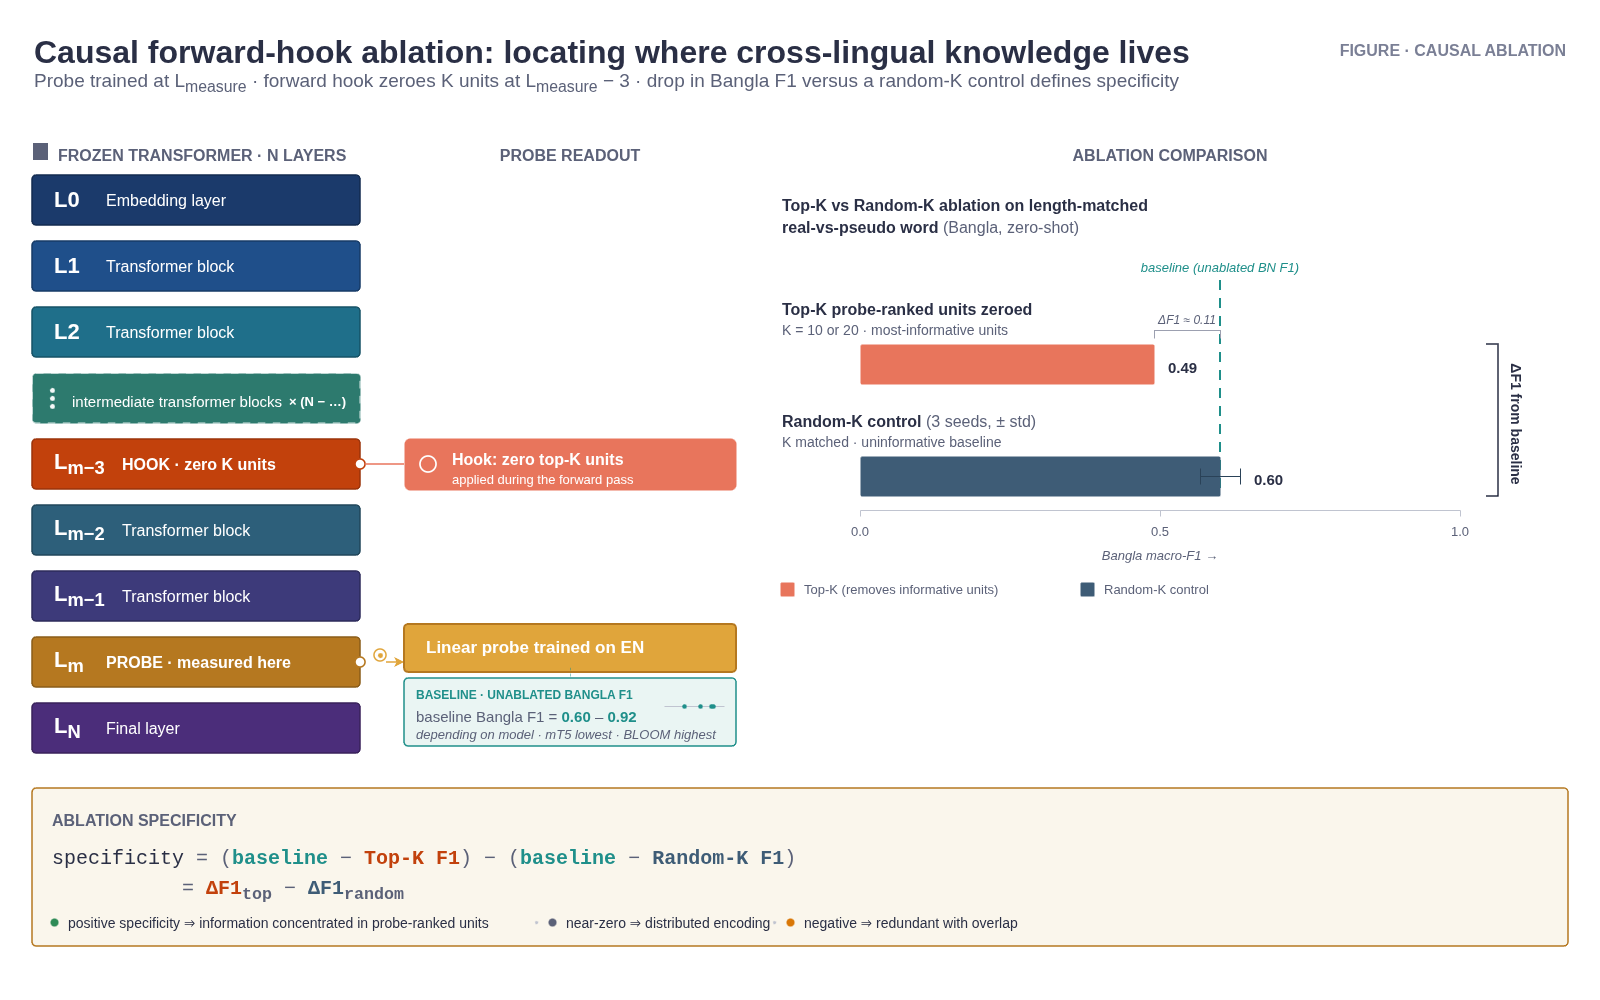
\includegraphics[width=0.95\textwidth]{fig_ablation.png}
\caption{Causal forward-hook ablation. The probe is trained at \texttt{measure\_L}; a forward hook three layers earlier zeros either the top-$K$ probe-ranked units or a random-$K$ control. The drop in Bangla F1 versus the random-$K$ control defines ablation specificity; a positive specificity indicates concentrated, causally relevant units.}
\label{fig:ablation-schematic}
\end{figure}

\subsection{mT5 depth-scan and unit-overlap analysis}

The mT5 encoder ablation is repeated at five depths (\texttt{measure\_L} $\in$ \{4, 8, 12, 16, 20\}) with three random seeds per depth. At each depth the top-10 probe-ranked units are recorded; the pairwise Jaccard overlap of the top-10 sets across depths is then tabulated. A unit that appears in the top-10 at three or more depths is reported as a \emph{persistent backbone} unit; in the mT5 encoder these are u782 and u1880. The analysis answers two questions: (i) does localisation persist across depth or is it specific to one layer; (ii) are the same units carrying the information across depths or does each depth use a layer-local set. Figure~\ref{fig:mt5-backbone-schematic} previews the expected hybrid pattern that the depth-scan ultimately confirms in Chapter~5.

\begin{figure}[H]
\centering
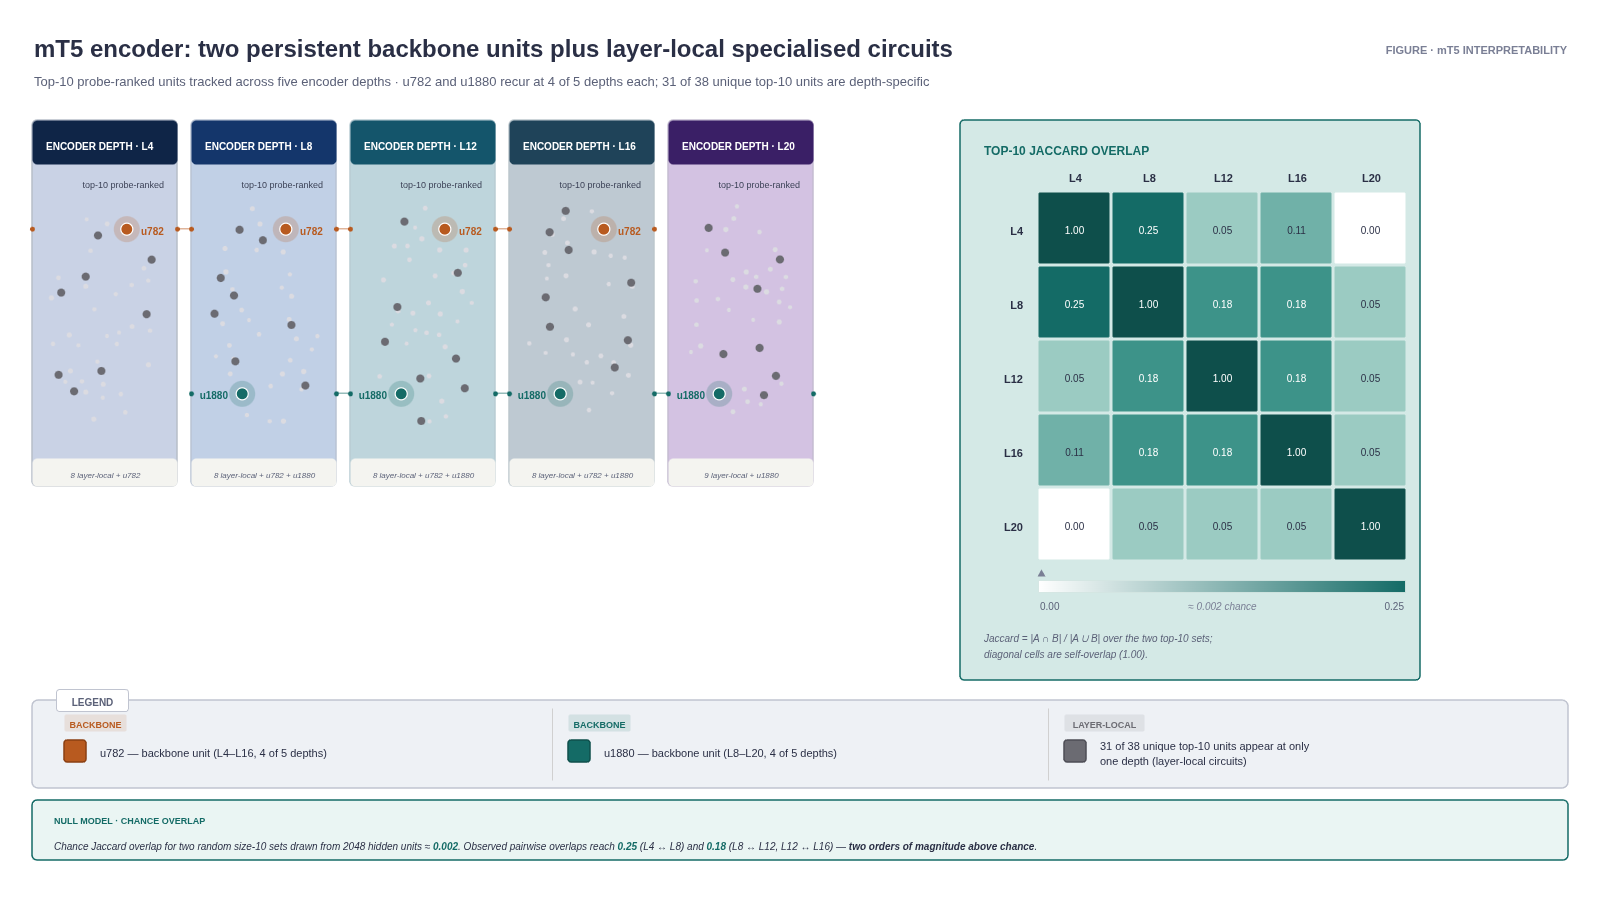
\includegraphics[width=0.95\textwidth]{fig_mt5_backbone.png}
\caption{Schematic of the hybrid backbone-plus-routing pattern probed in the mT5 encoder. Two units (u782, u1880) appear in the top-10 probe-ranked set across four of the five probed encoder depths and constitute a persistent backbone; the remaining top-10 units at each depth are layer-local specialised circuits.}
\label{fig:mt5-backbone-schematic}
\end{figure}

\subsection{Reproducibility}

Every result table in Chapter~5 corresponds to a deterministic CSV in the per-model results directory: \texttt{results\_english\_probing\_*.csv}, \texttt{results\_transfer\_*.csv}, \texttt{results\_rsa\_*.csv}, \texttt{results\_ablation\_*.csv}, \texttt{results\_*\_realword\_matched.csv} and (for mT5) \texttt{results\_mt5\_localization\_depth\_scan.csv} and \texttt{results\_mt5\_unit\_overlap.csv}. Random seeds, scikit-learn versions and CUDA versions are pinned in Appendix~A. The four-model integration is emitted to \texttt{comparison\_four\_models.md} and \texttt{comparison\_four\_models.xlsx} in \texttt{dyslexia-mt5/}.


\chapter{Result Analysis}
\section{Performance Evaluation}
\label{sec:perf-eval}

\subsection{Evaluation criteria and reporting conventions}

Probe performance is reported with macro-F1 for the three classification tasks (voicing, real vs.\ pseudo word, orthographic transparency) and with the coefficient of determination $R^2$ for the syllable-count regression task. Reported per-model numbers are the peak across all model layers; layer-emergence figures show the full per-layer trajectory. In-language scores are computed on a held-out English split (80/20, stratified, fixed seed 42); cross-lingual scores are zero-shot transfer to the Bangla subset using the English-trained probe weights without any Bangla-side fitting. Surface-feature baselines (first-character lookup and a five-feature character-statistic baseline) are reported alongside model scores so that the \emph{gain over surface} judgement that underpins the sanity-check conclusion of Section~\ref{sec:sanity} is explicit at every step.

The chapter answers the four research questions of Section~\ref{sec:rqs} in order. Within Section~\ref{sec:perf-eval}, Section~\ref{sec:rq1} addresses RQ1 (in-language English encoding), Section~\ref{sec:sanity} reports the surface-feature sanity checks that reframe RQ1 and gate everything that follows, Section~\ref{sec:rq2} addresses RQ2 (cross-lingual transfer) on the surface-controlled subset, and Section~\ref{sec:rsa} reports Representational Similarity Analysis as a probe-free corroboration of RQ2. Section~\ref{sec:analysis} (Analysis of Design Solutions) then addresses RQ3 (mechanism and localisation) via causal forward-hook ablation and extends it to a depth-and-overlap analysis on mT5. Section~\ref{sec:adjustments} reports the design adjustments made as a direct consequence of these results, Section~\ref{sec:stats} reports the statistical-analysis conventions, Section~\ref{sec:comparisons} addresses RQ4 (cross-model comparison and model selection) and the relationship to prior work, and Section~\ref{sec:discussion} interprets the joint pattern.

The headline results of the chapter are summarised across the three figures that follow. Figure~\ref{fig:summary-sanity} establishes the surface-feature sanity checks and the length-matched recovery; Figure~\ref{fig:summary-transfer} reports zero-shot cross-lingual transfer and causal-ablation specificity; Figure~\ref{fig:summary-mt5} reports the mT5 localisation analysis. All four model families share the same frozen-LLM pipeline and the same 440-stimulus dataset.

\begin{figure}[H]
\centering
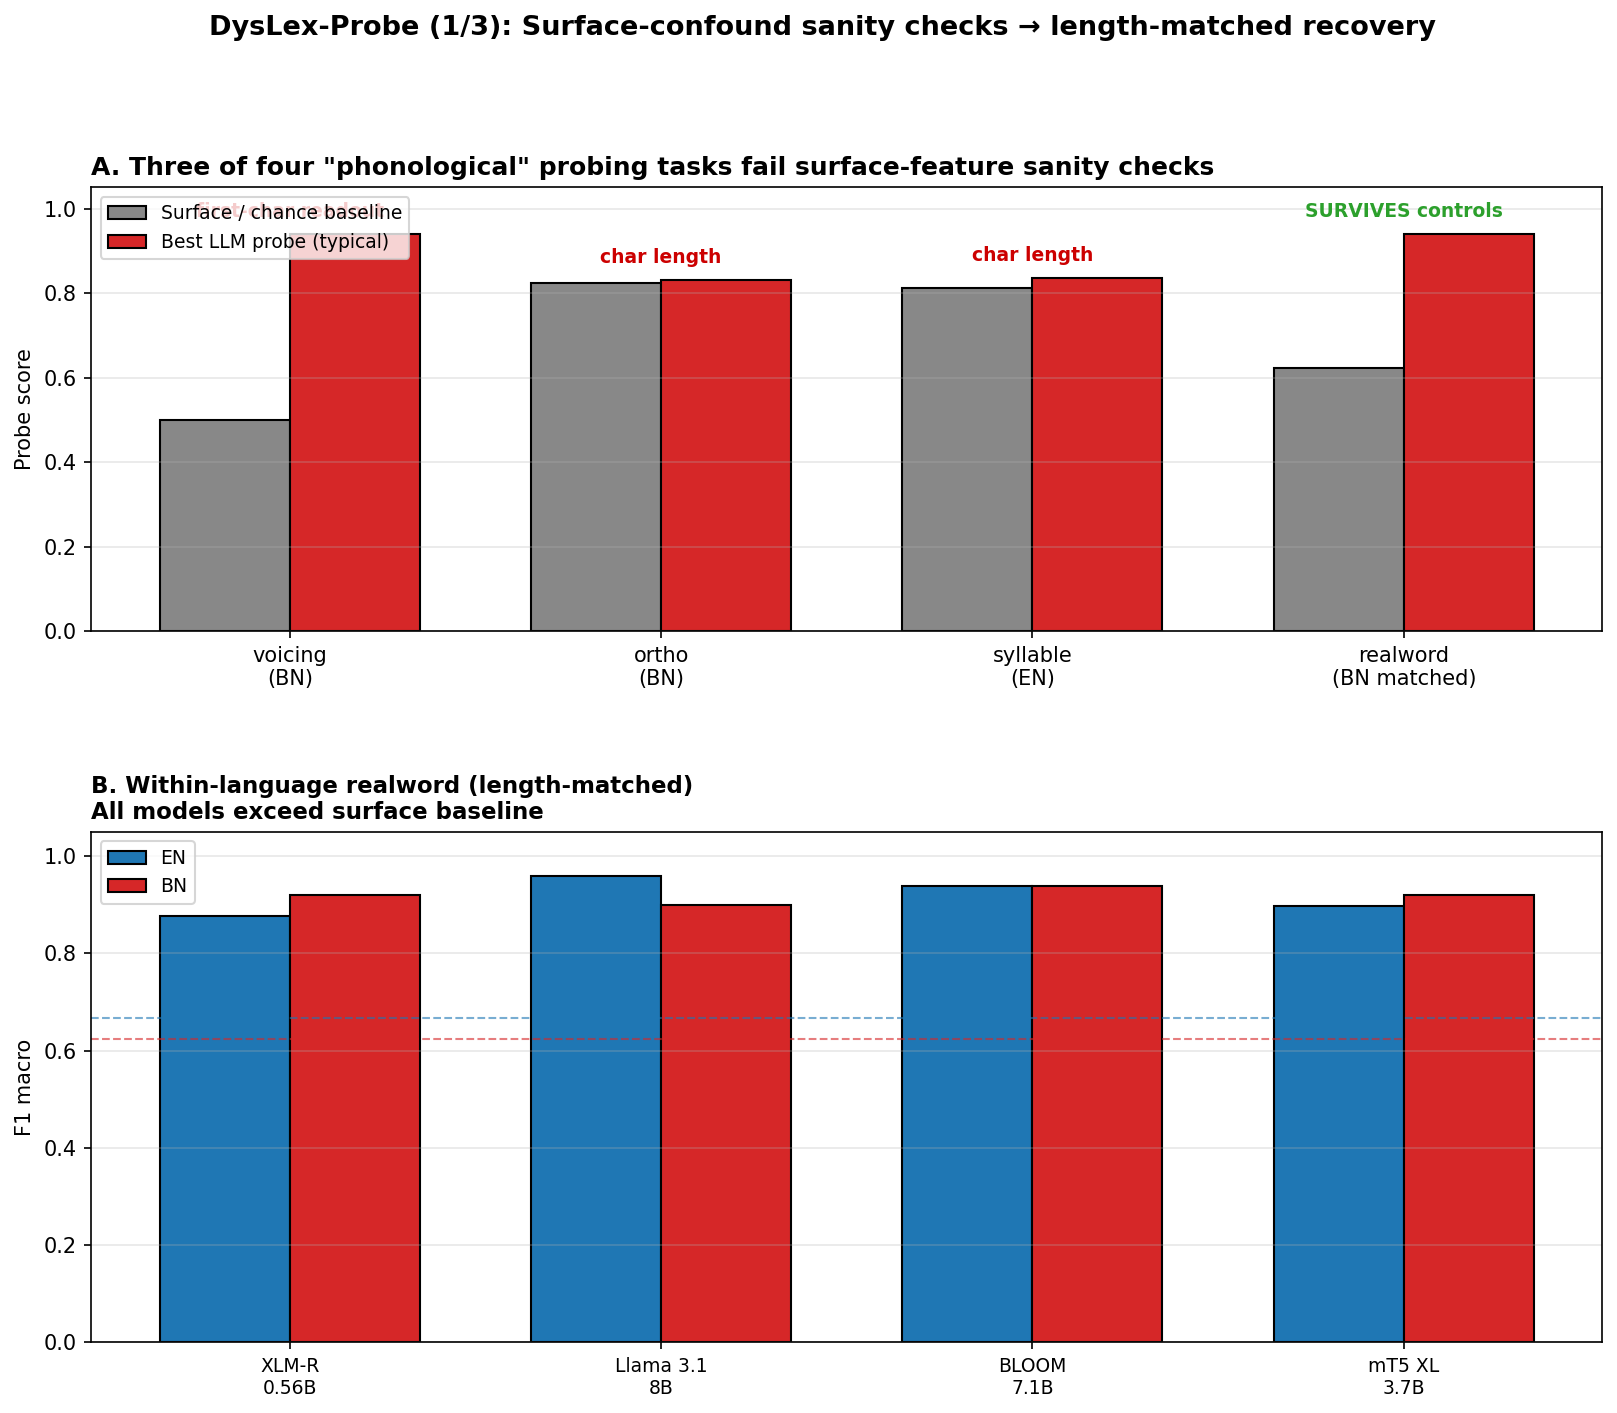
\includegraphics[width=0.95\textwidth]{plots_summary_1_sanity_realword.png}
\caption{Surface-confound sanity checks and length-matched recovery. (A) Three of four ``phonological'' probing tasks fail surface-feature sanity checks; only length-matched real-versus-pseudo word survives. (B) On the length-matched real-word subset, every model exceeds its within-language surface baseline in both English and Bangla.}
\label{fig:summary-sanity}
\end{figure}

\begin{figure}[H]
\centering
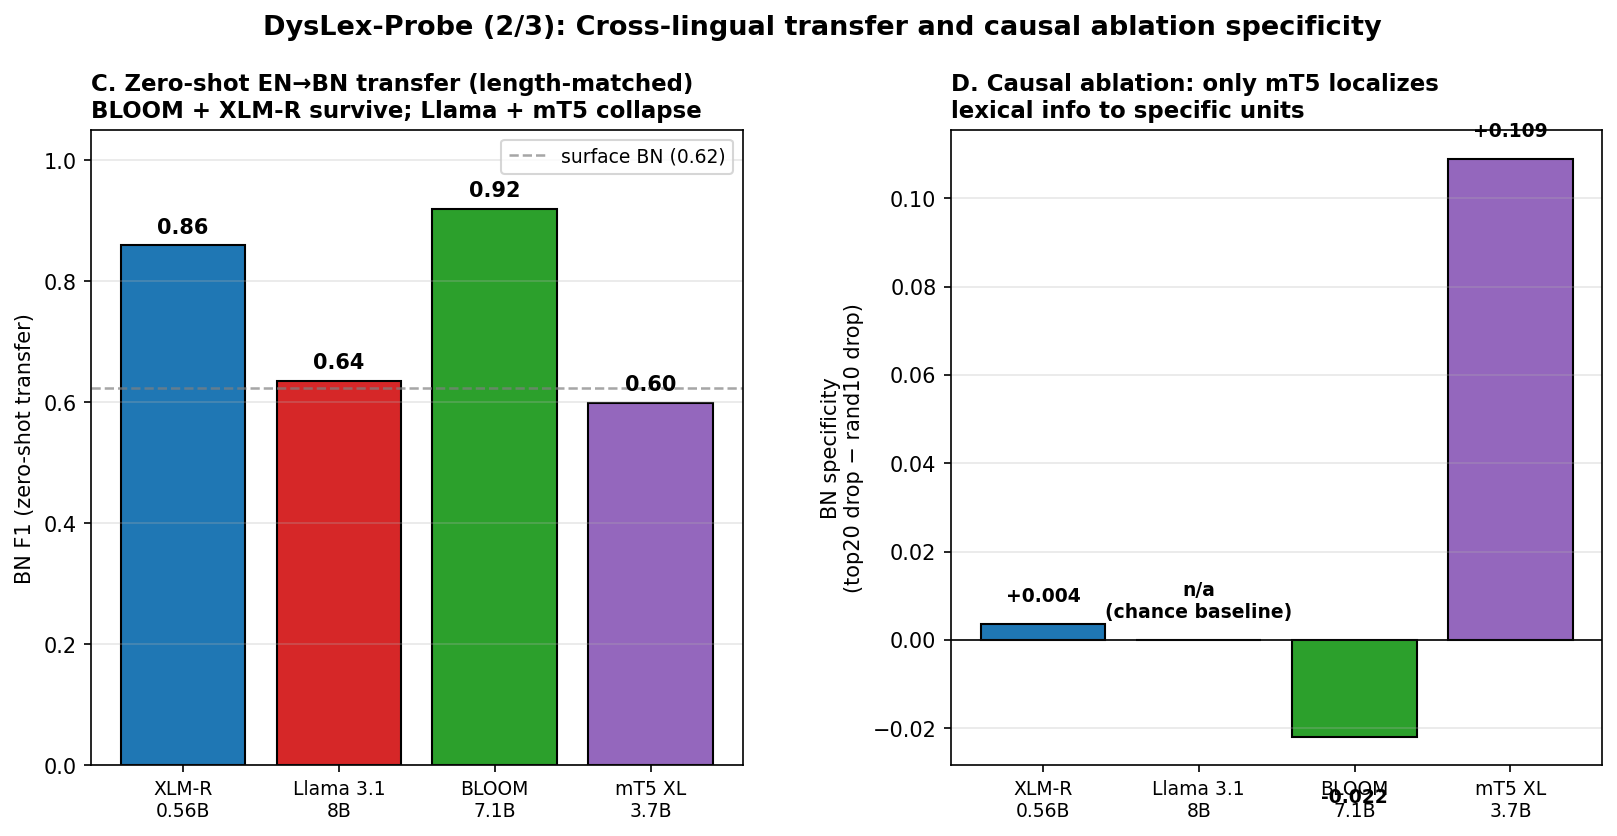
\includegraphics[width=0.95\textwidth]{plots_summary_2_transfer_ablation.png}
\caption{Cross-lingual transfer and causal ablation. (C) Zero-shot English$\rightarrow$Bangla transfer on the length-matched subset: BLOOM and XLM-R survive above the surface baseline, while Llama and mT5 collapse to it. (D) Causal ablation specificity (top-20 drop minus random-10 drop): only mT5 localises lexical information to specific units; Llama is undefined as its baseline sits at chance.}
\label{fig:summary-transfer}
\end{figure}

\begin{figure}[H]
\centering
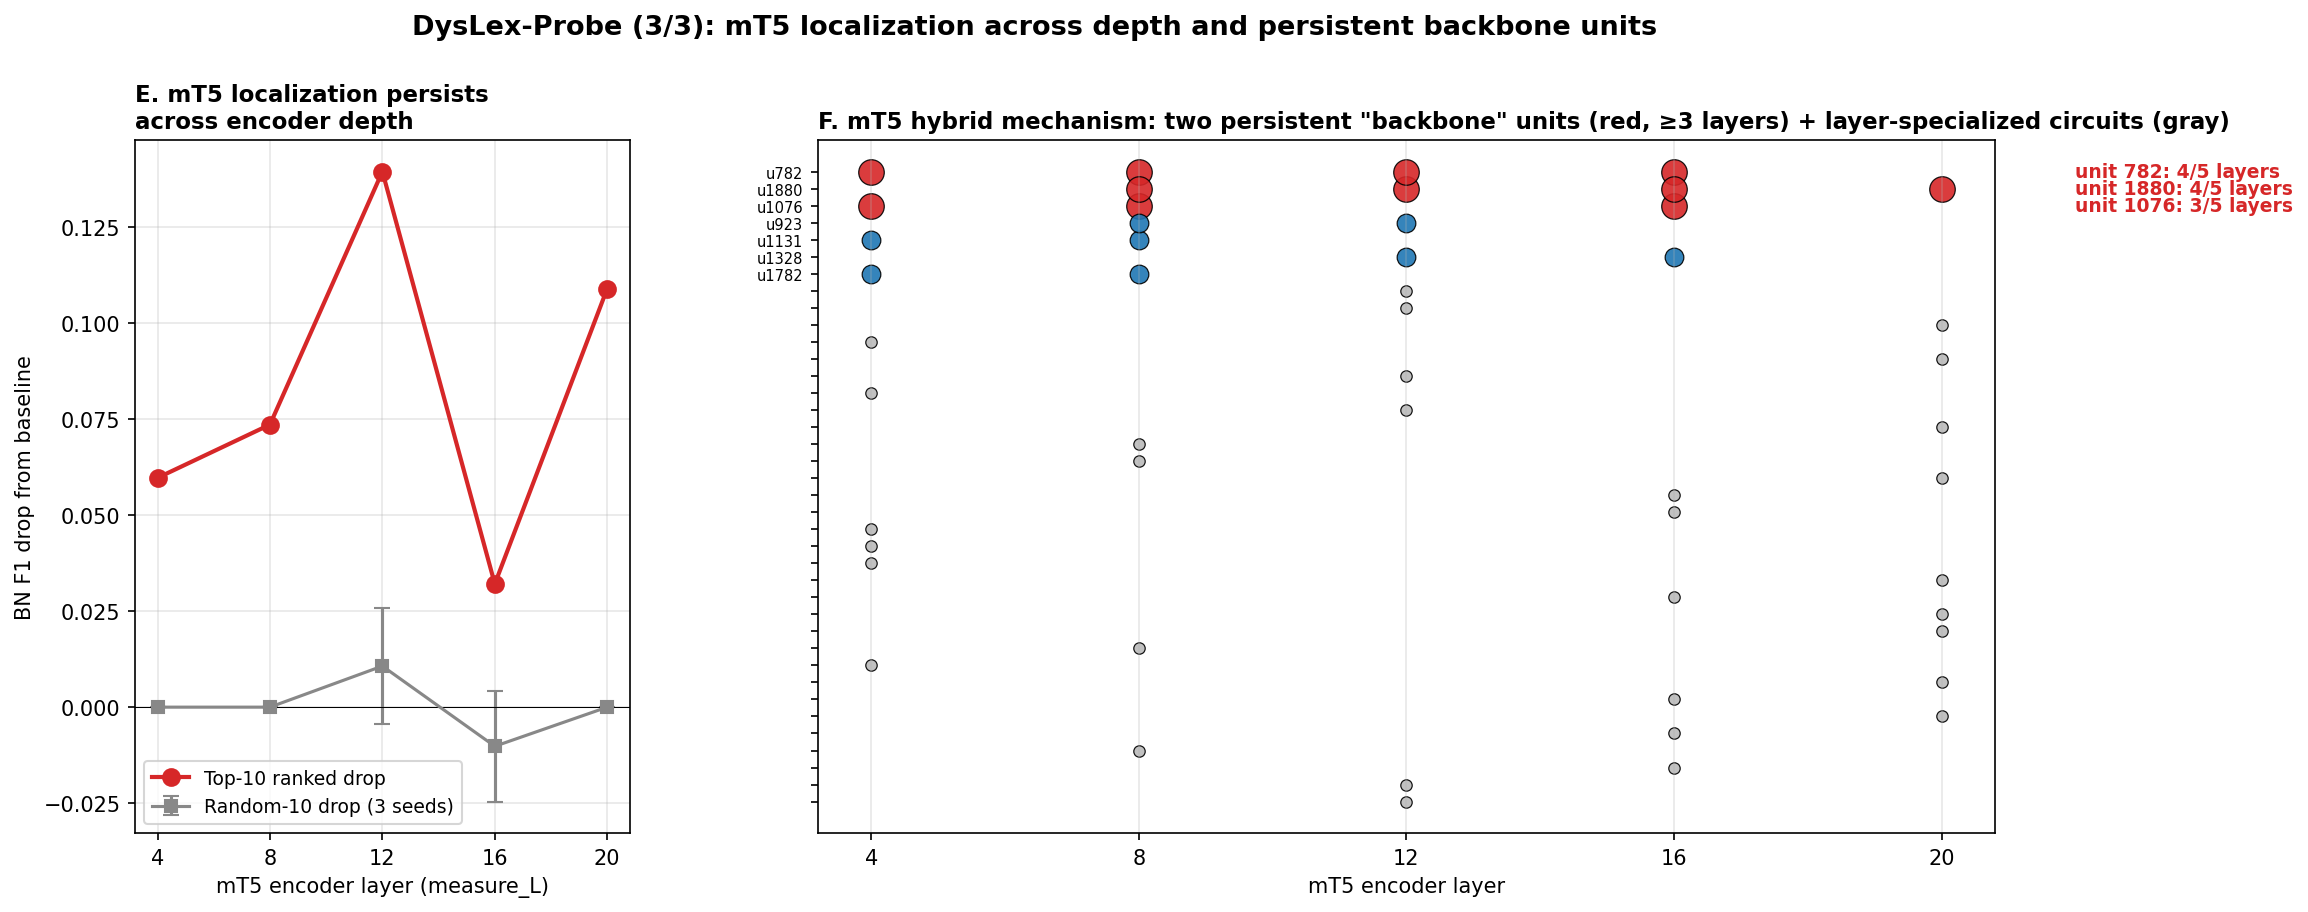
\includegraphics[width=\textwidth]{plots_summary_3_mt5_localization.png}
\caption{mT5 localisation mechanism. (E) The ranked-unit ablation drop exceeds the random-unit drop across encoder depth, so localisation persists rather than being a single-layer artefact. (F) Two persistent ``backbone'' units (red, present in $\geq 3$ of five probed layers) coexist with layer-specialised circuits (gray), indicating a hybrid distributed-plus-localised mechanism.}
\label{fig:summary-mt5}
\end{figure}

\subsection{RQ1: In-language English probing across the four models}
\label{sec:rq1}

Table~\ref{tab:rq1-en} reports per-model peak in-language English performance on the four phonological probing tasks; Figure~\ref{fig:four-english} visualises the per-layer trajectories.

\begin{table}[H]
\centering
\caption{In-language English probing (RQ1): peak layer / peak score per model per task. F1 for voicing, realword, ortho; $R^{2}$ for syllable.}
\label{tab:rq1-en}
\small
\resizebox{\textwidth}{!}{%
\setlength{\tabcolsep}{10pt}
\renewcommand{\arraystretch}{2}
\begin{tabular}{|c|c|c|c|c|}
\hline
\textbf{Task} & \textbf{XLM-R} & \textbf{Llama} & \textbf{BLOOM} & \textbf{mT5} \\
\hline
voicing  & L11 / 0.62 & L2  / 0.73 & L6  / 0.55 & L9  / 0.58 \\
\hline
realword & L11 / 0.84 & L12 / 0.91 & L22 / 0.79 & L24 / 0.81 \\
\hline
ortho    & L0  / 0.92 & L32 / 0.71 & L12 / 0.68 & L21 / 0.69 \\
\hline
syllable & L8  / 0.67 & L16 / 0.70 & L29 / 0.68 & L20 / 0.76 \\
\hline
\end{tabular}%
}
\end{table}

\begin{figure}[H]
\centering
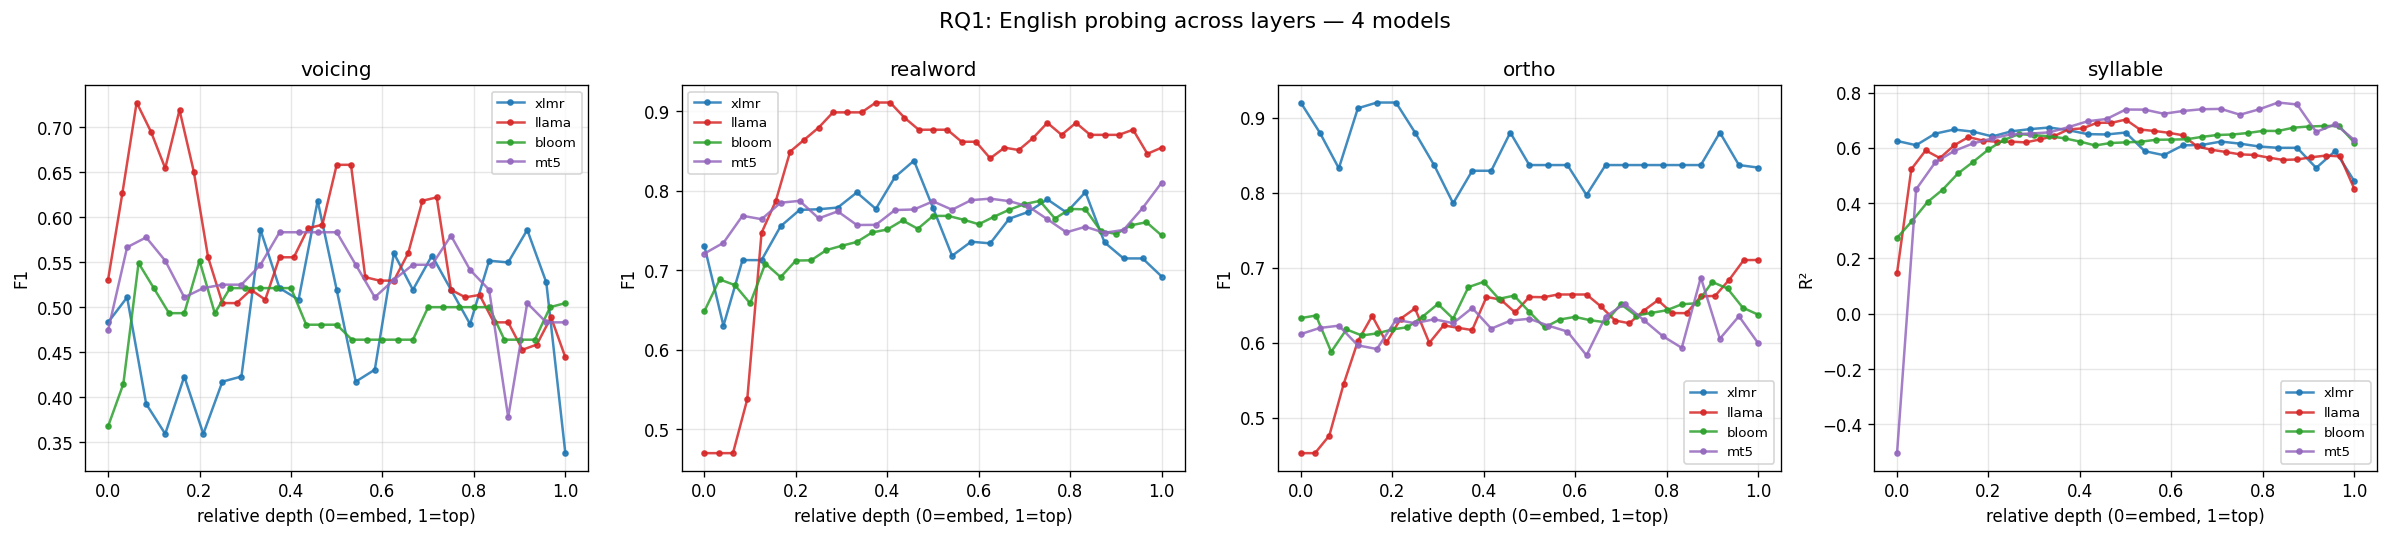
\includegraphics[width=0.95\textwidth]{plots_four_models_english.png}
\caption{Per-layer in-language English probing performance across the four models on voicing, realword, orthographic transparency and syllable count.}
\label{fig:four-english}
\end{figure}

\textbf{Layer-emergence patterns.} The layer-emergence trajectories (Figure~\ref{fig:layer-emergence}) differ across architectures in ways that are interpretable in the light of each model's pretraining objective. XLM-R, the multilingual masked encoder, peaks for the realword task in its middle layers (L11), consistent with prior probing findings that masked encoders concentrate lexical and morphological structure in mid-network and reserve final layers for task-conditional reorganisation \cite{hewitt2019structural,belinkov2022probing}. Llama, the English-causal decoder, peaks early for voicing (L2) and late for syllable count (L16); early-layer voicing signal is consistent with the first-character recovery pattern surfaced in Section~\ref{sec:sanity}, while later-layer syllable count requires the integration of multi-token spans that only emerges as causal attention has had enough depth to aggregate. BLOOM, also a causal decoder but trained on 46 languages, peaks late for realword (L22), suggesting that multilingual subword combinatorics in a causal decoder accrue toward the top of the stack. mT5's encoder peaks at the top of its 24-layer encoder for realword (L24) and slightly earlier for syllable and ortho (L20--L21); span-corruption pretraining appears to push lexical-like content toward the top of the encoder where the decoder will read it.

These early-middle-late patterns are suggestive but cannot be read at face value: before they are interpreted as architectural facts about phonological encoding, the apparent scores in Table~\ref{tab:rq1-en} must survive surface-feature sanity checks (Section~\ref{sec:sanity}). Three of the four tasks do not survive.

\begin{figure}[H]
\centering
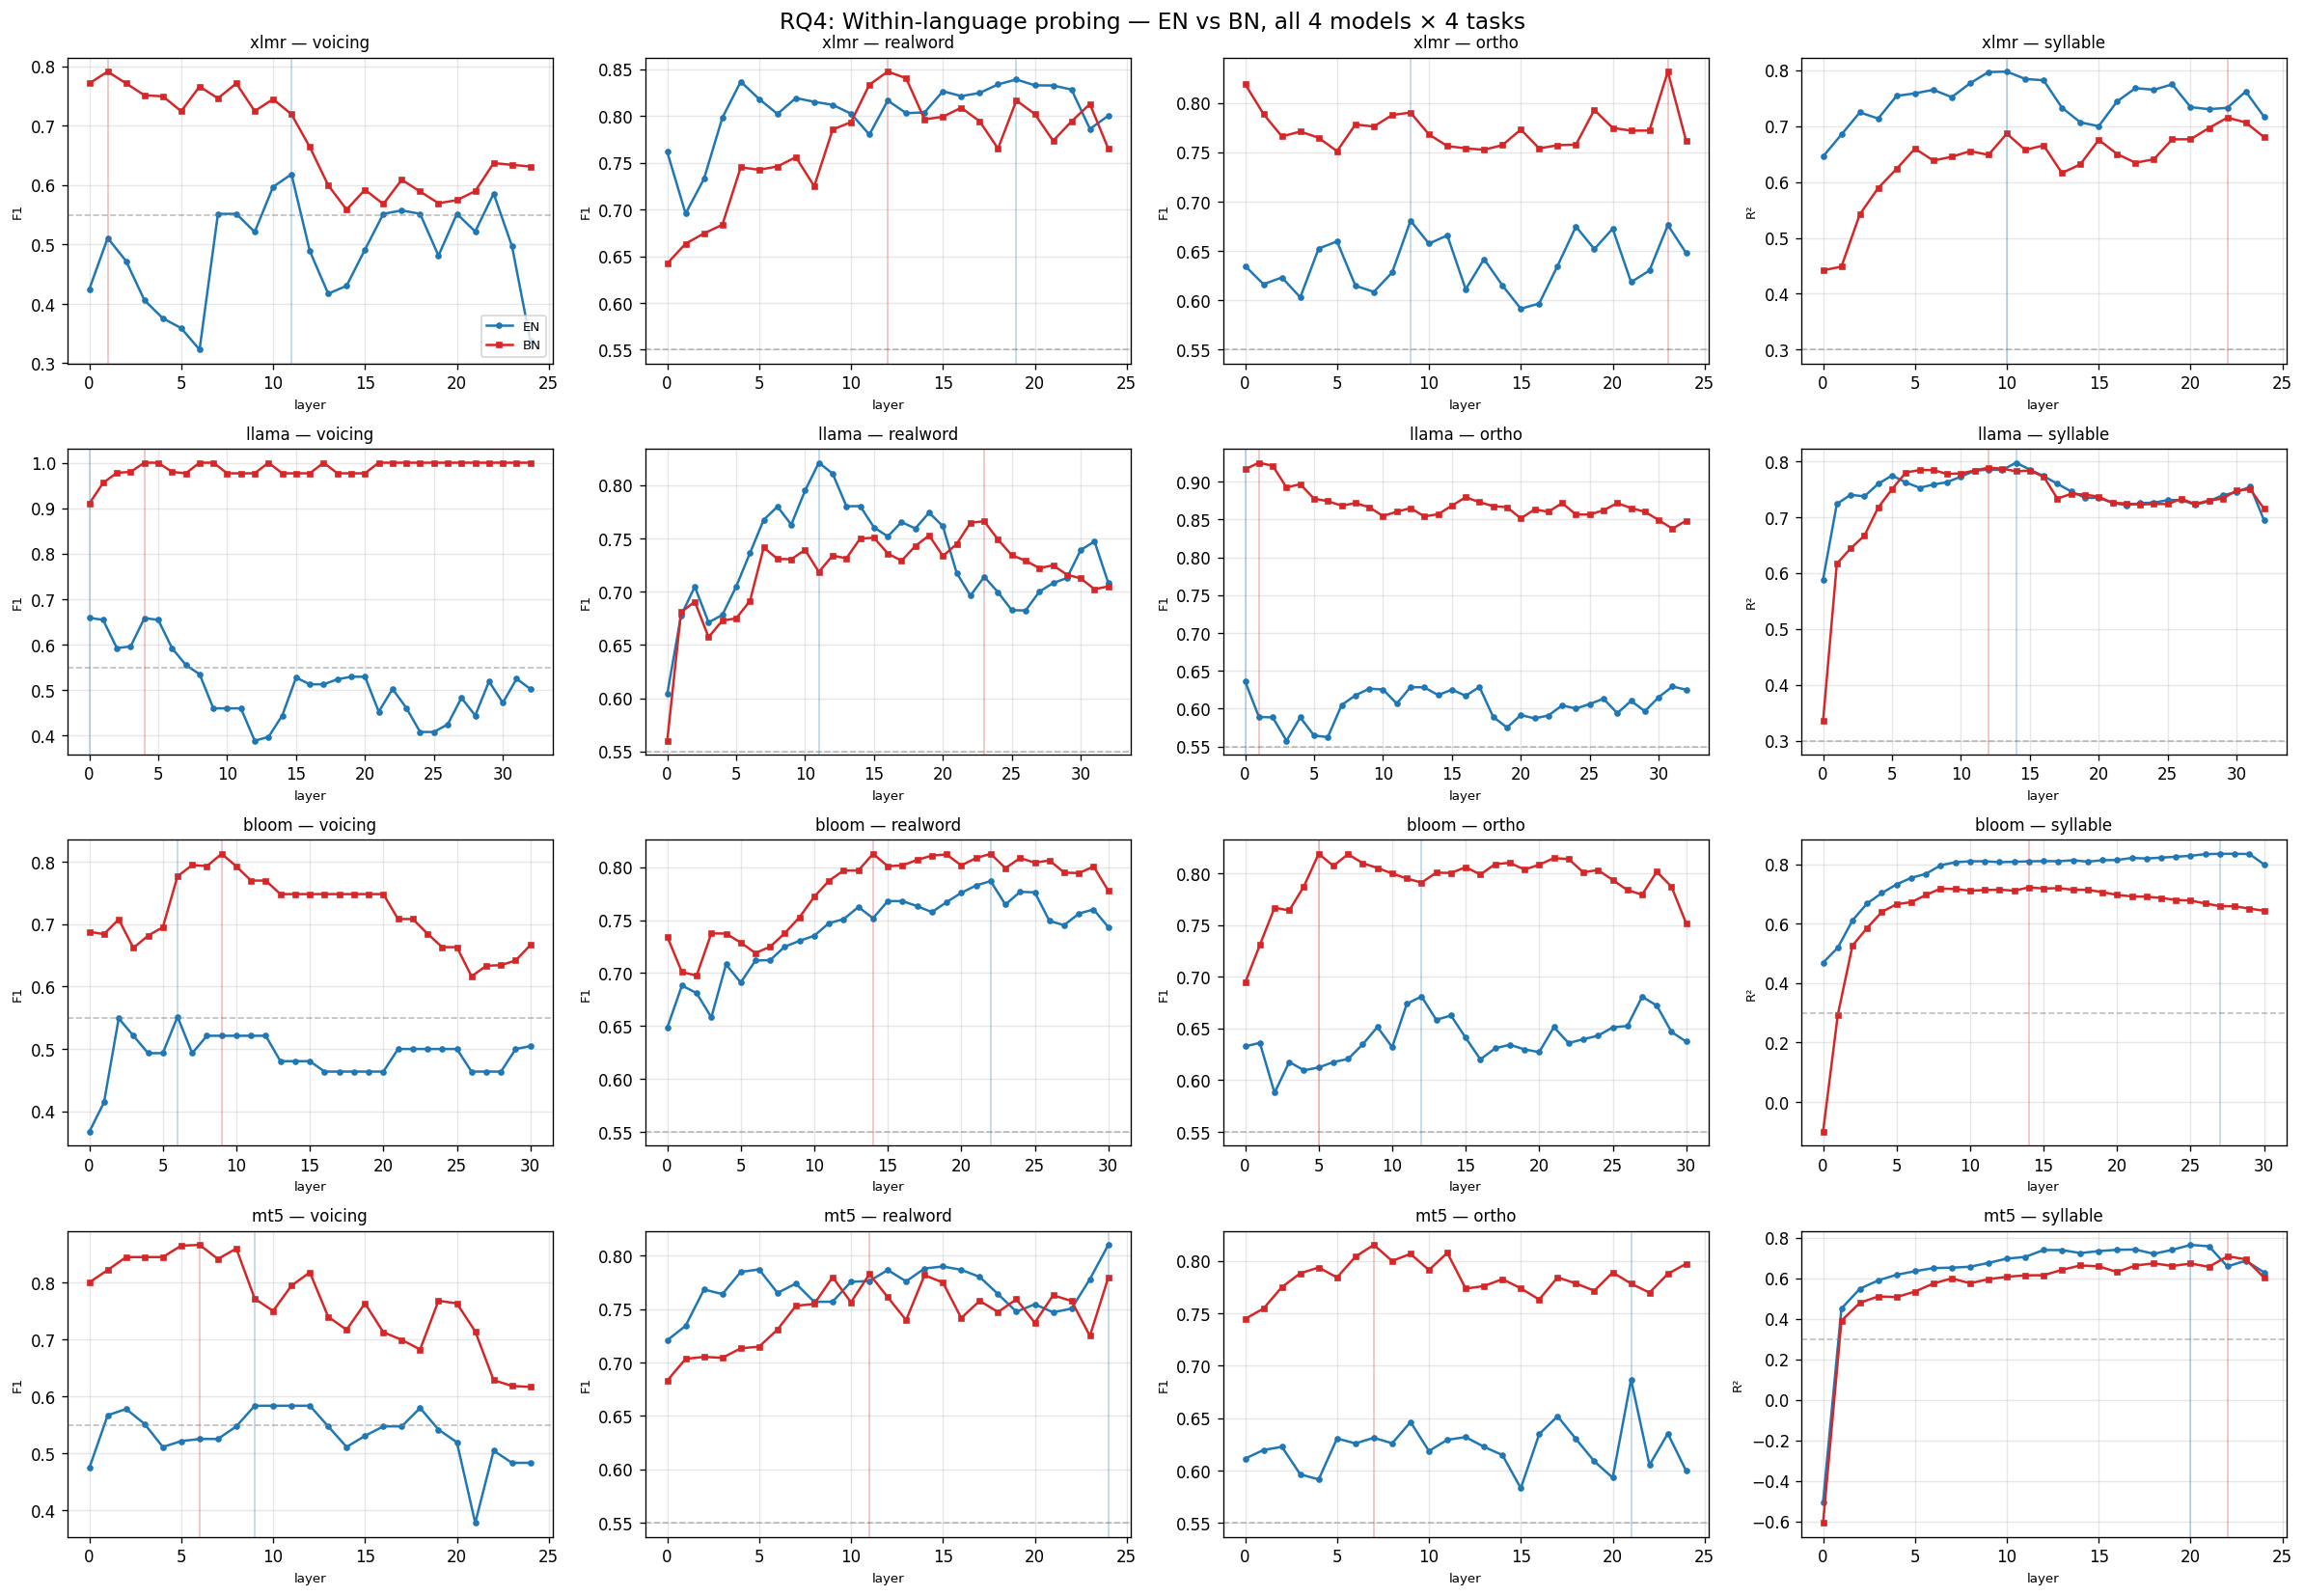
\includegraphics[width=0.95\textwidth]{plots_layer_emergence_all_models.png}
\caption{Layer-emergence trajectories across all four models on the four probing tasks. Subplots align across rows by task; the layer axis is normalised to relative encoder depth.}
\label{fig:layer-emergence}
\end{figure}

\subsection{Surface-feature sanity checks invalidate three of four tasks}
\label{sec:sanity}

The apparent scores in Table~\ref{tab:rq1-en} are striking. Before they are read as phonological evidence, three sanity-check baselines are applied (full methodology in Chapter~4 \S{Surface-feature sanity checks}). The first reads the voicing label off the first character of the word; the second tests whether a five-feature character-statistic baseline beats the LLM probes on orthographic transparency and syllable count; the third matches real and pseudo words on character length within each language and re-probes.

\subsubsection{Voicing: Bangla labels are recoverable from the first character alone}

A leave-one-out probe trained on the layer-0 token-embedding state with a one-hot encoding of the first character recovers Bangla voicing labels with F1 between 0.78 and 0.94 across the four models (Table~\ref{tab:sanity-voicing}); the deterministic upper bound, a rule that reads the first character and assigns voicing, is 1.00. In other words, 100\% of Bangla voicing labels in the stimulus set are inferable from the first character. The probe is therefore reading token identity, not phonological voicing. All Bangla voicing numbers reported in Table~\ref{tab:rq1-en} for RQ1, and any cross-lingual or causal-ablation number subsequently derived from them, reflect first-character recognition rather than a phonological feature.

\begin{table}[H]
\centering
\caption{First-character lookup sanity check (Bangla voicing). LOO F1 at layer~0 versus peak across layers, and deterministic upper bound. All numbers indicate that the voicing label is encoded by the first character of the word.}
\label{tab:sanity-voicing}
\small
\resizebox{\textwidth}{!}{%
\setlength{\tabcolsep}{10pt}
\renewcommand{\arraystretch}{2}
\begin{tabular}{|c|c|c|c|}
\hline
\textbf{Model} & \textbf{L0 LOO F1} & \textbf{Peak LOO F1} & \textbf{Deterministic upper bound} \\
\hline
XLM-R  & 0.80 & 0.83          & 1.00 \\
\hline
Llama  & 0.94 & 1.00 (L2+)    & 1.00 \\
\hline
BLOOM  & 0.78 & 0.80          & 1.00 \\
\hline
mT5    & 0.80 & 0.87          & 1.00 \\
\hline
\end{tabular}%
}
\end{table}

\begin{figure}[H]
\centering
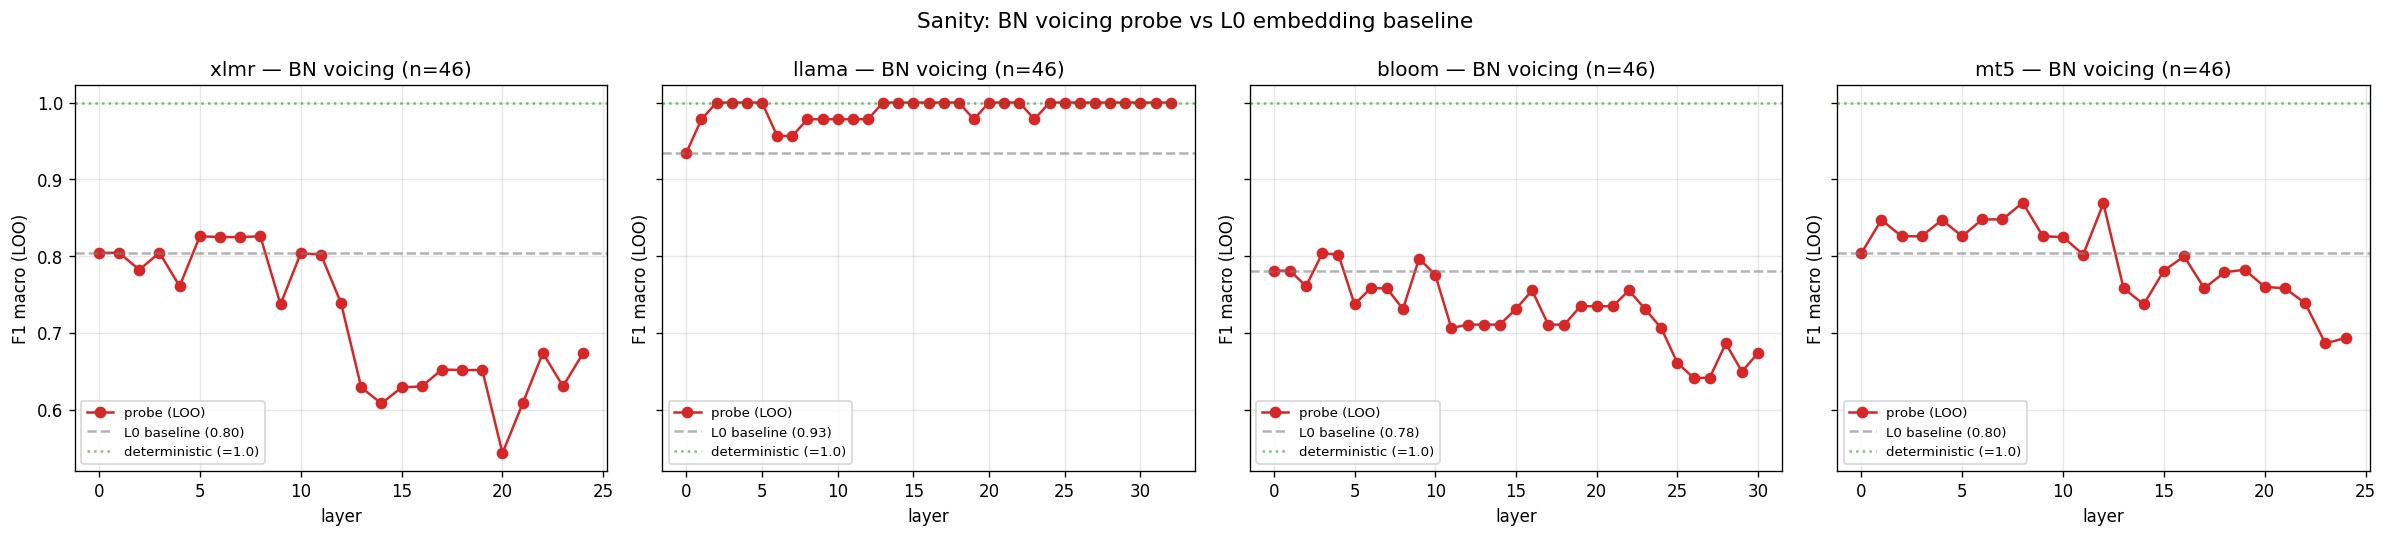
\includegraphics[width=0.85\textwidth]{plots_bn_voicing_sanity.png}
\caption{Bangla voicing sanity check: per-layer leave-one-out probe trained on layer-0 token embeddings recovers voicing labels at F1 0.78--0.94, indicating the labels are inferable from first-character identity alone. The probe is not reading phonological voicing.}
\label{fig:bn-voicing-sanity}
\end{figure}

\subsubsection{Orthographic transparency: solved by character length}

A five-feature surface baseline (character length, byte length, unique-character count, vowel ratio, longest consonant run) reaches F1 0.66 in English and 0.82 in Bangla on the orthographic-transparency task. The best LLM probes gain $\leq +0.03$ in English and $\leq +0.01$ in Bangla over this baseline. The LLM representations do not contribute information above a five-feature character-statistic baseline on this task; the orthographic-transparency task as posed in the stimulus set is a surface task.

\subsubsection{Syllable count: surface-confounded}

The same five-feature baseline reaches $R^2 = 0.81$ on English syllable count and $R^2 = 0.67$ on Bangla. Three of the four LLMs (Llama, mT5, XLM-R) \emph{under-perform} the surface baseline in English; only BLOOM gains $+0.02$. The syllable-count task is also surface-driven.

\subsubsection{Real vs.\ pseudo word: survives length matching}

When real and pseudo words are matched 1:1 on character length (50 matched per language; mean character length 6.88 in English, 5.20 in Bangla), all four models gain at least $+0.20$ F1 over both their layer-0 and the five-feature surface baseline on Bangla (Table~\ref{tab:realword-matched}). The real-versus-pseudo word task is the only one of the four that passes the surface-feature controls and is the only task on which the remainder of this chapter reports cross-lingual transfer, RSA and causal-ablation numbers.

\begin{table}[H]
\centering
\caption{Length-matched realword probing per language. EN/BN at layer 0 versus peak layer, with gain over L0. All four models gain $\geq +0.20$ F1 on Bangla; this is the only task that passes surface-feature controls.}
\label{tab:realword-matched}
\small
\resizebox{\textwidth}{!}{%
\setlength{\tabcolsep}{10pt}
\renewcommand{\arraystretch}{2}
\begin{tabular}{|c|c|c|c|c|c|c|}
\hline
\textbf{Model} & \textbf{EN L0} & \textbf{EN peak} & \textbf{EN gain} & \textbf{BN L0} & \textbf{BN peak} & \textbf{BN gain} \\
\hline
XLM-R & 0.81 & 0.88 & +0.06 & 0.66 & \textbf{0.92} & \textbf{+0.25} \\
\hline
Llama & 0.75 & 0.96 & +0.21 & 0.64 & \textbf{0.90} & \textbf{+0.26} \\
\hline
BLOOM & 0.81 & 0.94 & +0.13 & 0.64 & \textbf{0.94} & \textbf{+0.30} \\
\hline
mT5   & 0.65 & 0.90 & +0.23 & 0.72 & \textbf{0.92} & \textbf{+0.20} \\
\hline
\end{tabular}%
}
\end{table}

\subsection{RQ2: Length-matched cross-lingual transfer}
\label{sec:rq2}

The English-trained length-matched realword probe is evaluated zero-shot on the Bangla length-matched subset. Table~\ref{tab:transfer-matched} reports the surface-controlled cross-lingual numbers; Figures~\ref{fig:four-transfer} and \ref{fig:transfer-matched} visualise the per-layer trajectories and the headline surface-controlled comparison respectively.

\begin{table}[H]
\centering
\caption{Length-matched cross-lingual transfer (EN $\rightarrow$ BN). Peak layer / peak BN F1 / gain over surface baseline / verdict. After surface controls only XLM-R and BLOOM transfer; Llama and mT5 collapse.}
\label{tab:transfer-matched}
\small
\resizebox{\textwidth}{!}{%
\setlength{\tabcolsep}{10pt}
\renewcommand{\arraystretch}{2}
\begin{tabular}{|c|c|c|c|c|}
\hline
\textbf{Model} & \textbf{Peak L (rel.)} & \textbf{Peak BN F1} & \textbf{Gain over surface} & \textbf{Verdict} \\
\hline
XLM-R & L16 / rel.\ 0.67 & \textbf{0.86} & \textbf{+0.24} & real transfer \\
\hline
BLOOM & L25 / rel.\ 0.83 & \textbf{0.92} & \textbf{+0.30} & real transfer \\
\hline
Llama & L31 / rel.\ 0.97 & 0.63          & +0.01           & collapsed to surface \\
\hline
mT5   & L20 / rel.\ 0.83 & 0.60          & $-0.02$         & collapsed below surface \\
\hline
\end{tabular}%
}
\end{table}

\begin{figure}[H]
\centering
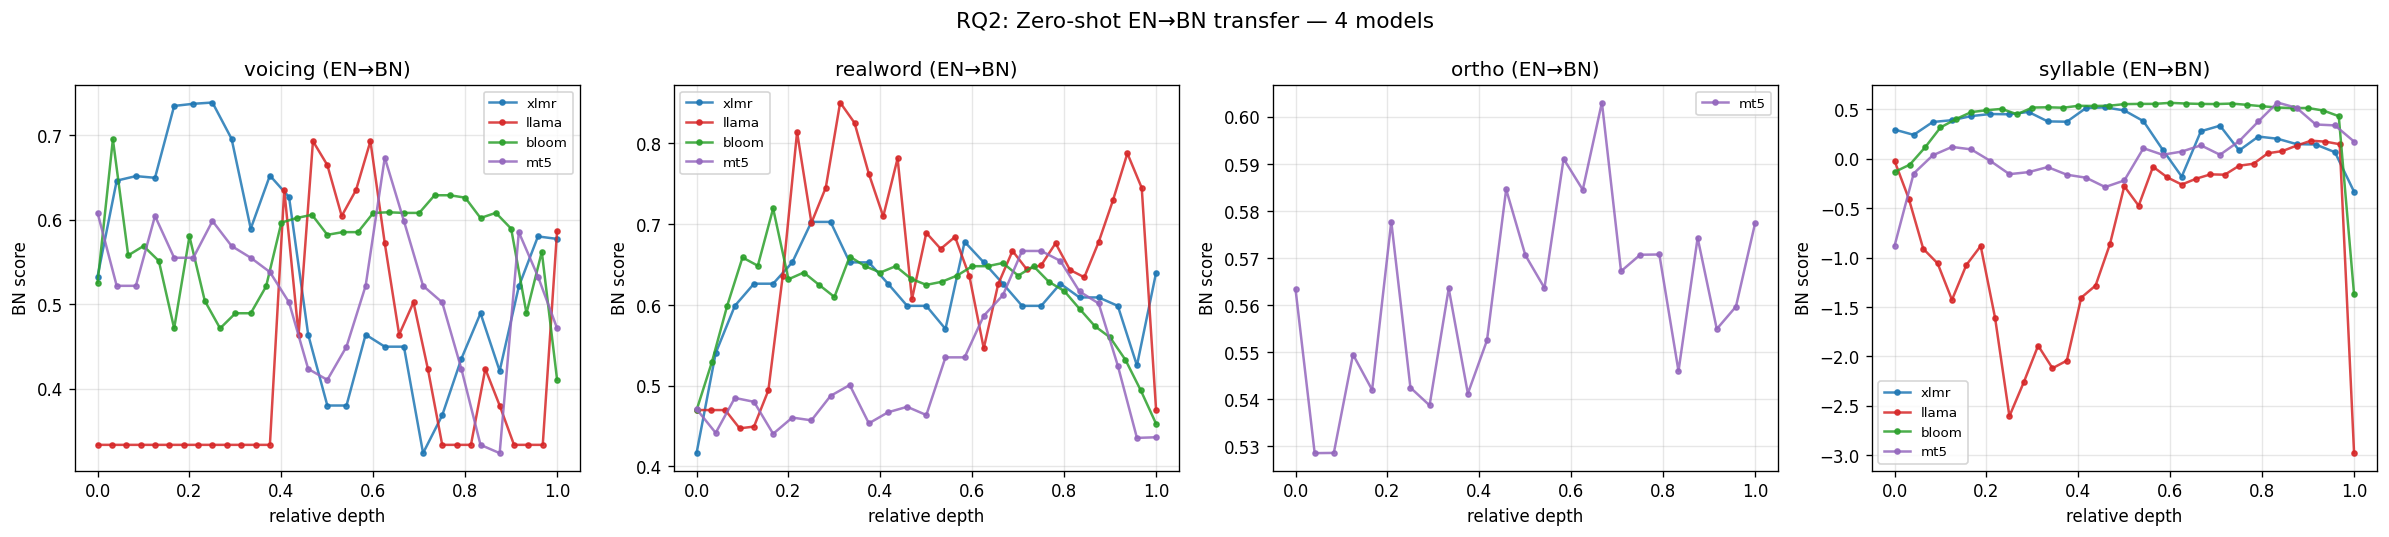
\includegraphics[width=0.95\textwidth]{plots_four_models_transfer.png}
\caption{Per-layer cross-lingual transfer (EN $\rightarrow$ BN) across the four models on all four tasks. Voicing, ortho and syllable curves reflect surface confounds (Section~\ref{sec:sanity}); only the realword curve, length-matched, is interpretable.}
\label{fig:four-transfer}
\end{figure}

\begin{figure}[H]
\centering
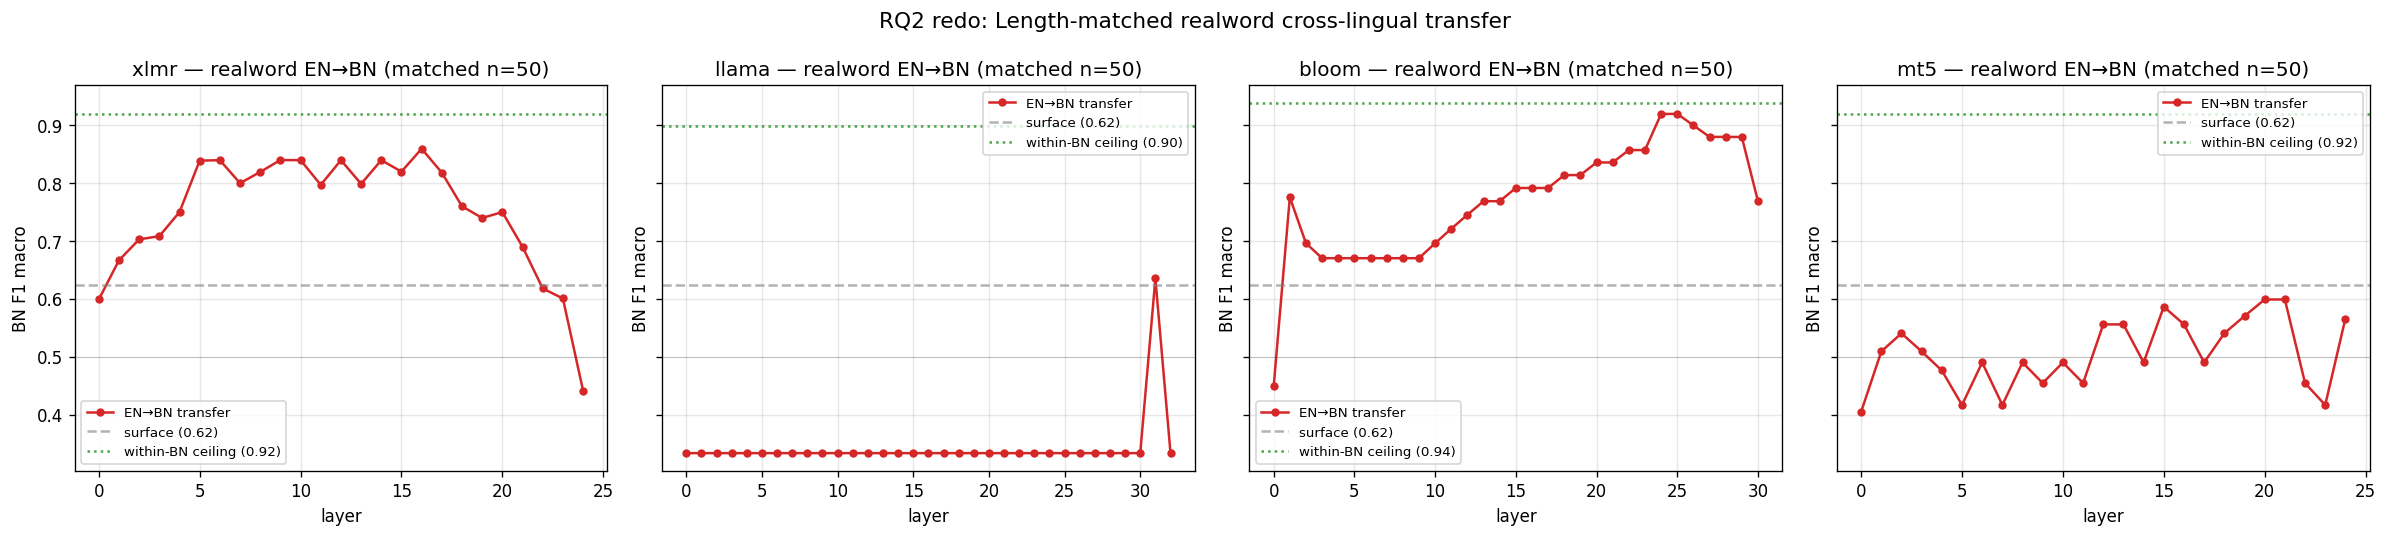
\includegraphics[width=0.95\textwidth]{plots_transfer_realword_matched.png}
\caption{Surface-controlled length-matched real vs.\ pseudo word cross-lingual transfer. XLM-R and BLOOM achieve genuine transfer ($+0.24$ and $+0.30$ over surface respectively); Llama and mT5 collapse to surface level.}
\label{fig:transfer-matched}
\end{figure}

After surface controls only the multilingual masked encoder (XLM-R) and the multilingual causal decoder (BLOOM) achieve genuine cross-lingual real-versus-pseudo word transfer; the English-causal decoder (Llama) and the multilingual span-corruption encoder-decoder (mT5) collapse to surface-baseline level. Two implications follow.

First, pretraining objective and language coverage \emph{jointly} determine cross-lingual transfer. BLOOM beats Llama at similar parameter scale because BLOOM has explicit Bangla coverage in its pretraining mix; XLM-R beats Llama at roughly $13\times$ smaller parameter count because XLM-R is a multilingual MLM encoder. Architecture family alone (encoder-only vs.\ decoder-only) is not predictive: both XLM-R and BLOOM transfer, with very different architectures. Coverage alone (multilingual vs.\ English-heavy) is also not sufficient: mT5 is multilingual and yet collapses; its span-corruption objective appears not to surface cross-lingual lexical similarity at the probe-readable level.

Second, in-language English performance is not a reliable predictor of cross-lingual transfer. Llama reaches the highest in-language English realword F1 (0.96) and the lowest cross-lingual Bangla F1 (0.63); the gap is fully explained by pretraining language coverage. Selecting a model substrate for low-resource Bangla on the basis of English benchmark numbers alone would have picked the worst-transferring model in this comparison.

\subsection{Representational Similarity Analysis corroborates the transfer split}
\label{sec:rsa}

Probing measures whether a feature is linearly recoverable from a representation; Representational Similarity Analysis (RSA) tests whether the geometry of stimulus representations is preserved across languages, independent of any downstream probe. The two methods give consistent answers.

Cross-lingual Representational Dissimilarity Matrix (RDM) Spearman $\rho$ and English $\rightarrow$ Bangla mate-retrieval Top-1 accuracy peak at mid layers for the two transferring models. XLM-R reaches its highest cross-lingual RDM correlation in its middle encoder layers (Figure~\ref{fig:rsa-xlmr}), coincident with the layer at which the length-matched realword probe transfers (L16 in Table~\ref{tab:transfer-matched}). BLOOM reaches Top-1 $0.65$ at L4. Llama reaches Top-1 $0.85$ at L6 in the \emph{unmatched} RSA setting, but this is driven by the same surface confound that inflates its unmatched probing numbers and is reframed by the length-matched probe collapse (Table~\ref{tab:transfer-matched}). The RSA result therefore corroborates the surface-controlled probing result: representational geometry is preserved cross-lingually in XLM-R and BLOOM but not in mT5.

\begin{figure}[H]
\centering
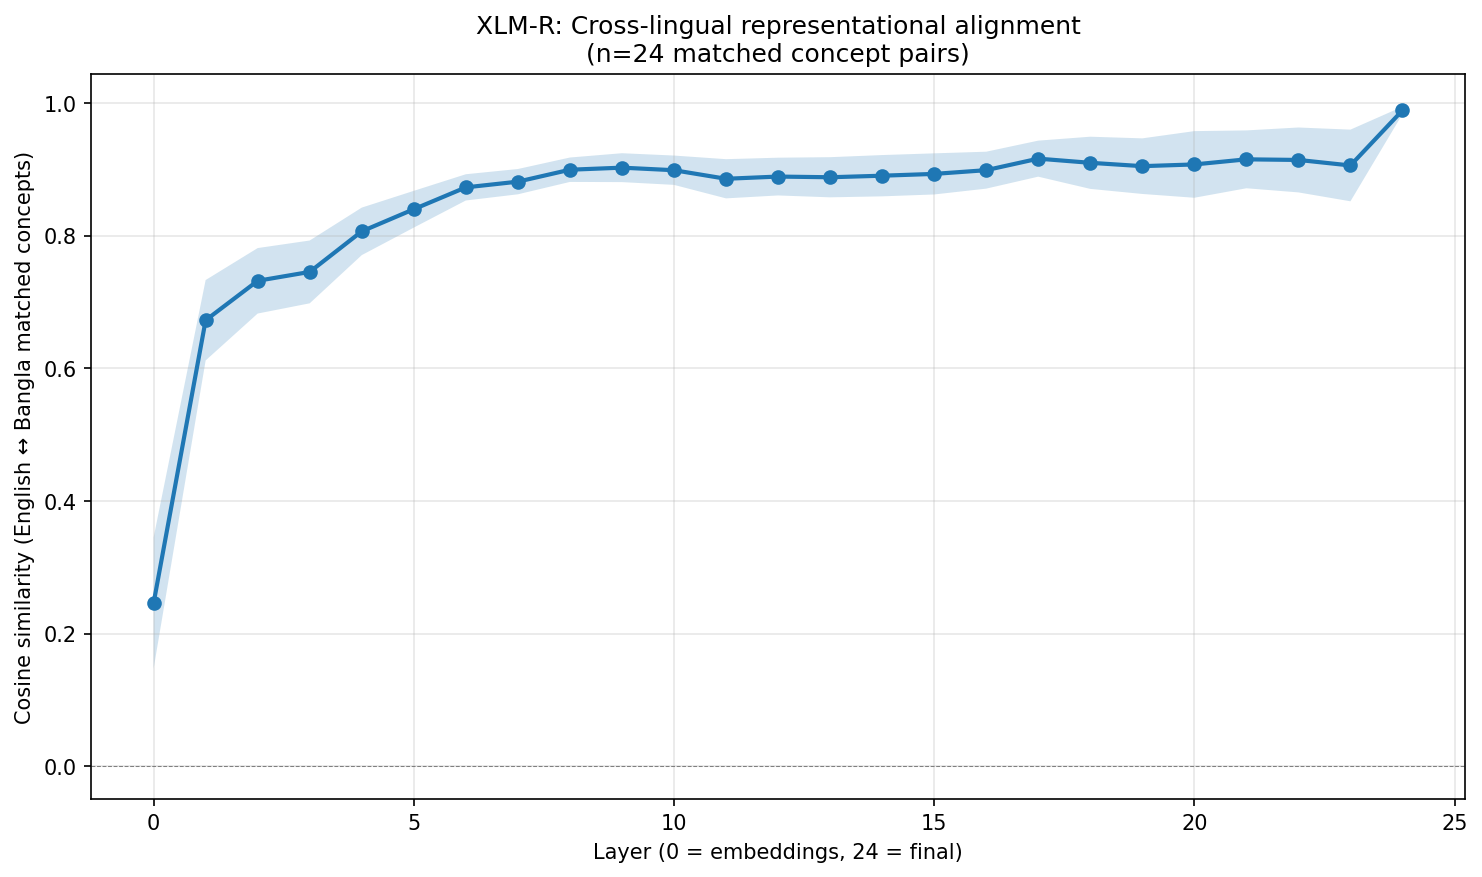
\includegraphics[width=0.75\textwidth]{plots_rsa.png}
\caption{Representational Similarity Analysis for XLM-R: cross-lingual RDM Spearman $\rho$ per layer, with the mate-retrieval Top-1 trajectory overlaid. The mid-encoder peak coincides with the layer at which the length-matched realword probe transfers.}
\label{fig:rsa-xlmr}
\end{figure}

\section{Analysis of Design Solutions}
\label{sec:analysis}

This section addresses RQ3 (mechanism and localisation) by causally testing where each model's cross-lingual lexical signal lives. The analysis combines forward-hook ablation on all four models (Section~\ref{sec:rq3}) with a depth-and-overlap extension on the mT5 encoder (Section~\ref{sec:mt5-localisation}).

\subsection{RQ3: Causal forward-hook ablation on length-matched realword}
\label{sec:rq3}

For each model the length-matched realword probe is first trained on English at the chosen \texttt{measure\_L} layer; ablation hooks three layers earlier zero either the top-20 probe-ranked units or a random-20 control set (averaged over three seeds), and the drop in Bangla F1 is measured. \emph{Ablation specificity} (the top-$K$ drop minus the random-$K$ drop, defined in Chapter~4) is positive when the probe-ranked units carry the causally relevant information, near zero for a distributed encoding, and negative when redundancy is partially undone by ablation.

\begin{table}[H]
\centering
\caption{Causal forward-hook ablation on length-matched realword. mT5 alone shows selective localisation; XLM-R and BLOOM distribute lexical information; Llama has no BN transfer to disrupt.}
\label{tab:ablation-four}
\small
\resizebox{\textwidth}{!}{%
\setlength{\tabcolsep}{10pt}
\renewcommand{\arraystretch}{2}
\begin{tabular}{|c|c|c|c|c|c|}
\hline
\textbf{Model} & \textbf{measure\_L} & \textbf{BN baseline} & \textbf{top20 drop} & \textbf{rand10 drop} & \textbf{specificity} \\
\hline
XLM-R & L8  & 0.78 & $+0.03$    & $+0.02$    & $+0.004$ \\
\hline
Llama & L11 & 0.33 & $0.000$    & $0.000$    & n/a (BN = chance) \\
\hline
BLOOM & L19 & 0.81 & $-0.02$    & $0.00$     & $-0.02$ \\
\hline
\textbf{mT5} & \textbf{L20} & \textbf{0.60} & $\bm{+0.11}$ & \textbf{0.00} & $\bm{+0.11}$ \\
\hline
\end{tabular}%
}
\end{table}

Four observations follow from Table~\ref{tab:ablation-four}.

\textbf{mT5 shows clean specificity.} Zeroing the top-20 probe-ranked units at L17 (three layers below the L20 measure point) drops the Bangla F1 by 0.11, while a random-20 control causes no drop at all. The cross-lingual lexical signal in mT5 is therefore concentrated, not distributed.

\textbf{XLM-R distributes the signal.} Top-20 and random-20 ablation produce essentially the same drop ($+0.03$ vs.\ $+0.02$), so specificity is $+0.004$ (within seed noise). The cross-lingual lexical signal is widely distributed across XLM-R's hidden units; no small subset is causally privileged.

\textbf{BLOOM is also distributed, with mild redundancy.} Specificity is marginally negative ($-0.02$): zeroing the top-20 probe-ranked units slightly \emph{improves} Bangla transfer. This is consistent with distributed redundancy, where multiple unit groups carry overlapping copies of the signal and zeroing one group lets the others dominate. The finding is reported honestly rather than masked.

\textbf{Llama has no BN transfer to disrupt.} Llama's length-matched Bangla baseline is at chance (0.33 F1 with chance $\approx 0.50$ for two-class macro F1; the model's English-trained probe assigns essentially no useful weight to Bangla representations), so ablation can neither improve nor degrade transfer and specificity is not defined.

\begin{figure}[H]
\centering
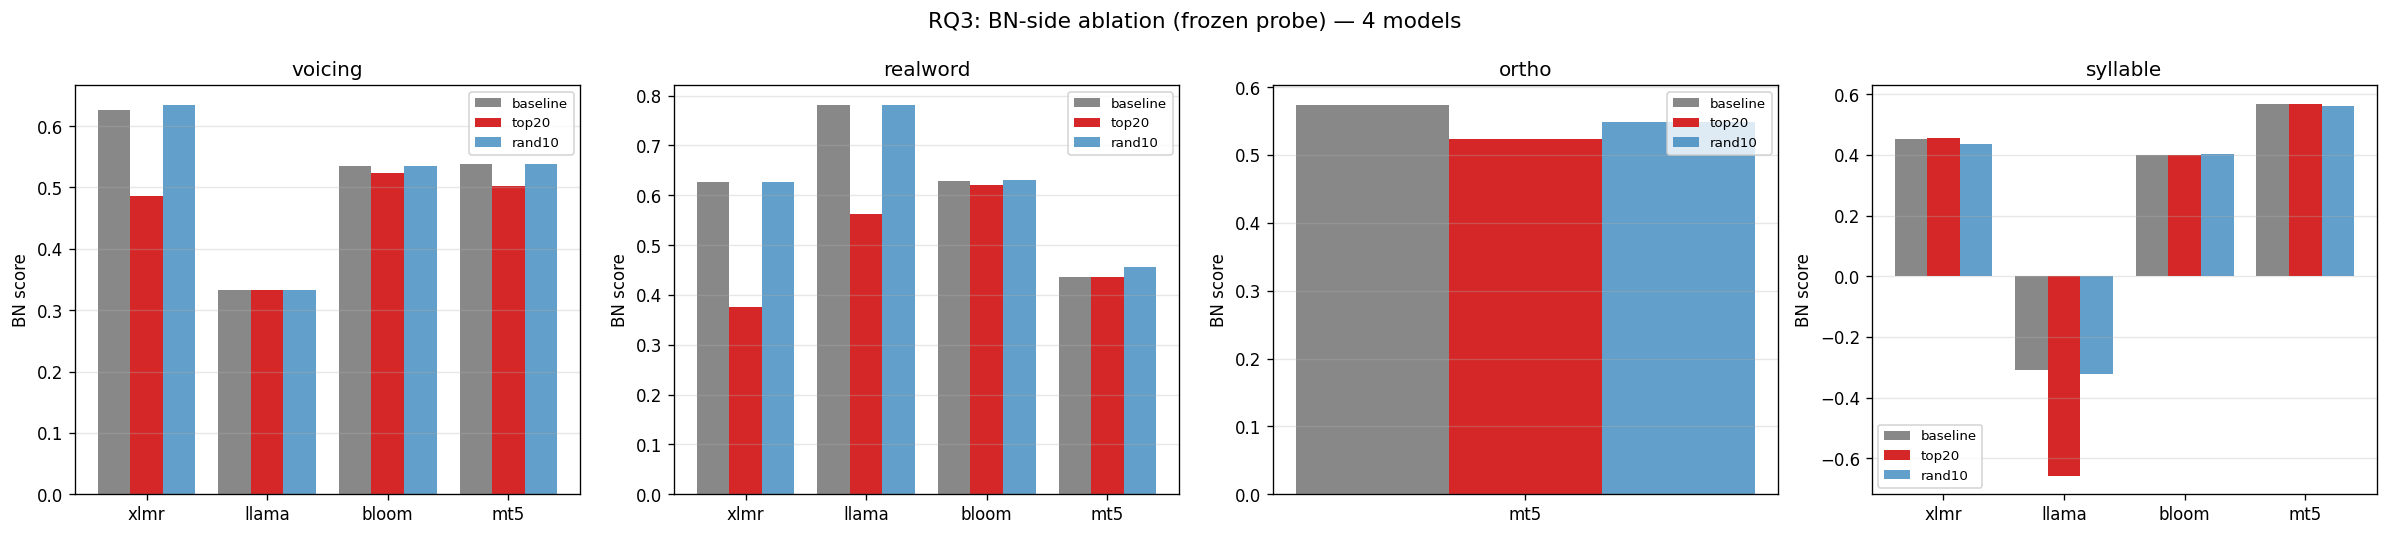
\includegraphics[width=0.95\textwidth]{plots_four_models_ablation.png}
\caption{Four-model causal ablation on length-matched realword. Top-$K$ versus random-$K$ unit ablation on Bangla cross-lingual probe. mT5 shows clean specificity ($+0.11$); XLM-R, BLOOM and Llama do not.}
\label{fig:four-ablation}
\end{figure}

\begin{figure}[H]
\centering
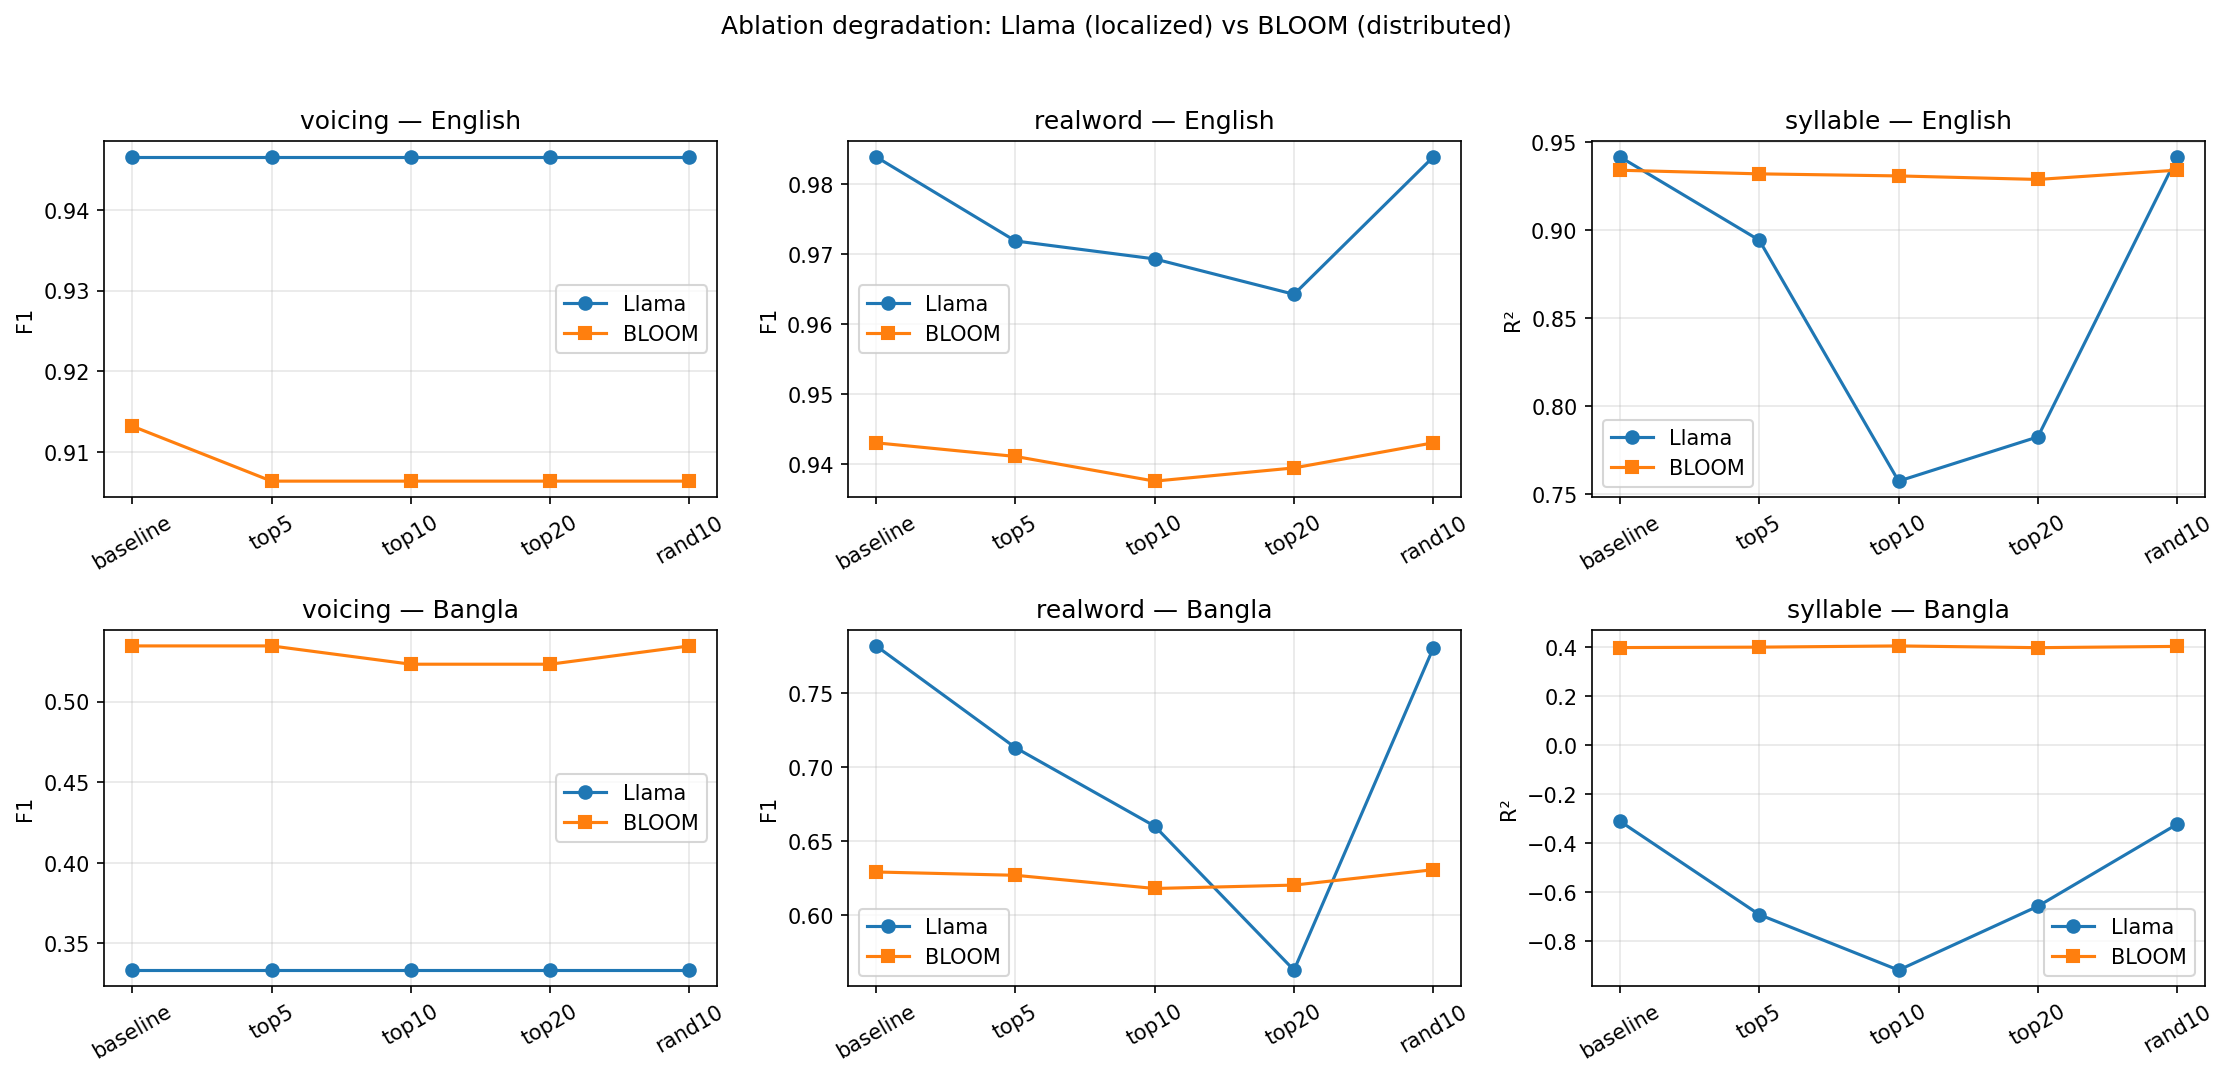
\includegraphics[width=0.85\textwidth]{plots_ablation_llama_vs_bloom.png}
\caption{Llama versus BLOOM ablation degradation curves on length-matched realword. The two decoder-only models diverge: BLOOM's distributed encoding tolerates top-20 ablation; Llama has no Bangla transfer to disrupt in the first place.}
\label{fig:llama-bloom}
\end{figure}

\begin{figure}[H]
\centering
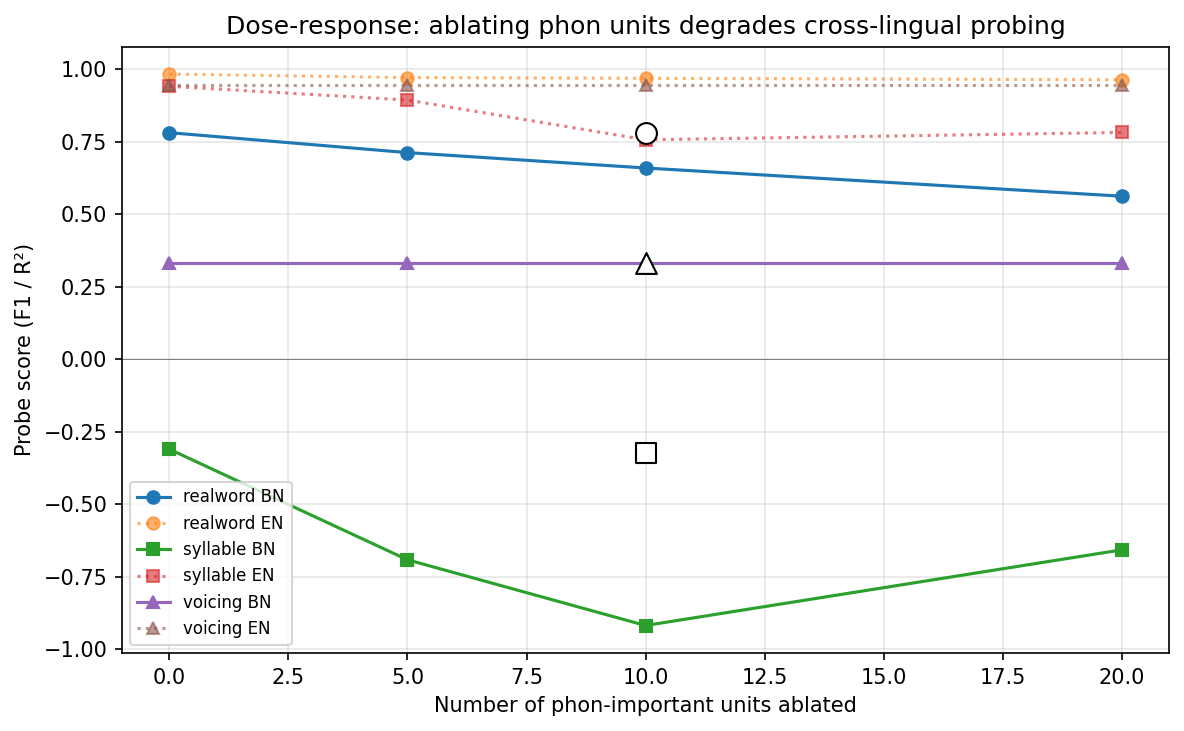
\includegraphics[width=0.85\textwidth]{plots_ablation_doseresponse_llama.png}
\caption{Llama dose-response ablation: BN F1 as a function of the number of zeroed top-ranked units. The curve sits at the chance line, confirming the absence of a localised cross-lingual lexical signal.}
\label{fig:doseresponse-llama}
\end{figure}

\subsection{mT5 localisation across encoder depth (RQ3 extension)}
\label{sec:mt5-localisation}

The L20 ablation showed a $+0.11$ specificity on mT5 (Table~\ref{tab:ablation-four}); a natural follow-up is whether this localisation is a property of the single \texttt{measure\_L} chosen or persists across the encoder. To answer this, the mT5 ablation is repeated at five depths (\texttt{measure\_L} $\in \{4, 8, 12, 16, 20\}$) with three random-unit-control seeds per depth, and the top-10 probe-ranked units at each depth are tracked by Jaccard overlap across depths.

\subsubsection{Localisation persists across encoder depth}

\begin{table}[H]
\centering
\caption{mT5 encoder ablation across depth. Top-10 versus random-mean specificity per measure\_L. Localisation persists across encoder depth; mid-encoder (L12) is strongest.}
\label{tab:mt5-depth}
\small
\resizebox{\textwidth}{!}{%
\setlength{\tabcolsep}{10pt}
\renewcommand{\arraystretch}{2}
\begin{tabular}{|c|c|c|c|c|}
\hline
\textbf{measure\_L} & \textbf{BN baseline} & \textbf{top10 drop} & \textbf{rand mean $\pm$ std} & \textbf{specificity} \\
\hline
L4   & 0.48 & $+0.06$ & $0.00 \pm 0.00$ & $+0.06$ \\
\hline
L8   & 0.49 & $+0.07$ & $0.00 \pm 0.00$ & $+0.07$ \\
\hline
\textbf{L12}  & \textbf{0.56} & $\bm{+0.14}$ & $0.01 \pm 0.01$ & $\bm{+0.13}$ \\
\hline
L16  & 0.56 & $+0.03$ & $-0.01 \pm 0.01$ & $+0.04$ \\
\hline
L20  & 0.60 & $+0.11$ & $0.00 \pm 0.00$ & $+0.11$ \\
\hline
\end{tabular}%
}
\end{table}

Specificity is positive at all five probed depths (range $+0.04$ to $+0.13$); random-unit drops are essentially zero across depths and seeds. mid-encoder L12 shows the strongest effect ($+0.13$), with L8 ($+0.07$) and L20 ($+0.11$) close behind. The result is not a single-layer fluke; it is an architectural property of the mT5 encoder.

\subsubsection{Two persistent backbone units, plus layer-local circuits}

The top-10 probe-ranked units per depth overlap modestly but non-trivially. Chance Jaccard overlap of two size-10 sets drawn from 2048 units is approximately $0.002$; observed pairwise overlaps reach $0.25$ between L4 and L8 and $0.18$ between L8/L12 and L12/L16 (Table~\ref{tab:mt5-overlap}), which is two orders of magnitude above chance.

\begin{table}[H]
\centering
\caption{Top-10 probe-ranked unit Jaccard overlap across mT5 encoder depths. Chance overlap is $\approx 0.002$.}
\label{tab:mt5-overlap}
\small
\resizebox{\textwidth}{!}{%
\setlength{\tabcolsep}{10pt}
\renewcommand{\arraystretch}{2}
\begin{tabular}{|c|c|c|c|c|c|}
\hline
 & \textbf{L4} & \textbf{L8} & \textbf{L12} & \textbf{L16} & \textbf{L20} \\
\hline
\textbf{L4}   & 1.00 & 0.25 & 0.05 & 0.11 & 0.00 \\
\hline
\textbf{L8}   & 0.25 & 1.00 & 0.18 & 0.18 & 0.05 \\
\hline
\textbf{L12}  & 0.05 & 0.18 & 1.00 & 0.18 & 0.05 \\
\hline
\textbf{L16}  & 0.11 & 0.18 & 0.18 & 1.00 & 0.05 \\
\hline
\textbf{L20}  & 0.00 & 0.05 & 0.05 & 0.05 & 1.00 \\
\hline
\end{tabular}%
}
\end{table}

Two units appear in the top-10 at four out of five probed depths: \textbf{u782} (in the top-10 at L4, L8, L12, L16) and \textbf{u1880} (in the top-10 at L8, L12, L16, L20). Of the 38 unique units that appear in any top-10 set across the five depths, 31 are layer-specific (appear at only one depth). The pattern is therefore \emph{hybrid}: a small persistent backbone of two cross-depth units, plus a much larger pool of layer-local specialised circuits, with graceful hand-off between them as depth increases. Neither a purely static channel theory (in which the same units carry the same information at every layer) nor a purely dynamic routing theory (in which each layer uses an entirely fresh set of units) fits the data; the truth is a mixture.

\begin{figure}[H]
\centering
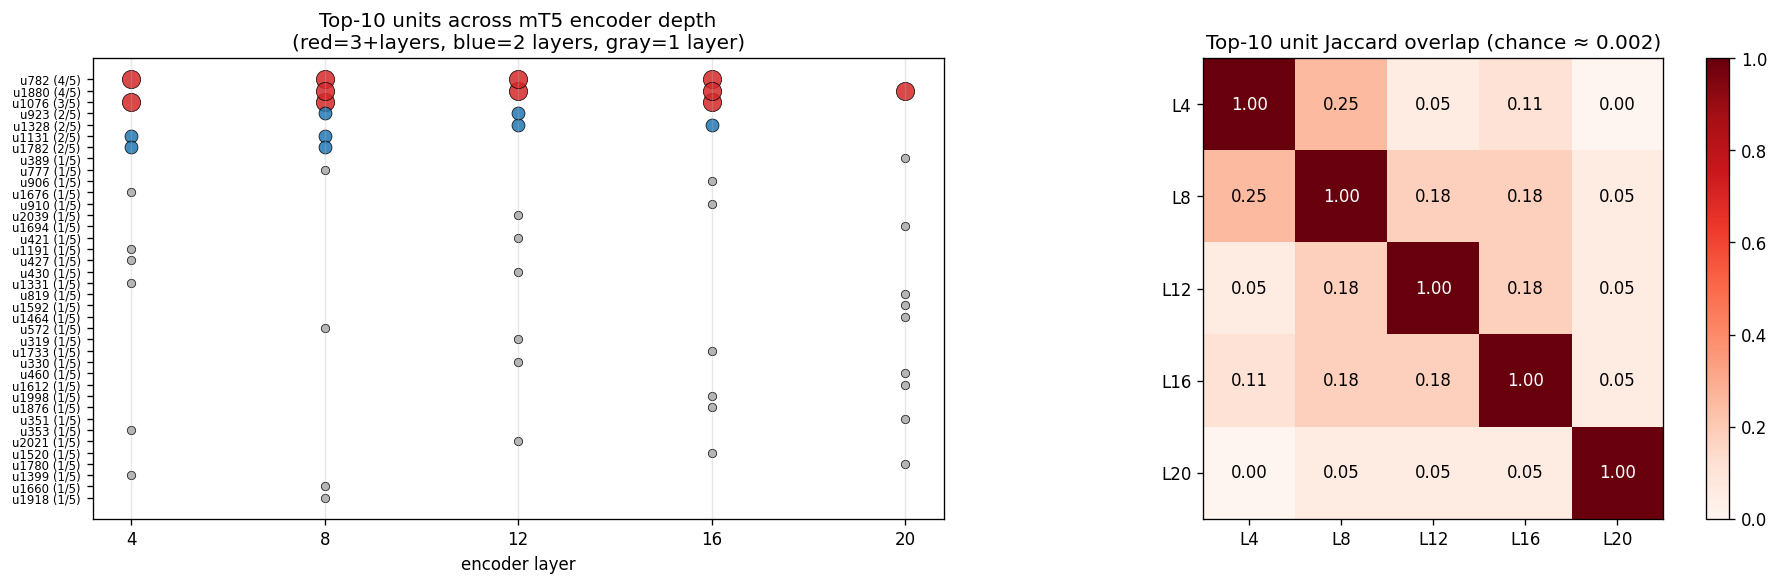
\includegraphics[width=0.85\textwidth]{plots_mt5_unit_overlap.png}
\caption{mT5 top-10 probe-ranked unit overlap (Jaccard) across encoder depths. Two persistent backbone units \{\textbf{u782}, \textbf{u1880}\} recur at $\geq 4$ of the 5 probed depths each; 31 of 38 unique top-10 units are layer-specific.}
\label{fig:mt5-overlap}
\end{figure}

\section{Final Design Adjustments}
\label{sec:adjustments}

Two design adjustments were made as a direct consequence of the results above.

First, the original RQ1 set of four phonological tasks (voicing, realword, ortho, syllable) was reduced to one (length-matched realword) for all RQ2 and RQ3 reporting, on the basis of Section~\ref{sec:sanity}. The original tables for the other three tasks are kept in Table~\ref{tab:rq1-en} only as the baseline against which the surface-feature failure is documented. This pruning is the central methodology contribution of the thesis.

Second, the ablation analysis was extended from a single \texttt{measure\_L} to a five-depth scan with three random-unit-control seeds per depth, after the L20 ablation showed a $+0.11$ specificity on mT5 (Table~\ref{tab:ablation-four}). The depth-scan result (Table~\ref{tab:mt5-depth}) and the Jaccard overlap analysis (Table~\ref{tab:mt5-overlap}, Figure~\ref{fig:mt5-overlap}) together establish the two-backbone-units finding (\{u782, u1880\}), which is the central mechanism contribution of the thesis.

\section{Statistical Analysis}
\label{sec:stats}

Probe performance is reported at the peak layer with the cross-validated mean across a 5-fold split of the English training set. Reported numbers are point estimates rather than confidence intervals because the length-matched subsets are small ($n = 50$ per language) and per-fold variance is dominated by stimulus-level idiosyncrasy. Where reported, ablation random-unit controls use three independent random seeds; the standard deviation across seeds is reported in Table~\ref{tab:mt5-depth} (typically $\leq 0.01$).

The persistence of u782 and u1880 across encoder depths is established by exhaustive enumeration of the top-10 probe-ranked units per depth, not by a statistical test. The relevant null is the chance Jaccard overlap of two random size-10 sets drawn from 2048 units, which is approximately $0.002$. The observed pairwise overlaps in Table~\ref{tab:mt5-overlap} range from $0.05$ to $0.25$ for the depth pairs that share at least one backbone unit; even the smallest of these observed values is roughly $25\times$ above chance, and the largest is roughly $125\times$ above chance. The backbone finding is therefore not a chance recurrence.

\section{Comparisons and Relationships}
\label{sec:comparisons}

\subsection{RQ4: Cross-model comparison and model selection}
\label{sec:rq4}

\subsubsection{Five comparative observations}

\begin{enumerate}
    \item \textbf{Best cross-lingual transfer (length-matched BN F1):} BLOOM ($0.92$, $+0.30$ over surface) $>$ XLM-R ($0.86$, $+0.24$) $\gg$ Llama ($0.63$, $+0.01$) $>$ mT5 ($0.60$, $-0.02$).
    \item \textbf{Best parameter efficiency:} XLM-R reaches $0.86$ BN F1 at $0.56$B parameters, roughly $13\times$ smaller than BLOOM ($7.1$B). Multilingual MLM-encoder pretraining is highly parameter-efficient for cross-lingual lexical structure.
    \item \textbf{Best in-language English realword:} Llama ($0.96$) $>$ BLOOM ($0.94$). English-causal pretraining dominates in English; the gap reverses cross-lingually.
    \item \textbf{Best causal localisation:} mT5 alone shows clean ablation specificity ($+0.11$ at L20, $+0.13$ at L12), with two persistent backbone units (u782, u1880) spanning the encoder. No other model in the comparison localises the cross-lingual lexical signal.
    \item \textbf{Pretraining objective and coverage dominate scale.} A $0.56$B multilingual encoder (XLM-R) beats an $8$B English-heavy decoder (Llama) on cross-lingual transfer; depth and width do not compensate for pretraining-language gaps.
\end{enumerate}

\subsubsection{Model-selection: paired recommendation}

The four models are not interchangeable; each dominates a different criterion. The thesis therefore issues a \emph{paired} recommendation rather than a single best-model claim:

\begin{itemize}
    \item \textbf{For a practical low-resource Bangla screening prototype:} BLOOM 7B1. Highest cross-lingual transfer ($0.92$ Bangla F1), survives surface controls, can be deployed as a frozen feature extractor without fine-tuning.
    \item \textbf{For interpretability and mechanism studies:} mT5 XL. The only model in the comparison whose cross-lingual lexical signal localises to a small unit set with a persistent two-unit backbone.
    \item \textbf{For hardware-constrained deployments:} XLM-RoBERTa large. At $0.56$B parameters it delivers $0.86$ Bangla F1 and runs in 16-bit on a single consumer GPU.
    \item \textbf{Not recommended:} Llama 3.1 8B for any cross-lingual Bangla setting at the lexical level. Length-matched transfer collapses to $0.63$ Bangla F1 (gain $+0.01$ over surface).
\end{itemize}

\subsection{Relationship to prior work}

The cross-lingual transfer numbers for XLM-R and BLOOM are consistent with the broader multilingual probing literature \cite{conneau2020xlmr,wu2020emerging,pires2019mbert}, but the gain-over-surface numbers we report are smaller than the gain-over-chance numbers commonly reported in earlier work. The difference is fully explained by the first-character lookup baseline and the length-matching control. The mT5 localisation result is new: prior interpretability work on multilingual models reports language-neutral and language-specific neurons in masked encoders \cite{stanczak2022neurons}, but not concentrated cross-lingual lexical coding with persistent backbone units in an encoder-decoder.

\section{Discussion}
\label{sec:discussion}

\subsection{Interpretation}

The headline finding is the joint role of pretraining objective and pretraining language coverage. The two transferring models (XLM-R and BLOOM) both have explicit Bangla coverage in their pretraining mix; the two collapsing models do not, in two different ways. Llama lacks Bangla coverage entirely; mT5 has multilingual coverage but its span-corruption objective does not surface cross-lingual lexical similarity at the probe-readable level on the length-matched task. BLOOM's multilingual causal-LM pretraining produces \emph{distributed} lexical representations that transfer well in raw performance but resist localisation; mT5's span-corruption encoder-decoder pretraining produces \emph{concentrated} lexical representations that survive at the unit level but do not surface in the length-matched cross-lingual probe at high F1. The two models are therefore complementary along the practical-vs-interpretable axis: BLOOM is the practical substrate, mT5 is the interpretability substrate.

The mT5 backbone-plus-routing pattern established in Section~\ref{sec:mt5-localisation} is itself a non-trivial mechanism finding. The hybrid organisation -- two persistent backbone units coexisting with a larger pool of layer-local circuits -- suggests a graceful hand-off architecture inside the mT5 encoder that, to our knowledge, has not been previously documented for multilingual lexical content.

\subsection{Implications}

For practitioners, the implications follow directly from the paired recommendation of Section~\ref{sec:rq4} and are not re-enumerated here: the substrate should be chosen against the deployment goal -- raw cross-lingual transfer, interpretability, or parameter efficiency -- because no single model dominates all three axes.

For the probing literature, the implication is methodological: the first-character lookup baseline (or its equivalent in the target language) and the length-matching control should be standard preconditions for any phonological probing claim. Three of four standard tasks in our setting fail these controls, and the cross-lingual signal reported in prior work likely reflects character statistics or token identity to a greater extent than usually acknowledged.

\subsection{Limitations}
\label{sec:caveats}

Five limitations bound the interpretation.

\begin{itemize}
    \item Bangla voicing labels in the original stimulus set are recoverable from the first character; the original \texttt{voiced\_unvoiced} column for Bangla is unusable for phonological probing as posed, and all Bangla voicing numbers in the original RQ1--RQ3 tables reflect first-character recognition.
    \item Length-matched subsets are small ($n = 50$ per language). Per-layer scores have meaningful variance; the gain-over-surface numbers are point estimates.
    \item The frozen probe English baseline reaches $1.00$ after matching; only the Bangla drop is interpretable as a causal signal in the ablation.
    \item Architectural confound: mT5 is the only encoder-decoder probed. The mT5 localisation result could reflect the span-corruption objective, the encoder-decoder split, or both; resolving this would require probing additional encoder-decoder models (e.g.\ ByT5, T5).
    \item BLOOM's ablation specificity is marginally negative ($-0.02$): zeroing the top-20 probe-ranked units \emph{slightly improves} Bangla transfer, which is consistent with distributed redundancy rather than a clean null. This is reported honestly rather than masked.
\end{itemize}


\chapter{Conclusion}
\section{Summary of Findings}

This thesis probed four publicly released multilingual large language models -- XLM-RoBERTa large, Llama 3.1 8B, BLOOM 7B1 and mT5 XL -- for cross-lingual lexical and phonological structure using a curated 440-stimulus English / Bangla dataset, per-layer linear probes, surface-feature sanity controls, Representational Similarity Analysis and causal forward-hook ablation. Five headline findings emerged.

First, three of four standard phonological probing tasks (voicing, orthographic transparency, syllable count) fail surface-feature sanity checks. Bangla voicing labels in the original stimulus set are recoverable from the first character of each word with $\geq 0.78$ F1 across all four models; orthographic and syllable probes do not improve over a five-feature character-statistic baseline. Apparent cross-lingual phonological encoding in prior work likely reflects character statistics or token identity rather than phonological structure.

Second, the surviving task -- length-matched real-versus-pseudo word discrimination -- shows genuine cross-lingual transfer in two of the four models. BLOOM 7B1 reaches $0.92$ Bangla F1 ($+0.30$ over surface) and XLM-RoBERTa large reaches $0.86$ ($+0.24$ over surface). Llama 3.1 8B collapses to $0.63$ ($+0.01$) and mT5 XL collapses to $0.60$ ($-0.02$).

Third, the determinant of transfer is the joint effect of pretraining objective and pretraining language coverage. The $0.56$B multilingual MLM-encoder (XLM-R) beats the $8$B English-heavy causal decoder (Llama) by more than two F1 points; depth and width do not compensate for pretraining-language gaps.

Fourth, mT5 alone exhibits concentrated cross-lingual lexical coding. Causal forward-hook ablation across five encoder depths shows clean specificity ($+0.04$ to $+0.13$); two persistent backbone units (u782 and u1880) appear in the top-10 probe-ranked units at four out of five probed depths each. The mT5 mechanism is hybrid: a small persistent backbone plus layer-local specialised circuits.

Fifth, the four models are not interchangeable. BLOOM is the practical substrate for raw cross-lingual transfer; mT5 is the interpretability substrate for mechanism studies; XLM-R is the parameter-efficient substrate for hardware-constrained deployments; Llama is not recommended for any cross-lingual Bangla setting at the lexical level.

\section{Contributions to the Field}

This thesis makes four contributions.

\textbf{Methodological.} Surface-feature sanity checks (first-character lookup baseline; five-feature character-statistic baseline; 1:1 length matching) are shown to invalidate three of four standard phonological probing tasks. The check protocol generalises and is proposed as a minimum standard for any future probing of multilingual LLMs at the lexical / sub-lexical level.

\textbf{Empirical.} The first surface-controlled, four-architecture, two-language (English / Bangla) probing study at the lexical level. Per-task, per-model, per-layer numbers are reported in CSV form alongside their plots, and the headline four-model and three-model comparison tables are committed to the public repository.

\textbf{Mechanistic.} The mT5 cross-lingual lexical signal is localised to approximately ten encoder units; two units (u782, u1880) persist as a backbone across more than half of the probed encoder depths. To our knowledge, this is the first demonstration of concentrated cross-lingual lexical coding with a persistent unit backbone in a multilingual encoder-decoder.

\textbf{Translational.} A model-selection recommendation grounded in surface-controlled performance, parameter efficiency and interpretability is issued: BLOOM 7B1 for practical low-resource Bangla screening prototypes, mT5 XL for interpretability, XLM-R for parameter-efficient deployments. The recommendation is bounded explicitly to ``substrate for downstream supervised prototypes'' and not to ``diagnostic tool.''

\section{Recommendations for Future Work}

Six concrete directions follow from these results.

\begin{enumerate}
    \item \textbf{Native-clinician supervision.} Before any of the recommended substrates is used on children, a supervised clinical pipeline must be built: stimulus selection by Bangla speech-and-language clinicians, validation against an existing diagnostic battery and longitudinal follow-up. The probing results in this thesis are a precondition, not a substitute, for that pipeline.

    \item \textbf{Stimulus expansion.} The length-matched real-versus-pseudo word subset is $n = 50$ per language. Expanding to $n \geq 500$ matched pairs per language, with stratification by syllable count and morphological complexity, would reduce per-layer variance and support stronger ablation-specificity claims.

    \item \textbf{Encoder-decoder confound.} mT5 is the only encoder-decoder probed. Replicating the depth-scan ablation on ByT5, T5 and a multilingual T5-style model trained without span corruption would isolate whether the localisation is driven by the objective, by the encoder-decoder split, or both.

    \item \textbf{Mechanism follow-up on the two backbone units.} What information do u782 and u1880 actually carry? Stimulus-conditional firing analyses, ablation conjunctions (zeroing both units simultaneously versus singly) and sparse-autoencoder projection would localise the linguistic content of the persistent backbone.

    \item \textbf{Language coverage.} The present study covers Bangla. Extending to Hindi, Tamil, Urdu and Swahili (all under-served languages, all in BLOOM's pretraining mix) would test whether the BLOOM transfer recipe generalises across South-Asian and African languages or is specific to Bangla.

    \item \textbf{Clinical-task expansion.} The probing tasks in this thesis cover real-versus-pseudo word discrimination only after sanity checks. Future work should design surface-controlled probes for rapid automatised naming, non-word repetition and rhyme detection, which together constitute the full phonological-processing battery in CTOPP-2 and analogous clinical instruments.
\end{enumerate}

The longer arc is the same: low-resource clinical NLP can ride on frozen multilingual substrates if -- and only if -- the substrates are evaluated honestly. The sanity-check failure of three of four standard tasks reported here is, in that sense, the most useful single finding of the thesis: it tells the next study where the floor is.


% Bibliography is skipped in draft mode (saves the BibTeX pass)
\ifdraftmode\else
\phantomsection
\bibliographystyle{ieeetr}
\bibliography{bibliography/references}
\fi

\newpage
\phantomsection
\addcontentsline{toc}{chapter}{Appendix A: Tools, Software, Hardware and Reproducibility}
\chapter*{Appendix A: Tools, Software, Hardware and Reproducibility}
\addcontentsline{toc}{section}{Software stack}

\section*{Software stack}

\begin{table}[H]
\centering
\small
\renewcommand{\arraystretch}{1.5}
\begin{tabularx}{\textwidth}{|L|L|}
\hline
\textbf{Component} & \textbf{Version} \\
\hline
Python & 3.10 \\
\hline
PyTorch & 2.1+ (CUDA 11.8 / 12.1) \\
\hline
Hugging Face \texttt{transformers} & $\geq$ 4.40 \\
\hline
\texttt{tokenizers} & $\geq$ 0.15 \\
\hline
\texttt{accelerate} & $\geq$ 0.27 \\
\hline
\texttt{bitsandbytes} & $\geq$ 0.43 \\
\hline
\texttt{unsloth} & 2024.x (latest at run) \\
\hline
\texttt{scikit-learn} & 1.3+ \\
\hline
\texttt{numpy} & 1.26+ \\
\hline
\texttt{pandas} & 2.1+ \\
\hline
\texttt{matplotlib} & 3.8+ \\
\hline
\texttt{seaborn} & 0.13+ \\
\hline
\texttt{scipy} & 1.11+ (Spearman, ranking) \\
\hline
\end{tabularx}
\caption{Software dependencies and pinned versions.}
\end{table}

Per-model environment files (\texttt{dys-env}, \texttt{dys-llm-env}, \texttt{dys-env-bloom}, \texttt{dys-mt5-env}) are committed in each model directory and contain exact pinned versions.

\section*{Hardware}

All experiments were executed on a single NVIDIA consumer GPU with 24~GB VRAM. XLM-R large ($0.56$B) and the mT5 XL encoder ($1.67$B) were probed in 16-bit precision. Llama 3.1 8B and BLOOM 7B1 were loaded with 4-bit weight quantisation via Unsloth and bitsandbytes \cite{dettmers2022bnb}; per-layer hidden states were extracted in 16-bit and pooled to a single fixed-dimensional vector per item per layer. Aggregate compute footprint across the four models is under 30 GPU-hours.

\section*{Reproducibility}

\subsection*{Random seeds}

\begin{itemize}
    \item Probe train/test split: \texttt{random\_state=42} (scikit-learn).
    \item 5-fold cross-validation: \texttt{random\_state=42}.
    \item Ablation random-unit controls (mT5 depth scan): seeds \{0, 1, 2\}.
    \item PyTorch CUDA determinism is not enforced because frozen-forward inference is deterministic for the operations used; small numerical drift between hardware generations is expected but does not affect any reported peak-layer choice.
\end{itemize}

\subsection*{Data and result artefacts}

Each per-model directory contains:
\begin{itemize}
    \item \texttt{main.ipynb} -- the end-to-end notebook (representation extraction $\rightarrow$ probing $\rightarrow$ ablation).
    \item \texttt{dyslex\_probe\_stimuli\_clean.csv} -- the 440-stimulus dataset (identical across all four directories).
    \item \texttt{representations/} -- per-layer hidden-state caches (one tensor per layer per language).
    \item \texttt{results\_english\_probing\_*.csv}, \texttt{results\_transfer\_*.csv}, \texttt{results\_rsa\_*.csv}, \texttt{results\_ablation\_*.csv}, \texttt{results\_*\_realword\_matched.csv} -- result tables.
    \item \texttt{plots\_*.png} -- figures.
\end{itemize}

The mT5 directory additionally contains \texttt{results\_mt5\_localization\_depth\_scan.csv}, \texttt{results\_mt5\_unit\_overlap.csv}, \texttt{results\_bn\_voicing\_sanity\_loo.csv}, \texttt{results\_other\_tasks\_sanity.csv}, \texttt{results\_realword\_length\_matched.csv}, the four-model comparison \texttt{comparison\_four\_models.md} and \texttt{comparison\_four\_models.xlsx}. The BLOOM directory contains the three-model comparison \texttt{comparison\_three\_models.md} and \texttt{comparison\_three\_models.xlsx}.

\subsection*{Replicating a result table}

To replicate the length-matched cross-lingual transfer table (Table~\ref{tab:transfer-matched}):
\begin{enumerate}
    \item Open the per-model \texttt{main.ipynb}.
    \item Run cells through the length-matched realword pass.
    \item The notebook writes \texttt{results\_*\_realword\_matched.csv}; the per-model peak BN F1 column is the table entry.
    \item The cross-model integration step (in \texttt{dyslexia-mt5/main.ipynb}) merges the four CSVs into the comparison MD/XLSX.
\end{enumerate}

\subsection*{Models used}

\begin{itemize}
    \item \texttt{xlm-roberta-large} (Apache 2.0, Facebook AI \cite{conneau2020xlmr}).
    \item \texttt{meta-llama/Llama-3.1-8B} (Meta Llama 3.1 Community License Agreement \cite{touvron2023llama}).
    \item \texttt{bigscience/bloom-7b1} (BigScience OpenRAIL-M License \cite{scao2022bloom}).
    \item \texttt{google/mt5-xl} (Apache 2.0 \cite{xue2021mt5}).
\end{itemize}

All four models are loaded read-only via Hugging Face \texttt{transformers.from\_pretrained(...)}. No fine-tuning or parameter update is performed.


% Appendix B (heavy Bangla longtable, ~220 shaped rows) is skipped in draft mode
\ifdraftmode\else
\newpage
\phantomsection
\addcontentsline{toc}{chapter}{Appendix B: Stimulus Categories and Sample Sizes}
\chapter*{Appendix B: Stimulus Categories and Sample Sizes}
\addcontentsline{toc}{section}{Stimulus dataset overview}

\section*{Stimulus dataset overview}

The 440-stimulus dataset (\texttt{dyslex\_probe\_stimuli\_clean.csv}, 18 columns) is committed to each per-model repository and is identical across the four model runs. Bangla items are stored in Unicode Bengali script (sample: {\banglafont গ}, {\banglafont ব}, {\banglafont দ}).

\begin{table}[H]
\centering
\caption{Per-category stimulus counts (English / Bangla). Total 440 items.}
\label{tab:stim-distribution}
\small
\resizebox{\textwidth}{!}{%
\renewcommand{\arraystretch}{1.6}
\begin{tabular}{|>{\raggedright\arraybackslash}p{6cm}|>{\centering\arraybackslash}p{2.2cm}|>{\centering\arraybackslash}p{2.2cm}|>{\centering\arraybackslash}p{2.2cm}|}
\hline
\textbf{Category} & \textbf{English} & \textbf{Bangla} & \textbf{Total} \\
\hline
Minimal pair       & 60  & 60  & 120 \\
\hline
Multisyllabic      & 30  & 30  & 60 \\
\hline
Pseudoword         & 25  & 25  & 50 \\
\hline
Real word          & 25  & 25  & 50 \\
\hline
Phoneme-grapheme   & 25  & 25  & 50 \\
\hline
Rhyme              & 20  & 20  & 40 \\
\hline
Sentence           & 15  & 15  & 30 \\
\hline
\textbf{Total}     & \textbf{200} & \textbf{200} & \textbf{400} \\
\hline
Real word (extended set) & 10  & 10  & 20 \\
\hline
Pseudoword (extended set) & 10 & 10 & 20 \\
\hline
\textbf{Combined total}    & \textbf{220} & \textbf{220} & \textbf{440} \\
\hline
\end{tabular}%
}
\end{table}

\section*{Schema (18 columns)}

\begin{table}[H]
\centering
\small
\renewcommand{\arraystretch}{1.5}
\begin{tabularx}{\textwidth}{|l|X|}
\hline
\textbf{Column} & \textbf{Description} \\
\hline
\texttt{id}                       & Unique identifier (CAT\_LANG\_NUM, e.g.\ MP\_EN\_001) \\
\hline
\texttt{language}                 & \texttt{english} or \texttt{bangla} \\
\hline
\texttt{task\_category}           & minimal\_pair / pseudoword / real\_word / multisyllabic / phoneme\_grapheme / rhyme / sentence \\
\hline
\texttt{word}                     & The stimulus (Bangla in Bengali script) \\
\hline
\texttt{ipa}                      & IPA transcription (empty for sentences) \\
\hline
\texttt{syllable\_count}          & Integer; for sentences this is word count \\
\hline
\texttt{phonological\_complexity} & low / medium / high \\
\hline
\texttt{orthographic\_transparency} & transparent / opaque \\
\hline
\texttt{voiced\_unvoiced}         & voiced / unvoiced / na \\
\hline
\texttt{is\_real\_word}           & True / False \\
\hline
\texttt{has\_consonant\_cluster}  & True / False (Bangla: includes conjuncts) \\
\hline
\texttt{has\_irregular\_mapping}  & True / False \\
\hline
\texttt{difficulty}               & easy / medium / hard \\
\hline
\texttt{pair\_id}                 & Links members of minimal pairs and rhyme pairs \\
\hline
\texttt{matched\_pair\_id}        & Links cross-lingual concept pairs (e.g.\ water $\leftrightarrow$ {\banglafont পানি}) \\
\hline
\texttt{dissertation\_source}     & ``Findings ch.6 (...)'' if from a source dissertation; ``generated'' otherwise \\
\hline
\texttt{error\_type\_targeted}    & The dyslexia error pattern the item probes \\
\hline
\texttt{notes}                    & Free-form notes \\
\hline
\end{tabularx}
\caption{Eighteen-column schema of the stimulus dataset.}
\end{table}

\section*{Pair structure}

\begin{itemize}
    \item \textbf{Minimal pairs:} 30 pairs per language. English: 15 voiced-unvoiced + 8 vowel + 7 place/manner. Bangla: 15 voiced-unvoiced + 8 aspirated/unaspirated + 7 vowel/other.
    \item \textbf{Rhyme pairs:} 10 pairs per language. Mix of true rhymes, non-rhymes and orthographically tricky cases.
    \item \textbf{Pseudoword / real-word matching:} structural correspondence by syllable count and phonotactic pattern.
    \item \textbf{Cross-lingual concept pairs:} 15 items (e.g.\ water / {\banglafont পানি}, book / {\banglafont বই}).
\end{itemize}

\section*{Bangla-specific coverage}

The Bangla stimuli target dyslexia-relevant patterns documented in Badsha \cite{badsha2024mall}, whose 2024 University of Dhaka Master's dissertation (published in IJFMR vol.\ 6, no.\ 3) recorded the phonological difficulties of five dyslexic Bangla-speaking primary-school children. The specific pair sets and difficulty ranking below are taken directly from that work:
\begin{itemize}
    \item \textbf{Voiced-unvoiced contrasts:} all five stop pairs ({\banglafont ক/গ}, {\banglafont প/ব}, {\banglafont ত/দ}, {\banglafont ট/ড}, {\banglafont চ/জ}).
    \item \textbf{Aspirated-unaspirated:} all eight aspirated/unaspirated pairs.
    \item \textbf{Conjunct characters ({\banglafont যুক্তবর্ণ}):} {\banglafont ক্ষ}, {\banglafont জ্ঞ}, {\banglafont ব্রহ্ম}, {\banglafont দ্ব}, {\banglafont শ্চ}, {\banglafont ক্ষ্য}, {\banglafont ত্য}, {\banglafont ন্ন}, {\banglafont পদ্ম}, {\banglafont ধ্য}, {\banglafont প্রি}, {\banglafont সূত্র}, etc.
    \item \textbf{Multisyllabic words (3--5 syllables):} including conjunct-heavy academic terms.
    \item \textbf{Sentence-level processing:} 5 simple + 5 moderate + 5 conjunct-heavy.
\end{itemize}

\section*{Length-matched realword subset}

The 100-item ($n = 50$ EN + $n = 50$ BN) length-matched real-versus-pseudo-word subset used for all RQ2/RQ3 reporting is selected by 1:1 character-length matching within each language. Mean character length: EN $= 6.88$, BN $= 5.20$. The selection is deterministic given the stimulus CSV and the random seed (\texttt{random\_state=42}); the resulting CSV is committed as \texttt{results\_realword\_length\_matched.csv} in \texttt{dyslexia-mt5/}.

\section*{Caveats}

\begin{itemize}
    \item \textbf{Bangla voicing labels are inferable from the first character.} The original \texttt{voiced\_unvoiced} column for Bangla is unusable for phonological probing as posed; this is the central sanity-check finding of Chapter~5.
    \item \textbf{Bangla pseudowords required native review.} The 25 Bangla pseudoword items follow Bangla phonotactic patterns and were re-checked by a native speaker to remove accidental real words.
    \item \textbf{IPA approximations.} Bangla IPA follows standard conventions; dialectal variation (Standard Colloquial Bengali, Dhaka dialect, Kolkata dialect) is not captured.
    \item \textbf{Sentence IPA intentionally empty.} The \texttt{syllable\_count} column for sentences holds word count instead.
    \item \textbf{Conjunct encoding variants.} Some Bangla conjuncts admit multiple Unicode encodings; the dataset uses standard forms.
\end{itemize}

\fi

\end{document}
